

\documentclass[10 pt]{beamer}
\usepackage[utf8]{inputenc}
%\usepackage[latin1]{inputenc}
%\usepackage[cyr]{aeguill}
\usepackage[T1]{fontenc}
\usepackage{graphicx}
\usepackage{amsmath,amsfonts,amsthm,amssymb}
\usepackage{algorithm}
\usepackage{algorithmic}
%\usepackage[]{algorithm2e}
\usepackage{hyperref}
\usepackage{color}
\usepackage{pstricks}
%\usepackage{stmaryrd}
%\usepackage{enumitem} 
\usepackage{bbm}
\usepackage{bm}
\usepackage{array}
\usepackage{relsize,exscale}
\usepackage{caption}
\usepackage{times}
\usepackage{subcaption}
\usepackage{graphicx} 
\usepackage{epstopdf}
\usepackage{tikz}
\usepackage{glossaries}
%\usepackage{animate}
\setbeamersize{text margin left=0.2 cm}
  \setbeamersize{text margin right=0.2 cm}
  %\setbeamersize{sidebar width left=}
  %\setbeamersize{sidebar width right=taille}
%\usetikzlibrary{calc}
%\DeclareMathOperator*{\argmin}{argmin}


\definecolor{ao(english)}{rgb}{0.0, 0.5, 0.0}
\definecolor{armygreen}{rgb}{0.29, 0.33, 0.13}
\definecolor{britishracinggreen}{rgb}{0.0, 0.26, 0.15}
\definecolor{cadmiumgreen}{rgb}{0.0, 0.42, 0.24}
\definecolor{indigo}{rgb}{0.29, 0.0, 0.51}
\definecolor{lightgray}{gray}{0.85}
\definecolor{midnightblue}{rgb}{0.1, 0.1, 0.44}
\definecolor{burntorange}{rgb}{0.8, 0.33, 0.0}
\definecolor{royalblue}{rgb}{0.25, 0.41, 0.88}
\definecolor{darkmagenta}{rgb}{0.55, 0.0, 0.55}
\definecolor{byzantine}{rgb}{0.74, 0.2, 0.64}
\definecolor{blue-violet}{rgb}{0.54, 0.17, 0.89}
\definecolor{brown-traditional}{rgb}{0.59, 0.29, 0.0}
\definecolor{brown-web}{rgb}{0.65, 0.16, 0.16}
\definecolor{burgundy}{rgb}{0.5, 0.0, 0.13}
\definecolor{electricpurple}{rgb}{0.75, 0.0, 1.0}
\definecolor{gray}{rgb}{0.5, 0.5, 0.5}
\definecolor{goldenbrown}{rgb}{0.6, 0.4, 0.08}
\definecolor{armygreen}{rgb}{0.29, 0.33, 0.13}
\definecolor{calpolypomonagreen}{rgb}{0.12, 0.3, 0.17}
\definecolor{caputmortuum}{rgb}{0.35, 0.15, 0.13}
\definecolor{carmine}{rgb}{0.59, 0.0, 0.09}
\definecolor{chocolate-traditional}{rgb}{0.48, 0.25, 0.0}
\definecolor{lincolngreen}{rgb}{0.11, 0.35, 0.02}
\definecolor{magenta}{rgb}{1.0, 0.0, 1.0}
\definecolor{auburn}{rgb}{0.43, 0.21, 0.1}
\definecolor{bole}{rgb}{0.47, 0.27, 0.23}
\definecolor{bulgarianrose}{rgb}{0.28, 0.02, 0.03}
%\usepackage[dvipsnames]{xcolor}
%\xdefinecolor{vert_olive}{named}{OliveGreen}
%\xdefinecolor{bleuviolet}{named}{BlueViolet}
%\xdefinecolor{bleucadet}{named}{CadetBlue}
%\xdefinecolor{bleunuit}{named}{MidnightBlue}
\graphicspath{{./Figures/}}
\newtheorem{assumption}[theorem]{Assumption} 
\newtheorem{proposition}[theorem]{Proposition} 
\newtheorem{remark}[theorem]{Remark} 

\renewcommand{\div}{\mathrm{div}}
\newcommand{\Pdot}{\ddot{P}}
\newcommand{\Pdothn}{\Pdot_h^n}
%\usetheme{Madrid}
\usetheme{Frankfurt}

\title[Interpore 2018]{A posteriori error estimates and stopping criteria\\ for a two-phase flow\\ with nonlinear complementarity constraints}
\author[Jad Dabaghi]
{Ibtihel Ben Gharbia, \underline{Jad Dabaghi}, Vincent Martin, Martin Vohral\'ik}
\institute[]{Inria Paris \& Université Paris-Est}
\date{IFPEN-INRIA meeting,  November, $26^{\mathrm{th}}$, 2018}
\subject{Numerical Analysis}
\newcommand{\nc}{\newcommand}

%%%%commandes principales

\newtheorem{theorem}{Theorem}
\newtheorem{lemme}{Lemma}
\newtheorem{definition}{Definition}
\newtheorem{proposition}{Proposition}
%\newtheorem{notation}{Notation}
\newtheorem{remarque}
{Remark}
\newtheorem{assumption}{Assumption}
%\newtheorem{corollary}{Corollary}


%%%%commandes principales



\nc{\myth}[1]{#1^{\scriptsize\mbox{th}}}
\nc{\lth}{\myth{l}}
\nc{\ith}{\myth{i}}
\nc{\dps}{\displaystyle}
\newcommand{\cf}{{\it cf.}}
\nc{\card}{card \hspace {0.2cm}}
\nc{\tq}{{t.q}}
\renewcommand{\div}{\mathrm{div}}


\newcommand{\TODO}[1]{{\red{\bf!!! \`A faire~: #1!!!}}}
\nc{\TODOJAD}[1]{{\red{\bf \'A faire~: #1}}}
\newcommand{\modifVct}[1]{\textcolor{blue}{#1}}


%%%%commandes ensembles entiers naturels, réels

\newcommand{\matR}{\ensuremath{\mathbb{R}}}
\newcommand{\matN}{\ensuremath{\mathbb{N}}}
\newcommand{\matZ}{\ensuremath{\mathbb{Z}}}
\newcommand{\matX}{\ensuremath{\mathbb{X}}}

%%%%%%

\newcommand{\vv}[1]{\ensuremath{{\bf #1}}}
\newcommand{\vu}{\vv{u}}

%\newcommand{\dd}{\ensuremath{\mathrm{dt}}}
\newcommand\eal{{\em et al.}}


\nc{\HunK}{H^1(K)}
\nc{\HunOmega}{H^1(\Omega)}
\nc{\HunzeroOmega}{H^1_0(\Omega)}
\nc{\HunCalO}{H^1(\calO)}
\nc{\HunzeroCalO}{H^1_0(\calO)}


\nc{\Mat}{\mathbf{M}}

\nc{\rla}{r_{\mathrm{l}, \ba}}
\nc{\rialfa}{r_{\ialf, \ba}}
\nc{\zialfa}{\zeta_{\ialf, \ba}}

\nc{\sialf}{s_{\ialf}}
\nc{\uialf}{u_{\ialf}}
\nc{\wialf}{w_{\ialf}}

\nc{\Hunstaroma}{H_{*}^{1}(\oma)}

\nc{\Id}{\mathrm{Id}}
\nc{\alphaialg}{\alpha_{\mathrm{alg}}}
\nc{\epsalg}{\varepsilon_{\mathrm{alg}}}
\nc{\epslin}{\varepsilon_{\mathrm{lin}}}
%%%%notations maillages

\nc{\Eh}{\mathcal{E}_h}
\nc{\Vhint}{\mathcal{V}_h^{\mathrm{int}}}
\nc{\Vhext}{\mathcal{V}_h^{\mathrm{ext}}}
\nc{\Vj}{\mathcal{V}_j}
\nc{\Vjint}{\mathcal{V}_j^{\mathrm{int}}}
\nc{\Vjext}{\mathcal{V}_j^{\mathrm{ext}}}
\nc{\Vjmunint}{\mathcal{V}_{j-1}^{\mathrm{int}}}
%\nc{\Vhintprime}{\mathcal{V}_{h}^{int}}
%\nc{\Vhiipriment}{\mathcal{V}_{h-1}^{int}}

\nc{\VK}{\mathcal{V}_K}

\nc{\Th}{\mathcal{T}_h}
\nc{\Tl}{\mathcal{T}_l}
\nc{\Tj}{\mathcal{T}_j}
\nc{\tauunha}{{\bm{\mathcal{\tau}}}_{1h}^{\ba}}
\nc{\taudeuxha}{{\bm{\mathcal{\tau}}}_{2h}^{\ba}}
\nc{\guna}{g_{\mathrm{1}}^{\ba}}
\nc{\gdeuxa}{g_{\mathrm{2}}^{\ba}}

\nc{\EK}{\mathcal{E}_K}
\nc{\EKint}{\mathcal{E}_K^{\mathrm{int}}}
\nc{\EKext}{\mathcal{E}_K^{\mathrm{ext}}}
\nc{\Ehint}{\mathcal{E}_h^{\mathrm{int}}}
\nc{\Ehext}{\mathcal{E}_h^{\mathrm{ext}}}
\nc{\Vh}{\mathcal{V}_h}
\nc{\ba}{{\bm a}}
\nc{\bal}{{\bm a_l}}
\nc{\baprime}{{\bm a'}}
\nc{\oma}{\omega_{\bm a}}
\nc{\Nsp}{N_{\mathrm{sp}}}
\nc{\Dt}{\Delta t}
\nc{\dist}{\mathrm{dist}}
%%%inconnues discrètes, linéarisés, muligrille

\nc{\bu}{{\bm u}}
\nc{\bU}{{\bm U}}
\nc{\bUn}{{\bm U}^n}
\nc{\bUk}{{\bm U}^k}
\nc{\bUki}{{\bm U}^{k,i}}
\nc{\bRki}{{\bm R}^{k,i}}

\nc{\bF}{{\bm F}}
\nc{\bB}{{\bm B}}
%\nc{\bC}{{\bm C}}
\nc{\bR}{{\bm R}}
\nc{\Rlinki}{{\bm R}_{\mathrm{lin}}^{k,i}}
\nc{\Ralgki}{{\bm R}_{\mathrm{alg}}^{k,i}}

\nc{\bb}{{\bm b}}
\nc{\bS}{{\bm S}}
\nc{\bK}{\mathcal{K}}
\nc{\bD}{{\bm D}}
\nc{\bH}{\mathcal{H}}
\nc{\bG}{\mathcal{G}}

\nc{\bphi}{{\bm \phi}}



\nc{\CFun}{{\bf C}}
\nc{\JacMat}[1]{{\bf J}_{#1}}
\nc{\JacCFun}{\JacMat{\CFun}}

\nc{\bs}{{\bm s}}
\nc{\bw}{{\bm w}}
\nc{\uh}{{\bu}_h}
\nc{\vh}{{\bv}_h}
\nc{\bv}{{\bm v}}
\nc{\bXunh}{{\bm X}_{1h}}
\nc{\bXunhki}{{\bm X}_{1h}^{k,i}}
\nc{\bXdeuxh}{{\bm X}_{2h}}
\nc{\bXdeuxhki}{{\bm X}_{2h}^{k,i}}
\nc{\bXtroish}{{\bm X}_{3h}}
\nc{\bXtroishki}{{\bm X}_{3h}^{k,i}}
\nc{\X}{{\bf X}}
\nc{\Xh}{{\bm{X}}_h}
\nc{\bh}{{\bm b}_h}
\nc{\rhk}{{\bm r}_h^k}
\nc{\rhki}{{\bm r}_h^{k,i}}
\nc{\rhkimoinsun}{{\bm r}_h^{k,i-1}}
\nc{\runhkimoinsun}{{\bm r}_{1h}^{k,i-1}}
\nc{\runJkimoinsun}{{\bm r}_{1J}^{k,i-1}}
\nc{\rHk}{{\bm r}_H^k}
\nc{\rhi}{{\bm r}_h^i}
\nc{\rHi}{{\bm r}_H^i}
\nc{\rdeuxhkimoinsun}{{\bm r}_{2h}^{k,i-1}}

\nc{\rdeuxJkimoinsun}{{\bm r}_{2J}^{k,i-1}}

\nc{\Xhki}{{\bf X}_h^{k,i}}
\nc{\Xhkiplusnu}{{\bf X}_h^{k,i+\nu}}

\nc{\Xhkii}{{\bf X}_h^{k,i-1}}
\nc{\Xhk}{{\bm X}_h^k}
\nc{\Xhkminusun}{{\bm X}_h^{k-1}}
\nc{\Runhki}{{\bm R}_{1h}^{k,i}}

\nc{\Rialfhki}{{\bm R}_{\ialf h}^{k,i}}


\nc{\Rdeuxhki}{{\bm R}_{2h}^{k,i}}

\nc{\runa}{r_1^{\ba}}
\nc{\rdeuxa}{r_2^{\ba}}

\nc{\uhk}{{\bm u}^{k}_h}

\nc{\ujhk}{u^{k}_{jh}}

\nc{\uhki}{{\bm u}^{k,i}_h}
\nc{\ujhki}{u^{k,i}_{jh}}

\nc{\uunhkminusun}{u^{k-1}_{1h}}
\nc{\uunhki}{u^{k,i}_{1h}}
\nc{\uialfhki}{u^{k,i}_{\ialf h}}
\nc{\ulhki}{u^{k,i}_{lh}}

\nc{\uunhprimeki}{u^{k,i}_{1h'}}

\nc{\uun}{u_1}
\nc{\udeux}{u_2}


\nc{\uununki}{u^{k,i}_{11}}


\nc{\uunhkimoinsun}{u^{k,i-1}_{1h}}
\nc{\udeuxhki}{u^{k,i}_{2h}}
\nc{\udeuxhkminusun}{u^{k-1}_{2h}}

\nc{\udeuxhprimeki}{u^{k,i}_{2h'}}


\nc{\udeuxunki}{u^{k,i}_{21}}

\nc{\udeuxhkimoinsun}{u^{k,i-1}_{2h}}
\nc{\uunhk}{u^{k}_{1h}}
\nc{\udeuxhk}{u^{k}_{2h}}
\nc{\uunhkmoinsun}{u^{k-1}_{1h}}
\nc{\udeuxhkmoinsun}{u^{k-1}_{2h}}

\nc{\uunhzero}{u_{1h}^0}
\nc{\udeuxhzero}{u_{2h}^0}
\nc{\uunhzeroki}{u^{0,k,i}_{1h}}
\nc{\uunhzerokmoinsun}{u^{0,k-1}_{1h}}
\nc{\uunhzerokimoinsun}{u^{0,k,i-1}_{1h}}

\nc{\ghDir}{{\hat{g}}_h}



\nc{\Xk}{{\bf X}^k}

%%%% flux discret
\nc{\sigunha}{{\bm{\sigma}}_{1h}^{\ba}}
\nc{\sigdeuxha}{{\bm{\sigma}}_{2h}^{\ba}}


%%\nc{\rhki}{{\bf r}_h^{k,i}}
\nc{\Rhki}{{\bm R}_h^{k,i}}
\nc{\Rhkiplusnu}{{\bm R}_h^{k,i+\nu}}
\nc{\Rhkimoinsunal}{{\bm R}_{h}^{k,i-1}(\ba_l)}
\nc{\Rhmoinsunkimoinsunal}{{\bm R}_{h-1}^{k,i-1}(\ba_l)}

\nc{\Rmhmoinsunkimoinsunal}{{\bm R}_{m,h-1}^{k,i-1}(\ba_l)}
\nc{\Runhmoinsunkimoinsunal}{{\bm R}_{1,h-1}^{k,i-1}(\ba_l)}

\nc{\RunJmoinsunkimoinsunal}{{\bm R}_{1,J-1}^{k,i-1}(\ba_l)}

\nc{\Rdeuxhmoinsunkimoinsunal}{{\bm R}_{2,h-1}^{k,i-1}(\ba_l)}

\nc{\RdeuxJmoinsunkimoinsunal}{{\bm R}_{2,J-1}^{k,i-1}(\ba_l)}

\nc{\Rhmoinsunkimoinsuna}{{\bm R}_{h-1}^{k,i-1}(\ba)}
\nc{\Rhmoinsunki}{{\bm R}_{h-1}^{k,i}}
\nc{\Rzeroki}{{\bm R}_{0}^{k,i}}

\nc{\Rhkimoinsun}{{\bm R}_{h}^{k,i-1}}
\nc{\runhki}{r_{1h}^{k,i}}
\nc{\rialfhki}{r_{\ialf h}^{k,i}}


\nc{\rhoialfhki}{\rho_{\ialf h}^{k,i}}


\nc{\rununki}{{\bm r}_{11}^{k,i}}

\nc{\Rtroishki}{{\bm R}_{3h}^{k,i}}

\nc{\rdeuxhki}{r_{2h}^{k,i}}

\nc{\rdeuxunki}{{\bm r}_{21}^{k,i}}
\nc{\rtroishki}{{\bm r}_{3h}^{k,i}}

\nc{\shki}{{\bm s}_h^{k,i}}

\nc{\shkii}{{\b s}_h^{k,i-1}}
\nc{\Shki}{{\bf S}_h^{k,i}}
\nc{\Shkii}{{\bf S}_h^{k,i-1}}


\nc{\lambhk}{\lambda_h^{k}}
\nc{\lambhkmoinsun}{\lambda_h^{k-1}}
\nc{\lambhki}{\lambda_h^{k,i}}

\nc{\lambunhki}{\lambda_{1h}^{k,i}}
\nc{\lambdeuxhki}{\lambda_{2h}^{k,i}}




\nc{\lambhkimoinsun}{\lambda_h^{k,i-1}}

\nc{\lambhkimoinsdeux}{\lambda_h^{k,i-2}}


%%%%%espaces discrets
\nc{\HdivOmeg}{{\bf{H}}(\div,\Omega)}
\nc{\Hdivomeg}{\textbf{H}(\div,\omega_{\bm a})}
\nc{\Hdivomegi}{\textbf{H}(\div,\omega_i)}
\nc{\HdivK}{\textbf{H}(\div,K)}

\nc{\bn}{{\bm n}}
\nc{\DOmeg}{\mathcal{D}(\Omega)}
\nc{\Kg}{\mathcal{K}^{g}}
\nc{\Kgh}{\mathcal{K}^{g}_{h}}
\nc{\XXh}{\mathbb{X}_{h}}
\nc{\Xgh}{\mathbb{X}^{g}_{h}}
\nc{\Xzeroh}{\mathbb{X}^{0}_{h}}
\nc{\Xzeroof}[1]{\mathbb{X}^{0}_{#1}}
\nc{\Xzeroj}{\Xzeroof{j}}
\nc{\Xzerojminusun}{\Xzeroof{j-1}}
\nc{\XzeroJ}{\Xzeroof{J}}
\nc{\Xzerozero}{\Xzeroof{0}}
%%%%%%%%%




\nc{\uhiplus}{{\bm u}_h^{i+1}}
\nc{\jump}[1]{\llbracket #1 \rrbracket}   
\nc{\prive}{\setminus}



%%% A posteriori discret critère d'arrêt

\nc{\gamrem}{\gamma_{rem}}
\nc{\gamremj}{\gamma_{rem,j}}
\nc{\gamlin}{\gamma_{lin}}
\nc{\gamlinj}{\gamma_{lin,j}}
\nc{\gamlinjk}{\gamma_{lin,j}^k}
\nc{\gamlinKjk}{\gamma_{lin,K,j}^k}


\nc{\gamalg}{\gamma_{alg}}
\nc{\gamalgj}{\gamma_{alg,j}}

%%%%%estimateur discret

%%%%%flux linéarisés
\nc{\sighk}{{\bm {\sigma}}_h^{k}}

\nc{\sigjhk}{{\bm {\sigma}}_{j,h}^{k}}

\nc{\sigunhk}{{\bm {\sigma}}_{1,h}^{k}}

\nc{\sigunhdiskia}{{\bm \sigma}_{1,h,\mathrm{disc}}^{k,i,{\bm a}}}

\nc{\sigdeuxhdiskia}{{\bm \sigma}_{2,h,\mathrm{disc}}^{k,i,{\bm a}}}


\nc{\sigunhdiski}{{\bm \sigma}_{1,h,\mathrm{disc}}^{k,i}}

\nc{\sigdeuxhdiski}{{\bm \sigma}_{2,h,\mathrm{disc}}^{k,i}}



\nc{\sigdeuxhk}{{\bm {\sigma}}_{2h}^{k}}
\nc{\sigjhalgki}{{\bm \sigma}_{j,h,alg}^{k,i}}

\nc{\sigmaialfhalgki}{{\bm \sigma}_{\ialf,h,\mathrm{alg}}^{k,i}}

\nc{\sigjhdiscki}{{\bm \sigma}_{j,h,\mathrm{disc}}^{k,i}}

\nc{\sigmaialfhdiscki}{{\bm \sigma}_{\ialf,h,\mathrm{disc}}^{k,i}}

\nc{\sigmaialfhdisckia}{{\bm \sigma}_{\ialf,h,\mathrm{disc}}^{k,i,\ba}}

\nc{\sigunhalgki}{{\bm \sigma}_{1,h,\mathrm{alg}}^{k,i}}
\nc{\sigdeuxhalgki}{{\bm \sigma}_{2,h,\mathrm{alg}}^{k,i}}
\nc{\sigunjalgki}{{\bm \sigma}_{1,j,\mathrm{alg}}^{k,i}}

\nc{\sigdeuxjalgki}{{\bm \sigma}_{2,j,\mathrm{alg}}^{k,i}}

\nc{\sigunhalgkia}{{\bm \sigma}_{1h,\mathrm{alg}}^{k,i,{\bm a}}}
\nc{\sigunjalgkia}{{\bm \sigma}_{1,j,\mathrm{alg}}^{k,i,{\bm a}}}
\nc{\sigunlalgkia}{{\bm \sigma}_{1,l,\mathrm{alg}}^{k,i,{\bm a}}}

\nc{\sigialfjalgkia}{{\bm \sigma}_{\ialf,j,\mathrm{alg}}^{k,i,{\bm a}}}



\nc{\sigdeuxjalgkia}{{\bm \sigma}_{2,j,\mathrm{alg}}^{k,i,{\bm a}}}

\nc{\sigdeuxlalgkia}{{\bm \sigma}_{2,l,\mathrm{alg}}^{k,i,{\bm a}}}




\nc{\gamunjkia}{\gamma_{1,j}^{k,i,\ba}}
\nc{\gamialfjkia}{\gamma_{\ialf,j}^{k,i,\ba}}
\nc{\gamunhkia}{\gamma_{1,h}^{k,i,\ba}}
\nc{\gamdeuxjkia}{\gamma_{2,j}^{k,i,\ba}}
\nc{\gamdeuxhkia}{\gamma_{2,h}^{k,i,\ba}}
\nc{\gammaialfhkia}{\gamma_{\ialf,h}^{k,i,\ba}}



\nc{\tildgunhkia}{\tilde{g}_{1,h}^{k,i,\ba}}
\nc{\tildgdeuxhkia}{\tilde{g}_{2,h}^{k,i,\ba}}
\nc{\tildglhkia}{\tilde{g}_{l,h}^{k,i,\ba}}
\nc{\tildgialfhkia}{\tilde{g}_{\ialf,h}^{k,i,\ba}}

\nc{\gunaki}{g_{1,j}^{k,i,\ba}}
\nc{\gialfaki}{g_{\ialf,j}^{k,i,\ba}}
\nc{\gdeuxaki}{g_{2,j}^{k,i,\ba}}
%%%%%estimateur discret linéarisés

\nc{\etFKialfki}{{\eta}_{\mathrm{F},K,\ialf}^{k,i}}

\nc{\etFKun}{{\eta}_{\mathrm{F},K,1}}

\nc{\etFKdeux}{{\eta}_{\mathrm{F},K,2}}

\nc{\etRKi}{{\eta}_{\mathrm{R},K,i}}
\nc{\etRjK}{{\eta}_{\mathrm{R},K,j}}
\nc{\etRKun}{{\eta}_{\mathrm{R},K,1}}
\nc{\etRKdeux}{{\eta}_{\mathrm{R},K,2}}

\nc{\etFi}{{\eta}_{\mathrm{F},i}}
\nc{\etFun}{{\eta}_{\mathrm{F},1}}
\nc{\etFdeux}{{\eta}_{\mathrm{F},2}}

\nc{\etRi}{{\eta}_{\mathrm{R},i}}

\nc{\etCK}{{\eta}_{\mathrm{C},K}}

\nc{\etalgKunjki}{\eta_{\mathrm{alg},K_1,\mathrm{j}}^{k,i}}

\nc{\etalgKNjki}{\eta_{\mathrm{alg},K_N,\mathrm{j}}^{k,i}}

\nc{\etalgKdeuxjki}{\eta_{\mathrm{alg},K_2,\mathrm{j}}^{k,i}}

\nc{\etC}{{\eta}_{\mathrm{C}}}

\nc{\etCKk}{{\eta}_{\mathrm{C},K}^k}

\nc{\etCKkpos}{{\eta}_{\mathrm{C},K}^{k,pos}}

\nc{\etCKkipos}{{\eta}_{\mathrm{C},K}^{k,i,\mathrm{pos}}}

\nc{\etCOmegakipos}{{\eta}_{\mathrm{C},\Omega}^{k,i,\mathrm{pos}}}


\nc{\etCKunpos}{{\eta}_{\mathrm{C},K}^{1,\mathrm{pos}}}

\nc{\etCKtroispos}{{\eta}_{\mathrm{C},K}^{3,\mathrm{pos}}}

\nc{\etCKonzepos}{{\eta}_{\mathrm{C},K}^{11,\mathrm{pos}}}

\nc{\etCKseptpos}{{\eta}_{\mathrm{C},K}^{7,\mathrm{pos}}}

\nc{\etCKkneg}{{\eta}_{\mathrm{C},K}^{k,\mathrm{neg}}}

\nc{\etCKkineg}{{\eta}_{\mathrm{C},K}^{k,i,\mathrm{neg}}}

\nc{\etLKk}{{\eta}_{\mathrm{L},K}^k}

\nc{\etLKkpos}{{\eta}_{\mathrm{L},K}^{k,\mathrm{pos}}}

\nc{\etLKkipos}{{\eta}_{\mathrm{L},K}^{k,i,\mathrm{pos}}}

\nc{\etLKkneg}{{\eta}_{\mathrm{L},K}^{k,\mathrm{neg}}}

\nc{\etLKkineg}{{\eta}_{\mathrm{L},K}^{k,i,\mathrm{neg}}}

\nc{\etPKk}{{\eta}_{\mathrm{P},K}^k}

\nc{\etPKki}{{\eta}_{\mathrm{P},K}^{k,i}}

%\nc{\etPKk}{{\eta}_{\mathrm{P},K}^{k,i}}

\nc{\etCKunk}{{\eta}_{\mathrm{C},K_1}^k}
\nc{\etCKNk}{{\eta}_{\mathrm{C},K_N}^k}
\nc{\etCKki}{{\eta}_{\mathrm{C},K}^{k,i}}


\nc{\etFKjk}{{\eta}_{\mathrm{F,K,j}}^k}
\nc{\etRKjk}{{\eta}_{\mathrm{R,K,j}}^k}
\nc{\etRKjki}{{\eta}_{\mathrm{R,K,j}}^{k,i}}


\nc{\etalgKunki}{\eta_{\mathrm{alg},K,1}^{k,i}}

\nc{\etalgKjki}{\eta_{\mathrm{alg},K,\mathrm{j}}^{k,i}}

\nc{\etaalgKialfki}{\eta_{\mathrm{alg},K,\mathrm{\ialf}}^{k,i}}

\nc{\etaalgomaialfki}{\eta_{\mathrm{alg},\oma,\mathrm{\ialf}}^{k,i}}


\nc{\etalgKdeuxki}{\eta_{\mathrm{alg},K,2}^{k,i}}

\nc{\etadiscKialfki}{\eta_{\mathrm{disc},K,\ialf}^{k,i}}
\nc{\etdiscKjk}{\eta_{\mathrm{disc},K,j}^{k}}
\nc{\etdiscKjki}{\eta_{\mathrm{disc},K,j}^{k,i}}

\nc{\etlinKjk}{\eta_{\mathrm{lin},K,j}^{k}}
\nc{\etlinKjki}{\eta_{\mathrm{lin},K,j}^{k,i}}

\nc{\etqqeKjk}{\eta_{.,K,j}^{k}}
\nc{\etqqejk}{\eta_{.,j}^{k}}
\nc{\etdiscjk}{\eta_{\mathrm{disc},j}^{k}}
\nc{\etdiscjki}{\eta_{\mathrm{disc},j}^{k,i}}

\nc{\etlinjk}{\eta_{\mathrm{lin},j}^{k}}

\nc{\etRjk}{{\eta}_{\mathrm{R},j}^{k}}
\nc{\etdiscKunk}{\eta_{\mathrm{disc},K,1}^{k}}
\nc{\etdiscKdeux}{\eta_{\mathrm{disc},K,2}^{k}}
\nc{\etlinKunk}{\eta_{\mathrm{lin},K,1}^{k}}
\nc{\etlinKdeuxk}{\eta_{\mathrm{lin},K,2}^{k}}


%%%A posteriori linéarisé
\nc{\lambhkneg}{\lambda_h^{k,\mathrm{neg}}}

\nc{\lambhkineg}{\lambda_h^{k,i,\mathrm{neg}}}

\nc{\lambhkpos}{\lambda_h^{k,\mathrm{pos}}}

\nc{\lambhkipos}{\lambda_h^{k,i,\mathrm{pos}}}

\nc{\dunhk}{{\bm d}_{1h}^{k}}
\nc{\dunhka}{{\bm d}_{1h}^{k,\ba}}
\nc{\dunhkal}{{\bm d}_{1h}^{k,\ba_l}}
\nc{\ddeuxhk}{{\bm d}_{2h}^{k}}
\nc{\ddeuxhka}{{\bm d}_{2h}^{k,\ba}}
\nc{\ddeuxhkalmoinsnh}{{\bm d}_{2h}^{k,\ba_{l-N_h}}}
\nc{\djhk}{{\bm d}_{jh}^{k}}
\nc{\lunhk}{{\bm l}_{1h}^{k}}
\nc{\lunhka}{{\bm l}_{1h}^{k,{\bm a}}}
\nc{\lunhkal}{{\bm l}_{1h}^{k,{\bm a_l}}}

\nc{\ldeuxhk}{{\bm l}_{2h}^{k}}
\nc{\ldeuxhka}{{\bm l}_{2h}^{k,{\bm a}}}
\nc{\ldeuxhkalmoinsnh}{{\bm l}_{2h}^{k,{\bm a_{l-N_h}}}}
\nc{\ljhk}{{\bm l}_{jh}^{k}}

%%%%estimateur discret linéarisés multigrille


\nc{\etlgKjki}{\eta_{\mathrm{alg},K,j}^{k,i}}
\nc{\etquaKij}{\eta_{\mathrm{quad},K,j}^{k,i}}
\nc{\etremKij}{\eta_{\mathrm{rem},K,j}^{k,i}}
\nc{\etaoscKialf}{\eta_{\mathrm{osc},K,\ialf}}
\nc{\etqqeKjki}{\eta_{.,K,j}^{k,i}}
\nc{\etqqejki}{\eta_{.,j}^{k,i}}

\nc{\etlinjki}{\eta_{lin,j}^{k,i}}
\nc{\etquaij}{\eta_{quad,j}^{k,i}}
\nc{\etremij}{\eta_{rem,j}^{k,i}}
\nc{\etlgjki}{\eta_{alg,j}^{k,i}}
\nc{\etRij}{{\eta}_{\mathrm{R},j}^{k,i}}
\nc{\etdiscKii}{\eta_{disc,K,1}^{k,i}}
\nc{\etdiscKiii}{\eta_{disc,K,2}^{k,i}}
\nc{\etalinunKi}{\eta_{lin,K,1}^{k,i}}
\nc{\etlinKiii}{\eta_{lin,K,2}^{k,i}}
\nc{\etlgKii}{\eta_{alg,K,1}^{k,i}}
\nc{\etlgKiii}{\eta_{alg,K,2}^{k,i}}
\nc{\etquaKii}{\eta_{quad,K,1}^{k,i}}
\nc{\etquaKiii}{\eta_{quad,K,2}^{k,i}}
\nc{\etremKii}{\eta_{rem,K,1}^{k,i}}
\nc{\etremKiii}{\eta_{rem,K,2}^{k,i}}




%%%%flux muligrilles

\nc{\sighki}{{\bm {\sigma}}_h^{k,i}}
\nc{\sighkij}{{\bm {\sigma}}_{jh}^{k,i}}
\nc{\sigunhki}{{\bm {\sigma}}_{1h}^{k,i}}
\nc{\sigdeuxhki}{{\bm {\sigma}}_{2h}^{k,i}}
\nc{\sigjhki}{{\bm {\sigma}}_{jh}^{k,i}}
\nc{\baresighkij}{\bar{{\bm {\sigma}}}_{jh}^{k,i}}
\nc{\sigmaialfhki}{{\bm {\sigma}}_{\ialf h}^{k,i}}


\nc{\roohki}{\rho_h^{k,i}}
\nc{\roohkij}{\rho_{jh}^{k,i}}
\nc{\roohkii}{\rho_{1h}^{k,i}}
\nc{\roohkiii}{\rho_{2h}^{k,i}}
%%%%


%%%% A posteriori multigrille

\nc{\dhki}{{\bm d}_h^{k,i}}
\nc{\djhki}{{\bm d}_{jh}^{k,i}}
\nc{\dunhki}{{\bm d}_{1h}^{k,i}}
\nc{\dunhkial}{{\bm d}_{1h}^{k,i,\ba_l}}
\nc{\ddeuxhki}{{\bm d}_{2h}^{k,i}}
\nc{\ddeuxhkialmoinsnh}{{\bm d}_{2h}^{k,i,\ba_{l-N_h}}}
\nc{\lhki}{{\bm l}_h^{k,i}}
\nc{\ljhki}{{\bm l}_{jh}^{k,i}}
\nc{\lunhki}{{\bm l}_{1h}^{k,i}}
\nc{\lunhkial}{{\bm l}_{1h}^{k,i,\ba_l}}
\nc{\ldeuxhki}{{\bm l}_{2h}^{k,i}}
\nc{\ldeuxhkialmoinsnh}{{\bm l}_{2h}^{k,i,\ba_{l-N_h}}}
\nc{\ahki}{{\bm a}_{alg,h}^{k,i}}
\nc{\ajhki}{{\bm a}_{alg,jh}^{k,i}}
\nc{\aunhki}{{\bm a}_{alg,1h}^{k,i}}

\nc{\baraunhki}{\overline{{\bm a}}_{alg,1h}^{k,i}}


\nc{\aunhprimeki}{{\bm a}_{alg,1h'}^{k,i}}

\nc{\aununki}{{\bm a}_{alg,11}^{k,i}}

\nc{\aunhkial}{{\bm a}_{alg,1h}^{k,i,\ba_l}}
\nc{\aunhprimekial}{{\bm a}_{alg,1h'}^{k,i,\ba_l}}


\nc{\aununkial}{{\bm a}_{alg,11}^{k,i,\ba_l}}


\nc{\adeuxhki}{{\bm a}_{alg,2h}^{k,i}}
\nc{\baradeuxhki}{\overline{{\bm a}}_{alg,2h}^{k,i}}


\nc{\adeuxhprimeki}{{\bm a}_{alg,2h'}^{k,i}}

\nc{\adeuxunki}{{\bm a}_{alg,21}^{k,i}}

\nc{\adeuxhkialmoinsnh}{{\bm a}_{alg,2h}^{k,i,\ba_{l-N_h}}}

\nc{\adeuxhprimekialmoinsnh}{{\bm a}_{alg,2h'}^{k,i,\ba_{l-N_h}}}

\nc{\adeuxhprimekialmoinsnhprime}{{\bm a}_{alg,2h'}^{k,i,\ba_{l-N_h'}}}


\nc{\adeuxunkialmoinsnzero}{{\bm a}_{alg,21}^{k,i,\ba_{l-N_0}}}

\nc{\adeuxunkialmoinsnh}{{\bm a}_{alg,21}^{k,i,\ba_{l-N_h}}}


%%%%%%%
\nc{\Sh}{{\bf S}_h}
%\nc{\Shk}{{\bf S}_h^k}

\nc{\R}{\mathbb{R}}


\nc{\M}{\mathbb{M}}
\nc{\N}{\mathbb{N}}
\nc{\A}{\mathbb{A}}
\nc{\Ah}{\mathbb{A}_h}

\nc{\nab}{{\bm \nabla}}



%\nc{\norm}[1]{\Vert #1 \Vert}
\nc{\normLtwo}[1]{\norm{#1}_{\Omega}}
\nc{\normHminusun}[1]{\norm{#1}_{H^{-1}(\Omega)}}

\nc{\normHminusunK}[1]{\norm{#1}_{H^{-1}(K)}}

\nc{\normHminusunoma}[1]{\norm{#1}_{H^{-1}(\oma)}}
\nc{\tnormHminusunoma}[1]{\tnorm{#1}_{H^{-1}(\oma)}}


\nc{\tnormHminusunomastar}[1]{\tnorm{#1}_{H_{*}^{-1}(\oma)}}


\nc{\normLtwooma}[1]{\norm{#1}_{\oma}}
\nc{\normLtwoK}[1]{\norm{#1}_{K}}

\nc{\tnorm}[1]{\Vert\hspace*{-0.12em}\vert #1 \Vert\hspace*{-0.12em}\vert}


\nc{\calO}{\mathcal{O}}


\nc{\ialf}{\alpha} % index membranes

\nc{\Shko}{{\bf S}_h^{k,0}}
\nc{\Shkinnu}{{\bf S}_h^{k,i+\nu}}
\nc{\Rhkinnu}{R_h^{k,i+\nu}}
\nc{\Rhkii}{R_h^{k,i-1}}



\nc{\gamremK}{\gamma_{rem,K}}

\nc{\gammalinK}{\gamma_{\mathrm{lin},K}}

\nc{\gammaalgK}{\gamma_{\mathrm{alg},K}}

\nc{\epsHi}{{\bm \varepsilon}_H^i}
\nc{\vhk}{{\bm v}_h^k}
\nc{\vhi}{{\bm v}_h^i}
\nc{\shk}{{\bm s}_h^k}
\nc{\Shk}{{\bm S}_h^k}
\nc{\uhi}{{\bm u}_h^i}
\nc{\uunh}{u_{1h}}
\nc{\udeuxh}{u_{2h}}

\nc{\PXh}{{\bf \Pi}(\Xh)}
\nc{\PXhk}{{\bf \Pi}(\Xhk)}
\nc{\PXhkmoinsun}{{\bf \Pi}(\Xh^{k-1})}

%% hat functions \psi
\nc{\psih}[1]{\psi_{h,#1}}
\nc{\psiha}{\psih{\ba}}
\nc{\psihap}{\psih{\ba^\prime}}
\nc{\psihanum}[1]{\psih{\ba_{#1}}}
\nc{\psihal}{\psihanum{l}}
\nc{\psihai}{\psihanum{i}}
\nc{\psihaj}{\psihanum{j}}

\nc{\psinum}[2]{\psi_{#1,#2}}
\nc{\psij}[1]{\psinum{j}{#1}}
\nc{\psija}{\psij{\ba}}
\nc{\psijal}{\psij{\ba_l}}
\nc{\psijmun}[1]{\psinum{j-1}{#1}}
\nc{\psijmuna}{\psijmun{\ba}}
\nc{\psijmunal}{\psijmun{\bal}}



%%
\nc{\uunhoki}{u_{1h}^{0,k,i}}
\nc{\uunhokimoinsun}{u_{1h}^{0,k,i-1}}

\nc{\uunhokimoinsdeux}{u_{1h}^{0,k,i-2}}

\nc{\epszerounki}{\varepsilon_{01}^{k,i}}
\nc{\epszerodeuxki}{\varepsilon_{02}^{k,i}}


\nc{\underunhmoinsuncumki}{\underline{\varepsilon}_{1,h-1}^{cum,k,i}}

\nc{\underdeuxhmoinsuncumki}{\underline{\varepsilon}_{2,h-1}^{cum,k,i}}

\nc{\undertroishmoinsuncumki}{\underline{\varepsilon}_{3,h-1}^{cum,k,i}}

\nc{\epszerotroiski}{\varepsilon_{03}^{k,i}}


\nc{\fFB}{f_{\mathrm{FB}}}
\nc{\fFBun}{f_{\mathrm{FB,1}}}
\nc{\fFBdeux}{f_{\mathrm{FB,2}}}
\nc{\fFBtrois}{f_{\mathrm{FB,3}}}

\nc{\Nhext}{N_h^{\mathrm{ext}}}

%\newcommand\eal{{\em et al.}}
\newcommand{\ie}{{i.e.}}


\nc{\susp}{\ldots}

%%%%commandes ensembles entiers naturels, réels


\newcommand{\Nx}{N_x}
\newcommand{\Nt}{N_t}


%\newcommand\eal{{\em et al.}}



%%%% Poincaré Inequality
\nc{\CPF}{C_{\mathrm{PF}}}
\nc{\CPW}{C_{\mathrm{PW}}}





%%%%%%%%%%%%%%%%%%%%%%%%%%%%%%%%%%%%%%%%%%%%%%%%%%%%%%%%%%%%%%%%%%%%%%%%%%%%%%%%%%%
%%%%%%%%%%%%%%%
%%%%%%%%%%%%%%%%%%%%%%%%TWO PHASE FLOW%%%%%%%%%%%%%%%%%%%%%%%%%%%%



%% adaptivity
\nc{\gammalin}{\gamma_{\mathrm{lin}}}
\nc{\gammaalg}{\gamma_{\mathrm{alg}}}




%%%%Phase and components

\nc{\phasel}{\mathrm{l}}
\nc{\phaseg}{\mathrm{g}}
\nc{\phasep}{p}
\nc{\componentc}{c}
\nc{\componentw}{\mathrm{w}}
\nc{\componenth}{\mathrm{h}}
\nc{\Pc}{\mathcal{P}_{\componentc}}
\nc{\setcomponents}{\left\{\componentw,\componenth \right\}}
\nc{\setphases}{\left\{\mathrm{l},\mathrm{g}\right\}}

%%% Continuous unknowns


\nc{\saturationphasep}{S_p}
\nc{\Sl}{S^{\mathrm{l}}}
\nc{\Sg}{S^{\mathrm{g}}}
\nc{\Sp}{S^p}
\nc{\Pl}{P^{\mathrm{l}}}
\nc{\Pg}{P^{\mathrm{g}}}
\nc{\pressurephase}{P_{p}}
\nc{\chihl}{\chi_{\mathrm{h}}^{\mathrm{l}}}
\nc{\chicp}{\chi_{c}^{p}}
\nc{\chihp}{\chi_{\mathrm{h}}^p}
\nc{\chihg}{\chi_{\mathrm{h}}^{{\mathrm{g}}}}
\nc{\chiwg}{\chi_{\mathrm{w}}^{{\mathrm{g}}}}
\nc{\chiwl}{\chi_{\mathrm{w}}^{{\mathrm{l}}}}

%%% Continuous flux
\nc{\Phic}{{\bm \Phi}_{\componentc}}
\nc{\Phiw}{{\bm \Phi}_{\componentw}}
\nc{\Phih}{{\bm \Phi}_{\componenth}}

%%%% Continous Darcy law
\nc{\darcyliq}{{\bf q}^{\mathrm{l}}}
\nc{\darcygas}{{\bf q}^{\mathrm{g}}}
\nc{\darcyphase}{{\bf q}^{p}}


%%% Continuous Fick flux
\nc{\Jhl}{{\bf J}_{\mathrm{h}}^{\mathrm{l}}}
\nc{\Jcp}{{\bf J}_{c}^{p}}
\nc{\Jwl}{{\bf J}_{\mathrm{w}}^{\mathrm{l}}}
\nc{\Jhg}{{\bf J}_{\mathrm{h}}^{\mathrm{g}}}
\nc{\Jwg}{{\bf J}_{\mathrm{w}}^{\mathrm{g}}}
\nc{\Jhp}{{\bf J}_{\mathrm{h}}^{p}}
\nc{\Jwp}{{\bf J}_{\mathrm{w}}^{p}}


%%% Porosity and physical data
\nc{\porosity}{\phi}
\nc{\chg}{C_\mathrm{h}^{\mathrm{g}}}
\nc{\cg}{C_{\mathrm{g}}}
\nc{\capillarypressure}{P_c}
\nc{\rhohl}{\rho_{\mathrm{h}}^{\mathrm{l}}}
\nc{\rhowl}{\rho_{\mathrm{w}}^{\mathrm{l}}}
\nc{\rhowg}{\rho_{\mathrm{w}}^{\mathrm{g}}}
\nc{\rhohg}{\rho_{\mathrm{h}}^{\mathrm{g}}}
\nc{\rhog}{\rho_{\mathrm{g}}}
\nc{\Chl}{C_{\mathrm{h}}^{\mathrm{l}}}
\nc{\Cwl}{C_{\mathrm{w}}^{\mathrm{l}}}
\nc{\Cl}{C_{\mathrm{l}}}
\nc{\pesanteur}{g}
\nc{\betaliq}{\beta_{\mathrm{l}}}
\nc{\betag}{\beta_{\mathrm{g}}}
\nc{\Mh}{M^{\componenth}}
\nc{\Mw}{M^{\componentw}}
\nc{\Dhl}{D_{\componenth}^{\phasel}}
\nc{\mul}{\mu_{\mathrm{l}}}
\nc{\mug}{\mu_{\mathrm{g}}}
\nc{\krl}{k_{\mathrm{r} \phasel}}
\nc{\krg}{k_{\mathrm{r} \phaseg}}
\nc{\krp}{k_{\mathrm{r} \phasep}}

\nc{\tensor}{\underline{\bf{K}}}

%%%% Mesh and time simulation 

\nc{\sigmaKint}{\sigma_K^{\mathrm{int}}}
\nc{\sigmaint}{\sigma^{\mathrm{int}}}
\nc{\sigmaKext}{\sigma_K^{\mathrm{ext}}}
\nc{\sigmaext}{\sigma^{\mathrm{ext}}}
\nc{\tF}{t_{\mathrm{F}}}
\nc{\In}{I_n}
\nc{\Tn}{\tau_n}
\nc{\Ta}{\mathcal{T}_{\ba}}

%%% Finite volume unknowns

\nc{\saturationliqK}{S_{l,K}}
\nc{\SK}{S_K}
\nc{\SKn}{S_K^n}
\nc{\SLn}{S_L^n}
\nc{\SLnki}{S_L^{n,\textcolor{royalblue}{k}, \textcolor{burntorange}{i}}}
\nc{\SKnki}{S_K^{n,\textcolor{royalblue}{k}, \textcolor{burntorange}{i}}}
\nc{\Ssigman}{S_{\sigma}^n}
\nc{\PKn}{P_K^n}
\nc{\PKnki}{P_K^{n,\textcolor{royalblue}{k}, \textcolor{burntorange}{i}}}
\nc{\PLn}{P_L^n}
\nc{\PLnki}{P_L^{n,\textcolor{royalblue}{k}, \textcolor{burntorange}{i}}}
\nc{\Psigman}{P_{\sigma}^n}
\nc{\chiKn}{\chi_K^n}
\nc{\chiLn}{\chi_L^n}
\nc{\chisigman}{\chi_{\sigma}^n}
\nc{\jhl}{\mathrm{j}_{\mathrm{h}}^{\mathrm{l}}}


%%%% Phase mobility

\nc{\mobilitywater}{\mathfrak{M}_{\componentw}}
\nc{\mobilityliq}{\mathfrak{M}^{\mathrm{l}}}
\nc{\mobilitygas}{\mathfrak{M}^{\mathrm{g}}}
\nc{\mobilityhydrogen}{\mathfrak{M}_{\componenth}}


%%%%% \Phase potential

\nc{\psig}{\psi^{\mathrm{g}}}
\nc{\psil}{\psi^{\mathrm{l}}}

%%% Raviart Thomas Spaces

\nc{\RTPK}{\textbf{RT}_p(K)}
\nc{\RTOK}{\textbf{RT}_0(K)}
\nc{\RTO}{\textbf{RT}_0}


%%flux reconstruction two phase flow

\nc{\Thetahdiscn}{\Theta_{h,\mathrm{disc}}^n}
\nc{\Thetachdisc}{{\bm \Theta}_{\componentc,h,\mathrm{disc}}}
\nc{\Thetachlin}{{\bm \Theta}_{\componentc,h,\mathrm{lin}}}
\nc{\Thetachalg}{{\bm \Theta}_{\componentc,h,\mathrm{alg}}}

\nc{\Thetachdiscnki}{{\bm \Theta}_{\componentc,h,\mathrm{disc}}^{n,\textcolor{royalblue}{k},\textcolor{burntorange}{i}}}
\nc{\Thetachlinnki}{{\bm \Theta}_{\componentc,h,\mathrm{lin}}^{n,\textcolor{royalblue}{k},\textcolor{burntorange}{i}}}
\nc{\Thetachalgnki}{{\bm \Theta}_{\componentc,h,\mathrm{alg}}^{n,\textcolor{royalblue}{k},\textcolor{burntorange}{i}}}
\nc{\Thetachnki}{{\bm \Theta}_{\componentc,h}^{n,\textcolor{royalblue}{k},\textcolor{burntorange}{i}}}


\nc{\Thetawdiscn}{\Theta_{\mathrm{w},\mathrm{disc}}^n}
\nc{\Thetaddiscn}{\Theta_{\mathrm{d},\mathrm{disc}}^n}
\nc{\Thetacdiscn}{{\bm \Theta}_{\componentc,\mathrm{disc}}^n}
\nc{\Thetachn}{{\bm \Theta}_{\componentc,h}^n}


%%% Estimators Convergence

\nc{\etaRKcn}{\eta_{\mathrm{R},K,\componentc}^n}
\nc{\etaFKcn}{\eta_{\mathrm{F},K,\componentc}^n}
\nc{\etaNCKchi}{\eta_{\mathrm{NC},K,\chi}^n}

\nc{\etaNCKpcn}{\eta_{\mathrm{NC},K,\phasep,\componentc}^n}
\nc{\etaNCKgascn}{\eta_{\mathrm{NC},K,\phaseg,\componentc}^n}
\nc{\etaNCKgashn}{\eta_{\mathrm{NC},K,\phaseg,\componenth}^n}
\nc{\etaNCKliqcn}{\eta_{\mathrm{NC},K,\phasel,\componentc}^n}

\nc{\etaPKn}{\eta_{\mathrm{P},K}^n}

%%% Estimators semi-smooth iterations
\nc{\etaRKcnki}{\eta_{\mathrm{R},K,\componentc}^{n,\textcolor{royalblue}{k},\textcolor{burntorange}{i}}}
\nc{\etaFKcnki}{\eta_{\mathrm{F},K,\componentc}^{n,\textcolor{royalblue}{k},\textcolor{burntorange}{i}}}
\nc{\etaNCKlcnki}{\eta_{\mathrm{NC},K,\phasel,\componentc}^{n,k,i}}


\nc{\etaNCKgcnki}{\eta_{\mathrm{NC},K,\phaseg,\componentc}^{n,k,i}}
\nc{\etaNCKghnki}{\eta_{\mathrm{NC},K,\phaseg,\componenth}^{n,k,i}}

\nc{\etaNCKpcnki}{\eta_{\mathrm{NC},K,\phasep,\componentc}^{n,\textcolor{royalblue}{k},\textcolor{burntorange}{i}}}
\nc{\etaNAKcnki}{\eta_{\mathrm{NA},K,\componentc}^{n,\textcolor{royalblue}{k},\textcolor{burntorange}{i}}}
\nc{\etaPKposnki}{\eta_{\mathrm{P},K,\mathrm{pos}}^{n,\textcolor{royalblue}{k},\textcolor{burntorange}{i}}}
\nc{\etaPKnegnki}{\eta_{\mathrm{P},K,\mathrm{neg}}^{n,\textcolor{royalblue}{k},\textcolor{burntorange}{i}}}

\nc{\etadiscKcnki}{\eta_{\mathrm{disc,K,\componentc}}^{n,k,i}}
\nc{\tildeetadiscKcnki}{{\tilde\eta}_{\mathrm{disc},K,\componentc}^{n,k,i}}
\nc{\etaremcKnki}{\eta_{\mathrm{rem},K,\componentc}^{n,k,i}}

\nc{\etalinKcnki}{\eta_{\mathrm{lin},K,\componentc}^{n,\textcolor{royalblue}{k},\textcolor{burntorange}{i}}}
\nc{\tildeetalinKcnki}{{\tilde \eta}_{\mathrm{lin},K,\componentc}^{n,k,i}}

\nc{\etaalgKcnki}{\eta_{\mathrm{alg},K,\componentc}^{n,\textcolor{royalblue}{k},\textcolor{burntorange}{i}}}
\nc{\etaPKnki}{\eta_{\mathrm{P},K}^{n,\textcolor{royalblue}{k},\textcolor{burntorange}{i}}}
\nc{\tildeetaPKnki}{{\tilde \eta}_{\mathrm{P},K}^{n,k,i}}

\nc{\etadiscnki}{\eta_{\mathrm{disc}}^{n,\textcolor{royalblue}{k},\textcolor{burntorange}{i}}}
\nc{\etalinnki}{\eta_{\mathrm{lin}}^{n,\textcolor{royalblue}{k},\textcolor{burntorange}{i}}}
\nc{\etaalgnki}{\eta_{\mathrm{alg}}^{n,\textcolor{royalblue}{k},\textcolor{burntorange}{i}}}

\nc{\etaNCKchinki}{\eta_{\mathrm{NC},K,\chi}^{n,\textcolor{royalblue}{k},\textcolor{burntorange}{i}}}



%%% Space time function convergence
\nc{\darcyliqhtau}{{\bf q}_{\mathrm{l},h \tau}}
\nc{\darcygashtau}{{\bf q}_{\mathrm{g},h \tau}}
\nc{\Jhtau}{{\bf J}_{\mathrm{h} \tau}}
\nc{\pressuregashtau}{P_{\mathrm{g},h \tau}}  
\nc{\Phtau}{P_{h \tau}}
\nc{\Phichtau}{{\bm \Phi}_{\componentc,h \tau}}
\nc{\Phichn}{{\bm \Phi}_{\componentc,h}^n}
\nc{\Phiwhtau}{{\bm \Phi}_{\componentw,h \tau}}
\nc{\Phihhtau}{{\bm \Phi}_{\componenth,h \tau}}
\nc{\Qchtau}{Q_{\componentc,h \tau}}
\nc{\Qhhtau}{Q_{\componenth,h \tau}}
\nc{\Lchtau}{\mathcal{L}_{\componentc,h \tau}}
\nc{\lchtau}{l_{\componentc,h \tau}}
\nc{\Shtau}{S_{h \tau}}
\nc{\chihtau}{\chi_{h \tau}}

\nc{\Thetachtau}{{\bm \Theta}_{\componentc,h \tau}}



\nc{\xihtau}{\xi_{h \tau}}
%%%% Newton

\nc{\bUnzero}{{\bm U}^{n,0}}
\nc{\bUnk}{{\bm U}^{n,k}}

%% Residual vector
\nc{\RcKnki}{{\bR}_{\componentc,K}^{n,k,i}}
\nc{\RcK}{{\bR}_{\componentc,K}}
%%% C function

\nc{\FK}{\textbf{F}_K}
\nc{\GK}{\textbf{G}_K}
\nc{\Cfun}{{\bf C}}

%% post-process-pressure

\nc{\Ptildehn}{\tilde{P}_{h}^n}
\nc{\Phathn}{\widehat{P}_{h}^n}
\nc{\Phathnki}{\widehat{P}_{h}^{n,\textcolor{royalblue}{k},\textcolor{burntorange}{i}}}

\nc{\tildezeta}{\tilde{\zeta}}
\nc{\tildezetahtau}{\tildezeta_{h \tau}}

\nc{\tildePhtau}{{\tilde P}_{h \tau}}
\nc{\hatPhtau}{{\widehat P}_{h \tau}}
\nc{\hatzetahtau}{\widehat{\zeta}_{h \tau}}

\nc{\tildezetahtaunki}{\tildezeta_{h \tau}^{n,k,i}}
\nc{\hatzetahtaunki}{\widehat{\zeta}_{h \tau}^{n,k,i}}

\nc{\tildePhtaunki}{{\tilde P}_{h \tau}^{n,k,i}}

%% Post-process mole frac
\nc{\chitildehn}{\tilde{\chi}_{h}^n}
\nc{\hatchihtau}{\tilde{\chi}_{h \tau}}
\nc{\brevezetahtau}{{\breve \zeta}_{h \tau}}
\nc{\brevezetahtaunki}{{\breve \zeta}_{h \tau}^{n,k,i}}
\nc{\tildechihtau}{{\tilde \chi}_{h \tau}}
\nc{\tildechihtaunki}{{\tilde \chi}_{h \tau}^{n,k,i}}


%%
\nc{\Qw}{Q_{\mathrm{w}}}
\nc{\QwKn}{Q_{\mathrm{w,K}}^n}
\nc{\Qh}{Q_{\mathrm{h}}}
\nc{\Qhn}{Q_{\mathrm{h}}^n}
\nc{\QhKn}{Q_{\mathrm{h,K}}^n}
\nc{\QcKn}{Q_{\mathrm{c,K}}^n}
\nc{\Qc}{Q_{\componentc}}








\nc{\lw}{l_\componentw}
\nc{\lh}{l_\componenth}
\nc{\lc}{l_\componentc}
\nc{\Pp}{P_{\phasep}}
\nc{\lwK}{l_{\componentw,K}}
\nc{\lcK}{l_{\componentc,K}}

\nc{\lwKn}{l_{\componentw,K}^n}

\nc{\lhK}{l_{\componenth,K}}
\nc{\lhKn}{l_{\componenth,K}^n}


\nc{\Lh}{\mathcal{L}_\componenth}
\nc{\LhKn}{\mathcal{L}_{\componenth,K}^n}

\nc{\LcKn}{\mathcal{L}_{\componentc,K}^n}
\nc{\LcK}{\mathcal{L}_{\componentc,K}}

\nc{\Lchn}{\mathcal{L}_{\componentc,h}^n}
\nc{\lchn}{l_{\mathrm{c},h}^n}
\nc{\lchnki}{l_{\mathrm{c},h}^{n,\textcolor{royalblue}{k},\textcolor{burntorange}{i}}}

\nc{\Shn}{S_h^n}

\nc{\Npnki}{\mathcal{N}_{\phasep}^{n,\textcolor{royalblue}{k},\textcolor{burntorange}{i}}}

\nc{\Nchinki}{\mathcal{N}_{\chi}^{n,\textcolor{royalblue}{k},\textcolor{burntorange}{i}}}

\nc{\ScKn}{{\bm S}_{\componentc,K}^n}

\nc{\SwKn}{{\bm S}_{\componentw,K}^n}
\nc{\ShKn}{{\bm S}_{\componenth,K}^n}




%% space time function semi-smooth iteration

\nc{\Phtaunki}{P_{h \tau}^{n,\textcolor{royalblue}{k},\textcolor{burntorange}{i}}}
\nc{\Phtaupnki}{P_{h \tau,\phasep}^{n,\textcolor{royalblue}{k},\textcolor{burntorange}{i}}}


\nc{\Shtaunki}{S_{h \tau}^{n,\textcolor{royalblue}{k},\textcolor{burntorange}{i}}}

\nc{\chihtaunki}{\chi_{h \tau}^{n,\textcolor{royalblue}{k},\textcolor{burntorange}{i}}}

\nc{\lchtaunki}{l_{\componentc,h \tau}^{n,\textcolor{royalblue}{k},\textcolor{burntorange}{i}}}


\nc{\Phichtaunki}{{\bm \Phi}_{\componentc,h \tau}^{n,\textcolor{royalblue}{k},\textcolor{burntorange}{i}}}


\nc{\LcKnki}{\mathcal{L}_{\componentc,K}^{n,\textcolor{royalblue}{k},\textcolor{burntorange}{i}}}

%% Unknowns during semi-smooth iterations
\nc{\Phnki}{P_{h}^{n,\textcolor{royalblue}{k}, \textcolor{burntorange}{i}}}
\nc{\Phpnki}{P_{h,\phasep}^{n,\textcolor{royalblue}{k}, \textcolor{burntorange}{i}}}

\nc{\Shnki}{S_{h}^{n,\textcolor{royalblue}{k}, \textcolor{burntorange}{i}}}
\nc{\chihnki}{\chi_{h}^{n,\textcolor{royalblue}{k}, \textcolor{burntorange}{i}}}
\nc{\chiKnki}{\chi_{K}^{n,\textcolor{royalblue}{k}, \textcolor{burntorange}{i}}}
\nc{\chiLnki}{\chi_{L}^{n,\textcolor{royalblue}{k}, \textcolor{burntorange}{i}}}



\nc{\chihn}{\chi_{h}^n}

\nc{\Phn}{P_h^n}
\nc{\Pphn}{P_{\mathrm{p},h}^n}
\nc{\Plhn}{P_{\mathrm{l},h}^n}


\nc{\Qchn}{Q_{\componentc,h}^n}
\nc{\QchKn}{Q_{\componentc,h,K}^n}







\nc{\FcKsigmanki}{F_{\componentc,K,\sigma}^{n,\textcolor{royalblue}{k},\textcolor{burntorange}{i}}}
\nc{\FcKsigma}{F_{\componentc,K,\sigma}}





\setbeamertemplate{navigation symbols}{}
\setbeamercovered{transparent}



\AtBeginSection[] {
    \begin{frame}
    <beamer>[noframenumbering]
        \frametitle{Outline}
        \tableofcontents[currentsection]
    \end{frame}
}


\begin{document}


\begin{frame}
\maketitle
\includegraphics[scale=0.3]{INRIA-SCIENTIFIQUE-UK-RVB}
\hfill \includegraphics[scale=0.08]{Logo_ponts_paristech}

\end{frame}




\newcommand{\kk}{\textcolor{royalblue}{k}}
\newcommand{\ii}{\textcolor{burntorange}{i}}
\newcommand{\nuu}{\textcolor{burntorange}{\nu}}


\setcounter{tocdepth}{4}
\section{Introduction}

\begin{frame}
\defbeamertemplate*{footline}{infolines theme frame plus slide}{\setcounter{slidenumber}{\insertpagenumber}\addcounter{slidenumber}{-\insertframestartpage}\addcounter{slidenumber}{1}}
\frametitle{Introduction}
\hspace*{0.2 cm} \textcolor{red}{\textbf{Storage of radioactive wastes}}

\begin{minipage}{0.49 \linewidth}
\begin{figure}
\includegraphics[scale=0.65]{stockage_dechets_radioactifs_1}
\end{figure}
\end{minipage}
\hfill
\begin{minipage}{0.49 \linewidth}
Model: System of PDE's with complementarity constraints
\begin{equation*}
\begin{split}
\mathcal{A}(\bU)& {}= 0\\
\textcolor{electricpurple}{\mathcal{K}}(\bU) \geq 0, \hspace{0.15 cm} \textcolor{carmine}{\mathcal{G}}(\bU) \geq 0, \hspace{0.15 cm} \textcolor{electricpurple}{\mathcal{K}}(\bU)^{T} \textcolor{carmine}{\mathcal{G}}(\bU) &= 0.
\end{split}
\end{equation*}
Space/Time discretisation: Finite volumes/Backward Euler scheme
\begin{equation*}
S^n(\bU_h^n)=0 \quad \bU_h^n: \mbox{unknowns}
\end{equation*}
Resolution: semismooth Newton 
\begin{equation*}
\mathbb{A}^{n,k-1} \bU_h^{n,k,i} + \Rhnki = \mathbb{F}^{n,k-1}
\end{equation*}
\end{minipage}
\begin{minipage}{0.49 \linewidth}

Can we estimate each error component?\\
 Can we reduce the computational cost?
\end{minipage}
\hfill
\begin{minipage}{0.49 \linewidth}
${\bm \Rightarrow}$ 
\fbox{\textcolor{cadmiumgreen}{\textbf{A posteriori error estimates}}}
\end{minipage}
\end{frame}

\section{Model problem and its discretization}
    
\subsection{}  

\begin{frame}
\frametitle{Compositional two-phase flow with phase transition}
\vspace{-0.8 cm}
\begin{equation*}
\hspace{-0.2 cm}
\dps
\left\lbrace\begin{array}{llccc}
\dps \partial_t l_\componentw + \nab \cdot (\rhowl \darcyliq-\Jhl) = Q_{\componentw}, \hspace{4 cm} \mbox{\textcolor{cadmiumgreen}{\textbf{ Unknowns:}}} \Sl, \Pl, \chihl \\
              \dps \partial_t l_\componenth  + \nab \cdot (\rhohl \darcyliq  + \rhohg \darcygas+\Jhl)=\Qh,\\
\textcolor{electricpurple}{1-\Sl} \geq 0, \;  \textcolor{carmine}{H \Pg-\betal \chihl} \geq 0, \; \left(\textcolor{electricpurple}{1-\Sl} \right)^T \left(\textcolor{carmine}{H \Pg-\betal \chihl}\right)=0  
\end{array}
\right.
\end{equation*}

\textcolor{blue}{\textbf{Darcy's law:}} $\darcyliq = -\tensor \frac{\displaystyle k_{r \phasel}(\Sl)}{ \displaystyle \mu_{\phasel}} \left[\nab \Pl- \rhol \pesanteur {\bm\nabla} z\right]$, $\darcygas = -\tensor \frac{\displaystyle k_{r \phaseg}(\Sg)}{ \displaystyle \mu_{\phaseg}} \left[\nab \Pg -\rhog \pesanteur {\bm\nabla} z\right]$
\vspace{0.02\textwidth}

\textcolor{blue}{\textbf{Amount of components:}}
$l_\componentw = \porosity \rhowl \Sl + \porosity \rhowg \Sg$, 
\quad $\lh = \porosity \rhohl \Sl+\porosity \rhohg \Sg$
\vspace{0.02\textwidth}

\textcolor{blue}{\textbf{Fick flux:}} $\Jhl = -\porosity \Mh \Sl C_{\phasel} \Dhl {\bm \nabla} \chihl$
\vspace{0.02\textwidth}

\textcolor{blue}{\textbf{Capillary pressure:}} $\Pg = \Pl + \Pcp(\Sl)$

\vspace{0.02\textwidth}

\textcolor{blue}{\textbf{Algebraic closure:}} $\Sl + \Sg = 1$, \quad $\chihl + \chiwl = 1$, \quad $\chihg = 1$
\begin{assumption}
The water is incompressible and is only present in liquid phase and the gas is slightly compressible
\begin{equation*}
\rhowl = \mathrm{cst}, \quad \rhowg = 0, \quad \rhog = \betag \Pg, \quad \rhohl = \betal \chihl, \quad \chihg = 1, \quad \chiwg=0.
\end{equation*}
\end{assumption}
\end{frame}

\begin{frame}
\frametitle{Discretization by the finite volume method}
\textcolor{blue}{\textbf{Numerical solution: }}
\begin{equation*}
\bUn := (\bUn_K)_{K\in \Th}, \qquad \bUn_K :=  (\SKn,\PKn,\chiKn) \quad \textcolor{cadmiumgreen}{\textbf{one value per cell and time step}} 
\label{eq:finite:volume:approx}
\end{equation*}
\textcolor{cadmiumgreen}{\textbf{Time discretization:}} Consider: $t_0=0 < t_1 < \cdots < t_{N_t}=\tF = N_t \Delta t$\\ with constant time step $\Delta t$.
\begin{minipage}{0.68 \textwidth}
 \begin{figure}[htbp]
\vspace{-1.6 cm}
 \centering
 \begin{picture}(200,60)(0,0)
 \thicklines
 \put(0,15){\line(200,0){200}}
 %\put(0,10){\red{\line(0,10){10}}}
 \put(0,0){\makebox(0,0){\small \red{$t_0$}}}
 \put(0,15){\black{\circle*{6}}}
 \put(25,10){\red{\line(0,10){10}}}
 \put(25,0){\makebox(0,0){\small \red{$t_1$}}}
 %\put(25,15){\blue{\circle*{6}}}
 \put(12.5,30){\makebox(0,0){\small  \blue{$I_1$}}}
 \put(50,10){\red{\line(0,10){10}}}
 \put(50,0){\makebox(0,0){\small \red{$t_2$}}}
 %\put(75,15){\blue{\circle*{6}}}
 \put(37.5,30){\makebox(0,0){\small  \blue{$I_2$}}}
 \put(75,30){\makebox(0,0){\small \blue{$\cdots$}}}
 \put(75,0){\makebox(0,0){\small \red{$\cdots$}}}
 \put(112.5,30){\makebox(0,0){\small \blue{$I_{n}$}}}
 %\put(215,15){\blue{\circle*{6}}}
 \put(100,10){\red{\line(0,10){10}}}
 \put(100,0){\makebox(0,0){\red{\small $t_{n-1}$}}}
 \put(125,10){\red{\line(0,10){10}}}
 \put(125,0){\makebox(0,0){\red{\small $t_{n}$}}}
 \put(150,30){\makebox(0,0){\small \blue{$\cdots$}}}
 \put(150,0){\makebox(0,0){\small \red{$\cdots$}}}
 \put(175,0){\makebox(0,0){\small \red{$t_{\Nt - 1}$}}}
 \put(175,10){\red{\line(0,10){10}}}
 %\put(355,15){\blue{\circle*{6}}}
 \put(187.5,30){\makebox(0,0){\small \blue{$I_{\Nt}$}}}
 \put(200,0){\makebox(0,0){\small \red{$t_{\Nt}$}}}
 %\put(240,10){\red{\line(0,10){10}}}
 \put(200,15){\black{\circle*{6}}}
 \end{picture}
 %\caption{Time discretization of the model}
 \label{ref:time:discretization:model}
 \end{figure}
\end{minipage} \hfill
\begin{minipage} {0.30 \textwidth}
\begin{equation*}
 \partial_t^n v_K := \frac{v_K^{n}-v_K^{n-1}}{\Delta t}
\end{equation*}
\vspace{1 cm} 
\end{minipage}
\textcolor{cadmiumgreen}{\textbf{Space discretization:}} $\Th$ a superadmissible family of conforming simplicial meshes (Ciarlet) of the space domain $\Omega$.
% \begin{itemize}
% \item[$\bullet$]
% $\EKint$: internal edges for element $K$\\ 
% \item[$\bullet$]
% $\EKext$: external edges for element $K$ 
% \end{itemize}
\begin{minipage}{.55 \textwidth}
\begin{equation*}
\dps 
\left(\nab v \cdot \bn_{K,\sigma},1\right)_{\sigma} := \dps |\sigma| \frac{v_L - v_K}{d_{KL}} \hspace{0.2 cm} \sigma = \overline{K} \cap \overline{L},
\end{equation*}

\end{minipage}
\hfill
\begin{minipage}{.43 \textwidth}
\begin{figure}
\centering
\begin{tikzpicture}[scale = 0.6]
%\draw [very thin, gray] (0,0) grid (9,5);
\draw [thick] (0,3) -- (3,5)--(6,3)--(3,1)--(0,3);
\draw[very thick, cadmiumgreen] (3,1)--(3,5);
\draw[color=red] (1.8,3.4) node {\scriptsize{K}};
\draw [fill] (2,3) circle (0.09); %node {$\bullet$};
\draw [fill] (4,3) circle (0.09); %node {$\bullet$};
\draw[color=red] (3.8,3.4) node {\scriptsize{L}};
\draw[color=cadmiumgreen] (3.2,2.2) node {\scriptsize{$\sigma$}};
\draw[thick, dashed, blue] [<->] (2,3)--(4,3);
\draw [thick, red] [->] (3,4.4) -- (3.5,4.4);
\draw[color=red] (3.6,4) node {{${\bf n}_{\tiny {K},\tiny {\sigma}}$}};
\end{tikzpicture}
%\caption{Approximation of the gradient}
\label{ref: Approximation of the gradient}
\end{figure}
\end{minipage}
\end{frame}


\begin{frame}
\textcolor{blue}{\textbf{Discretization of water equation}}
\begin{equation*}
\SwKn(\bU^n) \egaldef |K| \partial_t^n \lwK  + \sum_{\sigma \in \EK} {F}_{\componentw,K,\sigma}(\bU^{n})- |K|\QwKn = 0,
%\label{eq:mass:conservation:equation:water}
\end{equation*}
\textcolor{cadmiumgreen}{\textbf{Total flux}}
\begin{equation*}
%\label{eq:total:flux:across:sigma:water component}
{F}_{\componentw,K,\sigma}(\bUn) \egaldef \rhowl (\mobilityliq)_{\sigma}^{n} (\psil)_{\sigma}^{n} - (\jhl)_{\sigma}^{n} \quad \sigma \in \EKint \quad \overline{\sigma} = \overline{K} \cap \overline{L}.
\end{equation*}
\pause
\textcolor{blue}{\textbf{Discretization of hydrogen equation}}

\begin{equation*} 
\ShKn(\bU^n)\egaldef |K| \partial_t^n \lhK + \sum_{\sigma \in \EK} {F}_{\componenth,K,\sigma}(\bUn) - |K| \QhKn = 0,
\label{eq:mass:conservation:equation:hydrogen:green:formula}
\end{equation*}
\textcolor{cadmiumgreen}{\textbf{Total flux}}
\begin{equation*}
\label{eq:total:flux:across:sigma:hydrogen:component}
 {F}_{\componenth,K,\sigma}(\bUn) \egaldef \betal \chisigman (\mobilityliq)_{\sigma}^{n} (\psil)_{\sigma}^{n} + (\psig)_{\sigma}^{n} (\mobilitygas)_{\sigma}^{n} (\rhog)_{\sigma}^{n} + (\jhl)_{\sigma}^{n} , \quad \sigma \in \EKint \quad \overline{\sigma} = \overline{K} \cap \overline{L}.
\end{equation*}
\pause
\begin{minipage}{.47 \linewidth}
\begin{itemize}
\item 
$\mobilityliq$: mobility of liquid phase (upwind approx)
\item 
$\mobilitygas$: mobility of gas phase (upwind approx)
\item
$\psil$: potential of liquid phase
\end{itemize}
\end{minipage}
\hfill
\begin{minipage}{.45 \linewidth}
\begin{itemize}
\item
$\psig$: potential of gas phase
\item
$\jhl$: discrete Fick term\\
\item
  $\QwKn$, $\QhKn$: source term constant in space and time
\end{itemize}
\end{minipage}
\end{frame}

% \begin{frame}
% \textcolor{blue}{\textbf{Discretization of hydrogen equation}}

% \begin{equation*} 
%   |K| \partial_t^n \lhK + \sum_{\sigma \in \EK} F_{\componenth,K,\sigma}(\bUn) = \QhKn,
% \label{eq:mass:conservation:equation:hydrogen:green:formula}
% \end{equation*}
% \textcolor{cadmiumgreen}{\textbf{Total flux}}
% \begin{equation*}
% \label{eq:total:flux:across:sigma:hydrogen:component}
%  F_{\componenth,K,\sigma}(\bUn) \approx (\jhl)_{\sigma}^{n} + \chiKn (\mobilityliq)_{\sigma}^{n} (\psil)_{\sigma}^{n} + (\psig)_{\sigma}^{n} (\mobilitygas)_{\sigma}^{n} (\rhog^{*})_{\sigma}^{n},
% \end{equation*}

% \begin{equation*}
% \hspace{-0.7 cm}
%  \left.
%     \begin{array}{ll}
%       \dps (\psig)_{\sigma}^{n} = - \frac{|\sigma| \betag \tensor}{d_{KL}} [\PLn + \capillarypressure(\SLn) - \PKn - \capillarypressure(\SKn) - (\rhog^{*})_{\sigma}^{n} \pesanteur [z_L - z_K]] \\
% \dps (\mobilitygas)_{\sigma}^{n} = 
% \dps  \frac{\krg\left((\Sg)_K^{n}\right)}{\mug} \hspace{0.15 cm} \mbox{if} \hspace{0.15 cm} (\psig)_{\sigma}^{n} \geq 0, \hspace{0.15 cm}   \hspace{0.15 cm} \dps  (\mobilitygas)_{\sigma}^{n} = \dps \frac{\krg\left((\Sg)_L^{n}\right)}{\mug}   \hspace{0.15 cm} if \hspace{0.15 cm} (\psig)_{\sigma}^{n} < 0\\
% \dps (\rhog^{*})_{\sigma}^{n} = \frac{\betag \left[\PKn + \capillarypressure(\SKn) \right] + \betag \left[\PLn + \capillarypressure(\SLn) \right]}{2}
% \end{array}
% \right \} 
% \textcolor{cadmiumgreen}{\sigma \in \EKint} 
% \end{equation*}

% \begin{equation*}
%  \hspace{-0.7 cm}
%   \left.
%      \begin{array}{ll}
%        \dps (\psig)_{\sigma}^{n} = -|\sigma| \betag \frac{\tensor}{d_{K \sigma}} \left[ \PKn + \capillarypressure(\SKn) - \Psigman - \capillarypressure(\Ssigman) - (\rhog^{*})_{\sigma}^{n} \pesanteur [z_K - z_{\sigma} ] \right] \\
%  \dps (\mobilitygas)_{\sigma}^{n} = 
%  \dps \frac{\krg}{\mug} \left((\Sg)_K^{n}\right) \hspace{0.15 cm} \mbox{if} \hspace{0.15 cm} (\psig)_{\sigma}^{n} \geq 0, \hspace{0.15 cm}   \hspace{0.15 cm} \dps  (\mobilitygas)_{\sigma}^{n} = \frac{\krg}{\mug} \left((\Sg)_{\sigma}^{n}\right) \hspace{0.15 cm} if \hspace{0.15 cm} (\psig)_{\sigma}^{n} < 0\\
%  \dps (\rhog^{*})_{\sigma}^{n} = \frac{\betag \left[\PKn + \capillarypressure(\SKn) \right] + \betag \left[\Psigman + \capillarypressure(\Ssigman) \right]}{2}
%  \end{array}
%  \right \} 
%  \textcolor{cadmiumgreen}{\sigma \in \EKext} 
%  \end{equation*}

% \end{frame}



\begin{frame}
\frametitle{Discrete complementarity problem}
\alert{\textbf{To reformulate the discrete constraints:}}
\vspace{0.2 cm}
\begin{definition}[C-function]
\begin{equation*}
\forall(\ba,\bb)\in {\R}^n \times \R^n, \: f(\ba,\bb)=0 \: \iff \:
\ba \geq0, \: \bb \geq0, \: \ba^{T} \bb=0
\end{equation*}
\end{definition}
\vspace{0.3 cm}
\textcolor{cadmiumgreen}{\textbf{min-function:}}  $\min\left(\ba,\bb\right)=0 \iff \ba \geq0, \: \bb \geq0, \: \ba^{T} \bb=0$.

% \vspace{0.5 cm}
% \textcolor{cadmiumgreen}{\textbf{Fischer burmeister-function:}}
% \begin{align*}
% \fFB(\ba,\bb) = \sqrt{\ba^2+\bb^2} -\left(\ba+\bb\right)=0
% \end{align*}
\pause
\vspace{0.3 cm}
\textcolor{blue}{\textbf{Application: complementarity constraints for the two-phase model}}
\begin{equation*}
\textcolor{electricpurple}{1\hspace{-0.05 cm}-\hspace{-0.05 cm}\SKn} \geq 0, \;  \textcolor{carmine}{H(\PKn\hspace{-0.05 cm}+\hspace{-0.05 cm}\Pcp(\SKn))-\betal \chiKn} \geq 0, \; (\textcolor{electricpurple}{1-\SKn})^T (\textcolor{carmine}{H(\PKn\hspace{-0.05 cm}+\hspace{-0.05 cm}\Pcp(\SKn))\hspace{-0.05 cm}-\hspace{-0.05 cm}\betal \chiKn}) \hspace{-0.05 cm}= \hspace{-0.05 cm}0
\end{equation*}
\hspace{6 cm}${\bm \Updownarrow}$
\begin{equation*} 
\min\left(\textcolor{electricpurple}{1-\SKn},\textcolor{carmine}{H(\PKn+\Pcp(\SKn))-\betal \chiKn}\right)=0
\end{equation*}
\end{frame}
 \begin{frame}
 %\frametitle{Bibliography}
% \vspace{-0.2 cm}
% \begin{block}{
% \scriptsize{
% \textcolor{white}{\textbf{Newton methods}}
% }}
%       \begin{thebibliography}{10}

% \scriptsize{
% \bibitem{Kelley:1995}
% {\sc C.~T. Kelley}, {\em Iterative methods for linear and nonlinear equations},
%   vol.~16, Society for Industrial and
%   Applied Mathematics (SIAM), Philadelphia, PA, 1995.

% \bibitem{Eis_Walk_inex_Newt_94}
% {\sc S.~C. Eisenstat and H.~F. Walker}, {\em Globally convergent inexact
%   {N}ewton methods}, SIAM J. Optim., 4 (1994).
% }
% \end{thebibliography}
% \end{block}
% \vspace{-0.1 cm}
% \begin{block}{
% \scriptsize{
% \textcolor{white}{\textbf{Semi-smoothness}}
% }}
%       \begin{thebibliography}{10}

% \scriptsize{
% \bibitem{Gilbert:2006}
% {\sc J.~F. Bonnans, J.~C. Gilbert, C.~Lemar\'echal, and C.~A. Sagastiz\'abal},
%   {\em Numerical optimization}, Universitext, Springer-Verlag, Berlin, 2006.
% \bibitem{Clarke:1983}
% {\sc F.~H. Clarke}, {\em Optimization and nonsmooth analysis}, Canadian
%   Mathematical Society Series of Monographs and Advanced Texts, John Wiley \&
%   Sons, Inc., New York, 1983.
% \bibitem{Facchinei:2003}
% {\sc F.~Facchinei and J.-S. Pang}, {\em Finite-dimensional variational
%   inequalities and complementarity problems. {V}ol. {I,II}}, Springer-Verlag, New York, 2003.
% }
% \end{thebibliography}
% \end{block}

% \begin{block}{
% \scriptsize{
% \textcolor{white}{\textbf{Convergence}}
% }}
%       \begin{thebibliography}{10}

% \scriptsize{
% \bibitem{bengharbia-gilbert-2012}
% {\sc I.~{Ben Gharbia} and J.~Gilbert}, {\em Nonconvergence of the plain
%   {N}ewton-min algorithm for linear complementarity problems with a
%   {$P$}-matrix}, Mathematical Programming, 134 (2012).

% \bibitem{bengharbia-gilbert-2013}
% \leavevmode\vrule height 2pt depth -1.6pt width 23pt, {\em An algorithmic
%   characterization of {P}-matricity}, SIAM Journal on Matrix Analysis and
%   Applications, 34 (2013).
% }
% \end{thebibliography}
% \end{block}
% \end{frame}

% \begin{frame}
 \frametitle{Inexact semismooth Newton method}
 For $1 \leq n \leq N_t$ and $\bUnzero \in \R^{3 \Nsp}$ fixed, the semismooth Newton algorithm generates a sequence  $(\bU^{n,\kk})_{\kk\geq 1} \in \R^{3 \Nsp}$ satisfying:
 \begin{equation*}
% \label{eq:Newton_method}
 \mathbb{A}^{n,\kk-1}\bU^{n,\kk}=\bB^{n,\kk-1},
 \end{equation*}
\vspace{-0.6 cm}
 \begin{itemize}
 \item
 $\mathbb{A}^{n,\kk-1} \in \R^{3 \Nsp \times 3 \Nsp}$: Jacobian matrix "in the sense of Clarke" at step $\kk-1$\\
 \item
 $\bB^{n,\kk-1} \in \R^{3 \Nsp}$: right hand side vector at step $\kk-1$
 \end{itemize}
 \vspace{0.3 cm}
 Next, we use an iterative algebraic solver at the semismooth Newton step $\kk \geq 1$, starting from an initial guess $\bU^{n,\kk,0}$ generating a sequence $(\bU^{n,\kk,\ii})_{i \geq 1}$ satisfying
 \begin{equation*}
% \label{ref:inex:newton:method}
 \mathbb{A}^{n,\kk-1}\bU^{n,\kk,\ii}=\bB^{n,\kk-1} - \bR^{n,\kk,\ii}
 \end{equation*}
\vspace{-0.6 cm}
 \begin{itemize}
 \item  $\bR^{n,\kk,\ii} \in \R^{3 \Nsp} $: algebraic residual vector.
 \end{itemize}
\vspace{0.2 cm}
\textcolor{cadmiumgreen}{\textbf{Can we estimate the semismooth linearization error?}} \\
\vspace{0.3 cm}
\textcolor{cadmiumgreen}{\textbf{Can we estimate the iterative algebraic error?}}
 \end{frame}
 %\section{Inexact semismooth Newton method}
 %\subsection{}

% \begin{frame}
% \begin{minipage}[c]{0.5 \linewidth}
% \begin{figure}[H]
% \includegraphics[scale=0.4]{number_newton_min_per_time}
% \end{figure}
% \end{minipage}\hfill
% \begin{minipage}[c]{0.45 \linewidth}
% \begin{figure}[H]
% 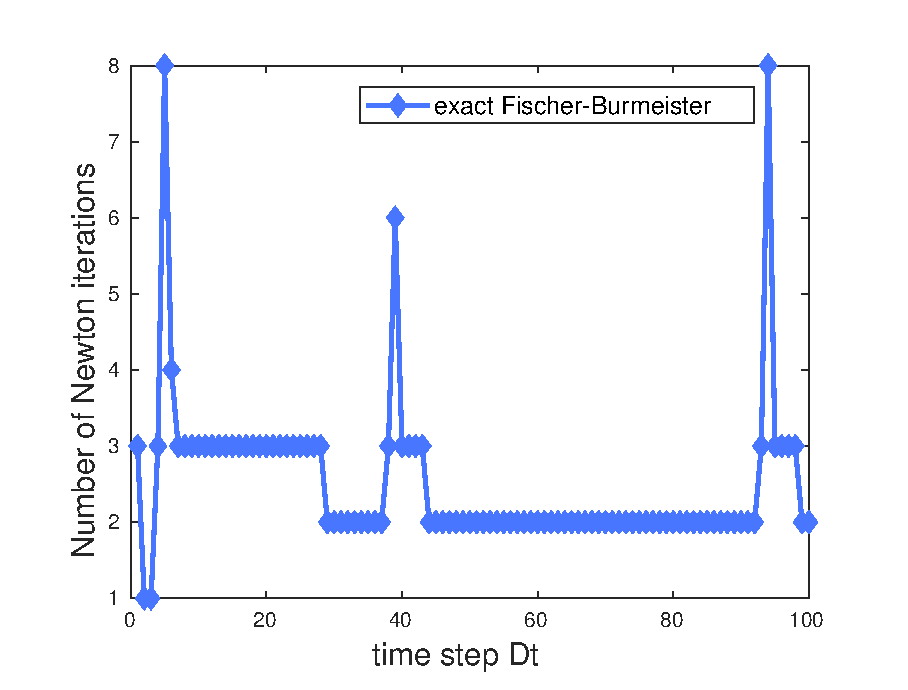
\includegraphics[scale=0.4]{number_newton_fischer_burmeister_per_time}
% \end{figure}
% \end{minipage}
% \begin{minipage}[c]{0.5 \linewidth}
% \begin{figure}[H]
% \includegraphics[scale=0.4]{number_newton_Mangasarian_per_time}
% \end{figure}
% \end{minipage}\hfill
% \begin{minipage}[c]{0.5 \linewidth}
% % \item\
% % The \textbf{Newton-min} algorithm requires less iterations.\\
% \begin{thebibliography}{10}
% \tiny{
% \bibitem{Facchinei:2003}
% {\sc F.~Facchinei and J.-S. Pang}, {\em Finite-dimensional variational
%   inequalities and complementarity problems. {V}ol. {I,II}}, Springer-Verlag, New York, 2003.
% }
% \end{thebibliography}
% \end{minipage}
% \end{frame}

% \begin{frame}
% \frametitle{Stopping criteria}

% \textcolor{cadmiumgreen}{\textbf{Stopping criteria for exact resolution:}}
% \begin{equation*}
% \mbox{\textcolor{blue}{\textbf{algebraic solver:}}} \left\|\bR^{n,\kk,\ii}\right\|_{\mathrm{rel}} \leq \epsalg
% \end{equation*} 
% \begin{equation*}
% \mbox{\textcolor{blue}{\textbf{semismooth Newton solver:}}} \: \left\|\ScKn(\bU^{n,\kk,\ii})\right\|_{\mathrm{rel}} \leq \epslin
% \vspace{0.5  cm}
% \end{equation*}
% \textcolor{cadmiumgreen}{\textbf{Stopping criteria for inexact resolution:}}
% \begin{equation*}
% \mbox{\textcolor{blue}{\textbf{algebraic solver:}}}
%  \left\|\bR^{n,\kk,\ii}\right\|_{\mathrm{rel}} \leq \alphaialg \left\|\ScKn(\bU^{n,\kk,\ii})\right\|_{\mathrm{rel}}  
% \end{equation*}
% \begin{equation*}
%   \quad \mbox{\textcolor{blue}{\textbf{semismooth Newton solver:}}} \: \left\|\ScKn(\bU^{n,\kk,\ii})\right\|_{\mathrm{rel}} \leq \epslin
% \vspace{0.5 cm}
% \end{equation*}

% \alert{\textbf{Question:}}
% Is it possible to save more iterations?
% \begin{thebibliography}{10}
% \scriptsize{
% \bibitem{Dabaghi:2017}
% {\sc J.~Dabaghi, V.~Martin, and M.~Vohral{\'{\i}}k}, {\em Adaptive inexact
%   semismooth Newton methods for the contact problem between two membranes}.
% \newblock submitted for publication, 2017.
% }
% \end{thebibliography}

% \end{frame}

\section{A posteriori analysis}
\subsection{}

\begin{frame}
\frametitle{Bibliography}
% \textcolor{red}{\textbf{A posteriori error estimate:}}
% $\dps |||\bu-\uhki||| \leq \left\{\dps \sum_{\substack{K \in\Th}} \eta_K(\uhki)^2\right\}^{1/2}$.\\

% \alert{\textbf{Effectivity index:}} $\mathrm{I_{eff}}=\left\{\dps \sum_{\substack{K \in\Th}} \eta_K(\uhki)^2\right\}^{1/2} {\large /} \; {\dps|||\bu-\uhki|||} \quad \alert{\searrow 1} $ 
%\subsection{Bibliography}
\vspace{-0.3 cm}
\begin{block}{
\scriptsize{
\textcolor{white}{\textbf{Global overview}}
}}
      \begin{thebibliography}{10}
\scriptsize{
\bibitem{Prager:Synge:1947}
{\sc W.~Prager and J.~L. Synge}, {\em Approximations in elasticity based on the
  concept of function space}, Quart. Appl. Math, 1947.
\bibitem{Ainsworth:2000}
{\sc M.~Ainsworth and J.~T. Oden}, {\em A posteriori error estimation in finite element analysis}, Pure and Applied Mathematics, New York, 2000.
% \bibitem{Repin:2008}
% {\sc S.~Repin}, {\em A posteriori estimates for partial differential
%   equations},
%   Walter de Gruyter GmbH \& Co. KG, Berlin, 2008.
\bibitem{Verfurth:2013}
{\sc R.~Verf\"urth}, {\em A posteriori error estimation techniques for finite
  element methods}, Oxford, 2013.}
\end{thebibliography}
\end{block}
   
   \vspace{-0.2 cm}
\begin{block}{
\scriptsize{
\textcolor{white}{\textbf{Equilibrated flux reconstructions}}
}}

     \begin{thebibliography}{10}
\scriptsize{ 
\bibitem{Destuynder:1999}
{\sc P.~Destuynder and B.~M\'etivet}, {\em Explicit error bounds in a
  conforming finite element method}, Math. Comp, 1999.

\bibitem{Braess:Schoberl:2008}
{\sc D.~Braess and J.~Sch\"oberl}, {\em Equilibrated residual error estimator
  for edge elements}, Math. Comp, 2008.

\bibitem{VorErn:2013}
{\sc A.~Ern and M.~Vohral{\'{\i}}k}, {\em Adaptive inexact {N}ewton methods
  with a posteriori stopping criteria for nonlinear diffusion {PDE}s}, SIAM J.
  Sci. Comput, 2013.
}
\end{thebibliography}
\end{block}
\vspace{-0.1 cm}
\begin{block}{
\scriptsize{
\textcolor{white}{\textbf{Multiphase compositional flows}}
}}
\hspace{-0.7 cm}

\scriptsize{
 \begin{thebibliography}{10}

% \bibitem{VorWhee:2013}
% {\sc M.~Vohral{\'{\i}}k and M.~F. Wheeler}, {\em A posteriori error estimates,
%   stopping criteria, and adaptivity for two-phase flows}, Comput. Geosci, 2013.

\bibitem{DiPietroFlauraudVorYoussef:2014}
{\sc D.~A. Di~Pietro, E.~Flauraud, M.~Vohral{\'{\i}}k, and S.~Yousef}, {\em A
  posteriori error estimates, stopping criteria, and adaptivity for multiphase
  compositional {D}arcy flows in porous media}, J. Comput. Phys, 2014.

\bibitem{CancesPopVor:2013}
{\sc C.~Canc\`es, I.~S. Pop, and M.~Vohral{\'{\i}}k}, {\em An a posteriori error
  estimate for vertex-centered finite volume discretizations of immiscible
  incompressible two-phase flow}, Math. Comp, 2014.
\end{thebibliography}
}
\end{block}

\end{frame}

\begin{frame}
\frametitle{Weak solution}
\vspace{-0.7 cm}
\begin{equation*}
%\label{eq:def:space:X:Y}
\begin{split}
&X \egaldef L^2((0,\tF);H^1(\Omega)), \quad Y \egaldef H^1((0,\tF);L^2(\Omega)), \quad \widehat{Y} \egaldef H^1((0,\tF);L^{\infty}(\Omega)),\\
&  Z \egaldef \left\{v \in L^2((0,\tF);L^{\infty}(\Omega)), \hspace{0.15 cm} v \geq 0 \hspace{0.15 cm} \mbox{on} \hspace{0.15 cm} \Omega \times (0,\tF)  \right\}.
\end{split}
\end{equation*}
\pause
\vspace{-0.3 cm}
\begin{assumption}[Weak formulation]
\label{ref:assumption:weak:solution}
\vspace{-0.8 cm}\begin{align*}
&\Sl \in \widehat{Y}, \quad 1-\Sl \in Z, \quad \lw \in Y, \quad \lh \in Y, \quad \Pl \in X, \quad \chihl \in X,\\
&\left(\Phiw \egaldef \rhowl \darcyliq - \Jhl, \Phih \egaldef \rhohl \darcyliq + \rhohg \darcygas + \Jhl\right) \in \left[L^2((0,\tF); \HdivOmeg)\right]^2 ,\\
&\dps \int_{0}^{\tF} \left(\partial_t \lc, \varphi \right)_{\Omega}(t)\,\mathrm{dt}-\hspace{-0.1 cm}\int_{0}^{\tF} \left(\Phic, \nab \varphi \right)_{\Omega}(t)\,\mathrm{dt} = \hspace{-0.1 cm} \int_{0}^{\tF} \left(\Qc, \varphi \right)_{\Omega}(t)\,\mathrm{dt} \ \forall \varphi \in X, \  \forall \componentc \in \hspace{-0.05 cm}\left\{\componentw,\componenth\right\}\\
&\dps \int_{0}^{\tF} \left(\lambda - \left(1 - \Sl\right), H[\Pl+\Pcp(\Sl)]-\betal \chihl  \right)_{\Omega}(t)\,\mathrm{dt} \geq 0 \quad \forall \lambda \in Z, \\
&\nonumber\mbox{the initial condition  holds}.
\end{align*}
\end{assumption}
\pause
%We equip the space $X$ with the norm 
$\left\| \varphi \right\|_X^2 \egaldef \sum_{n=1}^{\Nt}\left\| \varphi \right\|_{X_n}^2\,\mathrm{dt}, \quad \left\| \varphi \right\|_{X_n} \egaldef  \int_{\In} \sum_{K \in \Th} \left\| \varphi \right\|_{X,K}^2 \, \mathrm{dt},$

Define space-time functions:\begin{equation}
\label{eq:def:functions:space:time}
\begin{split}
&\Plhtaunki(t^n) = \Phnki \in \textcolor{cadmiumgreen}{\PtwodTh}, \hspace{0.06 cm} \tildePhtaunki(t^n) = \tildePhnki \in \textcolor{cadmiumgreen}{\PtwocTh}, \hspace{0.06 cm} \lchtaunki(t^n) = \lchnki\in \textcolor{cadmiumgreen}{\PzerodTh}, \\ 
&\Shtaunki(t^n) = \Shnki \in \textcolor{cadmiumgreen}{\PzerodTh}, \hspace{0.06 cm}
 \chihtaunki(t^n) = \chihnki \in \textcolor{cadmiumgreen}{\PtwodTh}, \hspace{0.06 cm} \tildechihtaunki(t^n) = \tildechihnki \in \textcolor{cadmiumgreen}{\PtwocTh}.
\end{split}
\end{equation}
\end{frame}
\begin{frame}
\frametitle{Error measure}
\vspace{-0.2  cm}
\textcolor{cadmiumgreen}{\textbf{Dual norm of the residual for the components}}
\vspace{-0.15 cm}
\begin{equation*}
\hspace{-0.2 cm}\left\|\mathcal{R}_{\componentc}(\Shtau,\Phtau,\chihtau) \right\|_{\Xn'} = \sup_{\varphi \in \Xn, \left\|\varphi\right\|_{\Xn} = 1}  \int_{\In} 
\left(\Qc - \partial_t \lchtau , \varphi\right)_{\Omega}(t) + \left(\Phichtau,\nab \varphi \right)_{\Omega}(t)\,\mathrm{dt} .
%\label{eq:dual:norm:residual}
\vspace{-0.25 cm}
\end{equation*}
\textcolor{cadmiumgreen}{\textbf{Residual for the constraints}}
\begin{equation*}
  \mathcal{R}_{\mathrm{e}}(\Shtau,\Phtau,\chihtau) = \int_{\In}\left(\textcolor{electricpurple}{1 - \Shtau}, \textcolor{carmine}{H \left[\Phtau + \Pcp(\Shtau)\right] - \betal \chihtau} \right)_{\Omega}(t)\,\mathrm{dt}.
\end{equation*}
\vspace{-0.3 cm} 
\textcolor{cadmiumgreen}{\textbf{Error measure for the nonconformity of the pressure}}
\begin{equation*}
%\label{eq:error:measure:nonc:presure}
\mathcal{N}_{P}(\Phtau) \egaldef \inf_{\delta_{\phasel} \in \Xn} \left\{\sum_{\componentc \in \left\{ \componentw,\componenth \right\}} \int_{\In} 
  \left\| \tensor \frac{\krl(\Shtau)}{\mul} \rhocl \nab \left(\Phtau-\delta_{\phasel}  \right)(t) \right\|^2 \,\mathrm{dt} \right\}^{\frac{1}{2}},
\end{equation*}

\vspace{-0.15 cm}
\textcolor{cadmiumgreen}{\textbf{Error measure for nonconformity of the molar fraction}}
\vspace{-0.3 cm}
\begin{equation*}
%\label{error:measure:nonc:molar:frac}
\mathcal{N}_{\chi}(\chihtau) \egaldef\inf_{\theta \in \Xn} \left\{\int_{\In} \left\| -\porosity \Mh \Shtau \left(\frac{\rhowl}{\Mw} + \frac{\betal}{\Mh}\chihtau \right) \Dhl \nab \left(\chihtau-\theta \right)(t) \right\|^2 \,\mathrm{dt} \right\}^\frac{1}{2},
\end{equation*}
\vspace*{-0.3 cm}
\begin{definition}[Error measure]
\vspace{-0.5 cm}
\begin{equation*}
\mathcal{N}^n = \left\{\sum_{\componentc \in\mathcal{C}} \left\|\mathcal{R}_{\componentc}(\Shtau,\Phtau,\chihtau) \right\|_{X_n'}^2 \right\}^{\frac{1}{2}} + \left\{\sum_{\phasep \in \mathcal{P}}\mathcal{N}_{\phasep}^2 + \mathcal{N}_{\chi}^2\right\}^{\frac{1}{2}} + \mathcal{R}_{\mathrm{e}}(\Shtau,\Phtau,\chihtau)
\label{eq:norm:aposteriori}
\end{equation*}
\end{definition}
\end{frame}
\begin{frame}
\frametitle{Finite volume linearization}
\textcolor{cadmiumgreen}{\textbf{The finite volume scheme provides}}
\begin{equation*} 
  |K| \partial_t^n \lcK + \sum_{\sigma \in \EK} {F}_{\componentc,K,\sigma}(\bUn) =  |K|\QcKn,
\end{equation*}
\textcolor{cadmiumgreen}{\textbf{Inexact semismooth linearization}}

\begin{equation*}
\label{eq:flux:equation}
 \frac{|K|}{\Delta t}\left[\lcK\left(\bU^{n,\kk-1}\right) - \lcK^{n-1} + \mathcal{L}_{\componentc,K}^{n,\kk,\ii}\right] + \sum_{\sigma \in \EKint} \mathcal{F}_{\componentc,K,\sigma}^{n,\kk,\ii}- |K|\QcKn + {\bR}_{\componentc,K}^{n,\kk,\ii} = 0
\end{equation*}
 \textcolor{blue}{Linear perturbation in the accumulation}
\begin{equation*}
\mathcal{L}_{\componentc,K}^{n,\kk,\ii} = \sum_{K' \in \Th} \frac{|K|}{\Delta t}  \frac{\partial \lcK^n}{\partial \bU_{K'}^n}(\bU_{K'}^{n,\kk-1}) \left[\bU_{K'}^{n,\kk,\ii}-\bU_{K'}^{n,\kk-1} \right],
\end{equation*}
\textcolor{blue}{Linearized component flux}
\begin{equation*}
\label{eq:linearized:semi:smooth:component:flux}
\mathcal{F}_{\componentc,K,\sigma}^{n,\kk,\ii} = \sum_{K' \in \Th} \frac{\partial {F}_{\componentc,K,\sigma}}{\partial \bU_{K'}^n} \left(\bU^{n,\kk-1}\right) \left[\bU_{K'}^{n,\kk,\ii} -\bU_{K'}^{n,\kk-1} \right] + {F}_{\componentc,K,\sigma}\left(\bU^{n,\kk-1}\right).
\end{equation*}
\end{frame}

\begin{frame}
\frametitle{Raviart Thomas spaces}
\vspace{-0.3 cm}
\begin{definition}
The lowest-order Raviart--Thomas space is defined by
\begin{equation*}
\textbf{RT}_0(\Omega)=\left\{\bw_h \in \HdivOmeg, {\bw_h}|_{K} \in \textbf{RT}_0(K)\ \forall K \in \Th\right\}
\end{equation*}
 \begin{equation*}
 \quad \textbf{RT}_0(K)=[{\mathbb{P}}_0(K)]^2 + \vec{{\bm x}} \cdot  {\mathbb{P}}_0(K)
\end{equation*}
\end{definition}
\vspace{0.3 cm}
\begin{minipage}[c]{0.5 \linewidth}
\begin{figure}
\centering
\begin{tikzpicture}
%\draw [very thin, gray] (0,0) grid (8,5);
\draw(1,2)--(5,2)--(3,5)--(1,2);
\draw [thick, blue] [->] (3,2) -- (3,1);
\draw [thick, blue] [->] (4,3.5) -- (5,4.2);
\draw [thick, blue] [->] (2,3.5) -- (1,4);
\draw [fill] (4,3.5) circle (0.09); %node {$\bullet$};
\draw [fill] (2,3.5) circle (0.09); %node {$\bullet$};
\draw [fill] (3,2) circle (0.09); %node {$\bullet$};
\end{tikzpicture}
\end{figure}
\end{minipage}\hfill
\begin{minipage}[c]{0.5 \linewidth}
\textcolor{cadmiumgreen}{\textbf{Degrees of freedom $\textbf{RT}_0$:}} 
\begin{equation*}
v_j=(\bv \cdot \bn_{e_j},1)_{e_j}, \hspace{0.2 cm} e_j \in \partial K, \hspace{0.2 cm} j = \left\{1,2,3\right\}.
\end{equation*}
% \begin{proposition} 
% If $\bv \in \textbf{RT}_0(\Omega)$ then $v|_{K} \cdot \bn_{K,\sigma}$ is constant over the edge $\sigma$.
% \end{proposition}
\end{minipage}

\end{frame}
\begin{frame}
\frametitle{Phase pressure reconstruction}
\centering
\includegraphics[width = 0.7 \textwidth]{image_oswald}
 
\begin{figure}
\includegraphics[scale=0.55]{image/modif_image_post_process_cont}   
\end{figure}
\end{frame}
% \begin{frame}
% \frametitle{Phase pressure reconstruction}

% \textcolor{cadmiumgreen}{\textbf{ $P_K^{n,\kk, \ii}$ constant $\Rightarrow \nab P_K^{n,\kk, \ii} =0$.}} Define $\left({\bm \xi}_{\phasel,h}^{n,\kk, \ii},{\bm \xi}_{\phaseg,h}^{n,\kk, \ii}\right) \in \RTO(K) \times \RTO(K)$
%  \begin{equation*}
%  \left({\bm \xi}_{\phasel,h}^{n,\kk, \ii}\cdot \bn_K,1\right)_{\sigma} = -|\sigma| \frac{\PLnki - \PKnki}{d_{KL}} \forall K \in \Th \ \forall \sigma \in \EKint, 
% \end{equation*}
% \begin{equation*} 
% \hspace{-0.3 cm}\left({\bm \xi}_{\phaseg,h}^{n,\kk, \ii}\cdot \bn_K,1\right)_{\sigma} = - \frac{|\sigma| }{d_{KL}} \left[\PLnki+\Pcp(\SLnki) - \PKnki - \Pcp(\SKnki) \right] \forall K \in \Th \ \forall \sigma \in \EKint
%  \end{equation*}
% The \textbf{quadratic discontinuous} liquid phase pressure $\Phnki$ and gas phase pressure $\Phathnki$ satisfy
% \vspace{-0.2 cm}
% \begin{equation*}
% \hspace{-0.2 cm}
% \left(- \nab \Phnki \right)|_{K} = \left({\bm \xi}_{\phasel,h}^n \right)_K  \hspace{0.15 cm} \mbox{and} \hspace{0.15 cm} \left(\Phnki,1 \right)_K = |K|\PKnki
% \end{equation*}
% \begin{equation*}
% \hspace{-0.2 cm}
% \left(-\nab \Phathnki \right)|_{K} = \left({\bm \xi}_{\phaseg,h}^{n,\kk, \ii} \right)_K \hspace{0.15 cm} \mbox{and} \hspace{0.15 cm} \left(\Phathnki,1 \right)_K = |K| \left(\PKnki + \Pcp(\SKnki) \right)
% \end{equation*}
%  \textcolor{red}{\textbf{The Oswald interpolation operator}}
% defines continous $\mathbb{P}_2$ functions:
% \begin{itemize}
% \item $I_{\mathrm{os}}(\Phnki) \in \mathbb{P}_2 \cap H_0^1(\Omega)$\\
% \item  $I_{\mathrm{os}}(\Phathnki) \in \mathbb{P}_2 \cap H_0^1(\Omega)$ 
% \end{itemize}
% \end{frame}

% \begin{frame}
% \frametitle{Mole fraction reconstruction}
% \textcolor{cadmiumgreen}{\textbf{Phase pressure $\chiKnki$ is constant $\Rightarrow \nab \chiKnki=0$.}}
% Define ${\bm \nu}_{\phasel,h}^{n,\kk, \ii} \in \RTO(K) $
% \begin{equation*}
%  \left({\bm \nu}_{\phasel,h}^n\cdot \bn_K,1\right)_{\sigma} := -|\sigma| \frac{\chiLnki-\chiKnki}{d_{KL}} \quad \forall K \in \Th \quad \forall \sigma \in \EKint.
% \end{equation*}
% The \textbf{quadratic discontinuous} mole fraction pressure $\chihnki$ satisfies
% \begin{equation*}
% \left(-\nab \chihnki \right)|_{K} := \left({\bm \nu}_{\phasel,h}^{n,\kk,\ii} \right)_K \quad \mbox{and} \quad \frac{\left(\chihnki,1 \right)_K}{|K|} := \chiKnki
% \end{equation*}
% \textcolor{red}{\textbf{The Oswald interpolation operator}}
% defines continous $\mathbb{P}_2$ function:
% \begin{itemize}
% \item $I_{\mathrm{os}}(\chihnki) \in \mathbb{P}_2 \cap H_0^1(\Omega)$
% \end{itemize}
% \end{frame}



\begin{frame}
\frametitle{Component flux reconstructions}
\textcolor{cadmiumgreen}{\textbf{Discretization error flux reconstruction:}}
\begin{equation*}
\left(\Thetachdiscnki \cdot \bn_K,1 \right)_{\sigma} = F_{\componentc,K,\sigma}\left(\bU^{n,\kk, \ii}\right) \quad \forall K \in \Th
\end{equation*}
\vspace{-0.1 cm}
\textcolor{cadmiumgreen}{\textbf{Linearization error flux reconstruction:}}
\begin{equation*}
\left(\Thetachlinnki \cdot \bn_K,1 \right)_{\sigma} = \mathcal{F}_{\componentc,K,\sigma}^{n,\kk,\ii} -  F_{\componentc,K,\sigma}\left(\bU^{n,\kk, \ii}\right) \quad \forall K \in \Th,
\end{equation*}
\vspace{-0.1 cm}
\textcolor{cadmiumgreen}{\textbf{Algebraic error flux reconstruction:}}
\begin{equation*}
\Thetachalgnkinu  \egaldef {\bm \Theta}_{\componentc,h,\mathrm{disc}}^{n,\kk,\ii+\nuu} + {\bm \Theta}_{\componentc,h,\mathrm{lin}}^{n,\kk,\ii+\nuu} - \left(\Thetachdiscnki + \Thetachlinnki \right)
 \quad \forall K \in \Th
\end{equation*}
\textcolor{red}{\textbf{Total flux reconstruction:}} 
\begin{equation*}
%\label{eq:def:tot:flux}
\Thetachnkinu = \Thetachdiscnki+\Thetachlinnki+\Thetachalgnkinu
\end{equation*}
\vspace{-0.2 cm}
\begin{proposition}[Equilibration property]
\begin{equation*}
\left(\QcKn - \frac{\lcK(\bU^{n,\kk-1})-\lcK^{n-1} + \LcK^{n,\kk, \textcolor{burntorange}{i + \nu}}}{\tau_n} - \nab \cdot \Thetachnkinu,1\right)_K=R_{\componentc,K}^{n,\kk,\ii+ \nuu}
\end{equation*}
\end{proposition}
\end{frame}
%
\begin{frame}
\frametitle{Error estimators}
\begin{remark}
$\partial_t \lc + \nab \cdot \Thetachnkinu \neq \Qc$ and $\Thetachnkinu \neq \Phichtaunki(t^n)$ and $1 - \Shtaunki \ngeq 0$ and $H\left[\Phtaunki \hspace{-0.1 cm}+\hspace{-0.1 cm} \Pcp\left(\Shtaunki\right)\right]\hspace{-0.1 cm}-\betal \chihtaunki \ngeq 0$ and $\Phtaunki \notin X$ and $\chihtaunki \notin X$
\end{remark}
\textcolor{cadmiumgreen}{\textbf{Discretization estimator}}
\begin{equation*}
\begin{split}
&\etaRKcnkinu = \min\left\{\CPW,\varepsilon^{-\frac{1}{2}}\right\} h_K \left\|\Qchn - \frac{\lcK(\bU^{n,\kk-1}) - \lcK^{n-1} + \mathcal{L}_{\componentc,K}^{n,\kk,\ii}}{\Tn} - \nab \cdot \Thetachnki \right\|_K \\
&\etaFKcnkinu(t) = \left\|\Thetachnkinu - \Phichtaunki(t) \right\|_K\\
&\etaPKposnki(t) =\left(\left\{1-\Shtaunki\right\}^{+}(t),\left\{H\left[\Phtaunki + \Pcp\left(\Shtaunki\right)\right]-\betal \chihtaunki\right\}^{+}(t)\right)_K\\
&\etaNCKlcnki(t) = \left\| \tensor \frac{\krl(\Shtaunki)}{\mul} \rhocl \nab \left(\Phtaunki-\tildePhtaunki  \right)(t) \right\|_K\\
&\etaNCKchinki(t)  = \left\| -\porosity \Mh \Shtaunki \left(\frac{\rhowl}{\Mw} + \frac{\betal}{\Mh}\chihtaunki \right) \Dhl \nab \left(\chihtaunki-\tildechihtaunki \right)(t) \right\|_K
\end{split}
\end{equation*}
\end{frame}
%
\begin{frame}
\frametitle{Error estimators}
\textcolor{cadmiumgreen}{\textbf{Linearization estimator}}
\begin{equation*}
\begin{split}
& \etaNAKcnki  = \varepsilon^{-\frac{1}{2}} h_K \left(\Tn\right)^{-1} \left\|\lcK(\bU^{n,\kk,\ii}) - \lcK(\bU^{n,\kk-1}) - \mathcal{L}_{\componentc,K}^{n,\kk,\ii} \right\|_K\\
& \etaPKnegnki(t)  = \left(\left\{1 - \Shtaunki\right\}^{-}(t),\left\{H\left[\Phtaunki + \Pcp\left(\Shtaunki\right)\right]-\betal \chihtaunki\right\}^{-}(t)\right)_K
\end{split}
\end{equation*}
\textcolor{cadmiumgreen}{\textbf{Algebraic estimator}}
\begin{equation*}
\begin{split}
\etaalgKcnki & \egaldef \left\|\Thetachalgnkinu \right\|_K\\
\etaremcKnkinu & \egaldef h_K |K|^{-1} \varepsilon^{-\frac{1}{2}} \left\|\RcK^{n,\kk,\ii+\nuu}  \right\|_K
\end{split}
\end{equation*}

\begin{theorem}
\begin{equation*}
%\label{eq:corrolary:component:error}
\mathcal{N}^{n,\kk,\ii} \leq \etadiscnki + \etalinnki + \etaalgnki
\end{equation*}  
\end{theorem}
\end{frame}

 \begin{frame}
 \frametitle{Adaptivity}
 \vspace{-0.3 cm}\begin{algorithm}[H]
 \caption{Adaptive inexact semismooth Newton algorithm}
 \begin{algorithmic}

 \STATE{\textbf{Initialization:}\; Choose an initial vector $\bU^{n,\textcolor{royalblue}{0}} \in \R^{3 \Nh}$, ($\kk=0$)}\\
 \STATE{\textbf{Do}}\\
 \STATE{\quad$\kk = \kk+1$}\\
 \STATE {\quad Compute $\mathbb{A}^{n,\kk-1}  \in \R^{3 \Nh, 3 \Nh}$, \quad $\bB^{n,\kk-1} \in \R ^{3 \Nh}$ \\
 \quad Consider  the system of linear algebraic equations 
 $\mathbb{A}^{n,\textcolor{royalblue}{k-1}} \bU^{n,\kk}= \bB^{n,\textcolor{royalblue}{k-1}}$}
 \STATE{\quad \textbf{Initialization for the linear solver:} Define $\bU^{n,\kk,\textcolor{burntorange}{0}} = \bU^{n,\kk-1}$, ($\textcolor{burntorange}{i=0}$) 
 as}
 \STATE{\quad initial guess for the linear solver}\\
 \STATE{\quad \textbf{Do}}
 	\STATE{\qquad $\textcolor{burntorange}{i=i+1}$}\\	
 	\STATE \qquad Compute Residual: {$\bR^{n,\kk, \ii} =\bB^{n,\textcolor{royalblue}{k-1}}-\mathbb{A}^{n,\textcolor{royalblue}{k-1}} \bU^{n,\kk, \ii}$}\\
 	\qquad  Compute estimators 
 	\STATE{\quad \textbf{While} \fcolorbox{violet}{white}{$\eta_{\mathrm{alg}}^{n,\kk,\ii} \geq \gamma_{\mathrm{alg}} \max  \left\{{\eta_{\mathrm{disc}}^{n,\kk,\ii}, \eta_{\mathrm{lin}}^{n,\kk,\ii}}\right\}$}} 
		
 	\STATE{\textbf{While} \fcolorbox{violet}{white}{ $\eta_{\mathrm{lin}}^{n,\kk,\ii} \geq \gamma_{\mathrm{lin}} \eta_{\mathrm{disc}}^{n,\kk,\ii}$}} 
 	\STATE{\textbf{End}}
 \end{algorithmic}
 \end{algorithm}
 
 \end{frame}
%
\section{Numerical experiments}
\subsection{}
\begin{frame}
\frametitle{Numerical experiments}
%
$\Omega$:  one-dimensional core with length $L = 200 m$. We consider the \textbf{semismooth Newton-min solver} in combination with the \textbf{GMRES} algebraic solver.\\
$\Delta t = 5000$ years, $\Nsp = 1000$ cells, $\tF = 5 \times 10^{5}$ years.
\begin{figure}
\includegraphics[width= 1 \textwidth]{image/num_exp_finite_vol}
\end{figure}
% \begin{minipage}{.25 \linewidth}
% \textcolor{blue}{Gas injection}\hspace{0.1 cm}$\blacktriangleright$ \hspace{-0.3 cm} $\blacktriangleright$ 
% \end{minipage}
% \hfill
% \begin{minipage}{.55 \linewidth}
%  \begin{figure}[htbp]
% \vspace{-1 cm}
%  \centering 
% \hspace{-5.5 cm}\begin{picture}(180,60)(0,0)
%  \thicklines
% \put(0,15){\line(180,0){180}}
% %\put(0,10){\red{\line(0,10){10}}}
% %\put(0,0){\makebox(0,0){\small \red{$t_0$}}}
% \put(0,15){\black{\circle*{6}}}
% \put(15,15){\red{\circle*{6}}}
% %\put(30,15){\red{\circle*{6}}}
% \put(45,15){\red{\circle*{6}}}
% %\put(60,15){\red{\circle*{6}}}
% \put(75,15){\red{\circle*{6}}}
% %\put(90,15){\red{\circle*{6}}}
% \put(105,15){\red{\circle*{6}}}
% %\put(120,15){\red{\circle*{6}}}
% \put(135,15){\red{\circle*{6}}}
% %\put(150,15){\red{\circle*{6}}}
% \put(165,15){\red{\circle*{6}}}
% \put(180,15){\black{\circle*{6}}}
% \end{picture}
% %\caption{Time discretization of the model}
% %\label{ref:time:discretization:model}
% \mbox{\textcolor{blue}{liquid}}
% \end{figure}
% \end{minipage}\\
\textcolor{cadmiumgreen}{\textbf{Van Genuchten--Mualem model:}}
\begin{equation*}
\Pcp(\Sl)=P_r\left(S_{\mathrm{le}}^{-\frac{1}{m}}-1\right)^{\frac{1}{n^{*}}}
\end{equation*}
\begin{equation*}
\krl(\Sl)=\sqrt{S_{\mathrm{le}}} \left(1 - (1-S_{\mathrm{le}}^{\frac{1}{m}})^m  \right)^2, \; \krg(\Sl)=\sqrt{1 - S_{\mathrm{le}}} \left(1 - S_{\mathrm{le}}^{\frac{1}{m}} \right)^{2m}
\end{equation*}    
with 
\begin{equation*}
S_{\mathrm{le}}=\frac{\Sl-S_{\mathrm{lr}}}{1-S_{\mathrm{lr}}-S_{\mathrm{gr}}} \quad \mbox{and} \quad m=1-\frac{1}{n^{*}}
\end{equation*}
\end{frame}
\begin{frame}
\frametitle{Numerical experiments}
\textcolor{blue}{\textbf{Solution at $t = 1.05 \times 10^{5}$ years}}
\begin{figure}
\centering
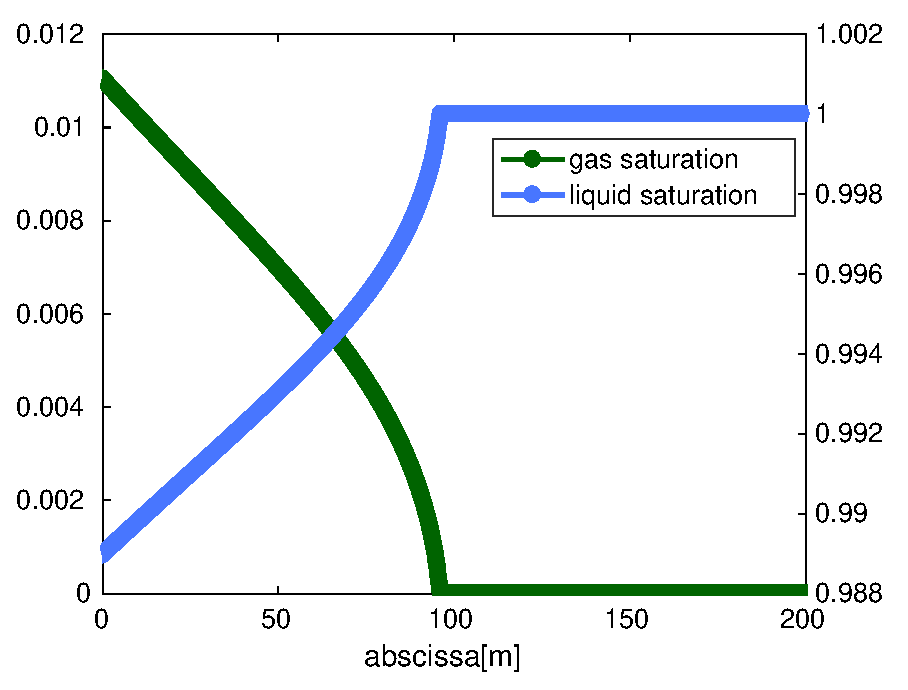
\includegraphics[width=0.33\textwidth]{image/saturations_cv_solver_1000_cells_nt=20}
\includegraphics[width=0.33\textwidth]{image/liquid_pressure_cv_solver_1000_cells_nt=20}
\includegraphics[width=0.33\textwidth]{image/mole_frac_cv_solver_1000_cells_nt=20}
\end{figure}
\textcolor{blue}{\textbf{Complementarity constraints at}} $\kk = 4$ \textcolor{blue}{\textbf{and}} $\ii = 2$
\begin{figure}
\centering
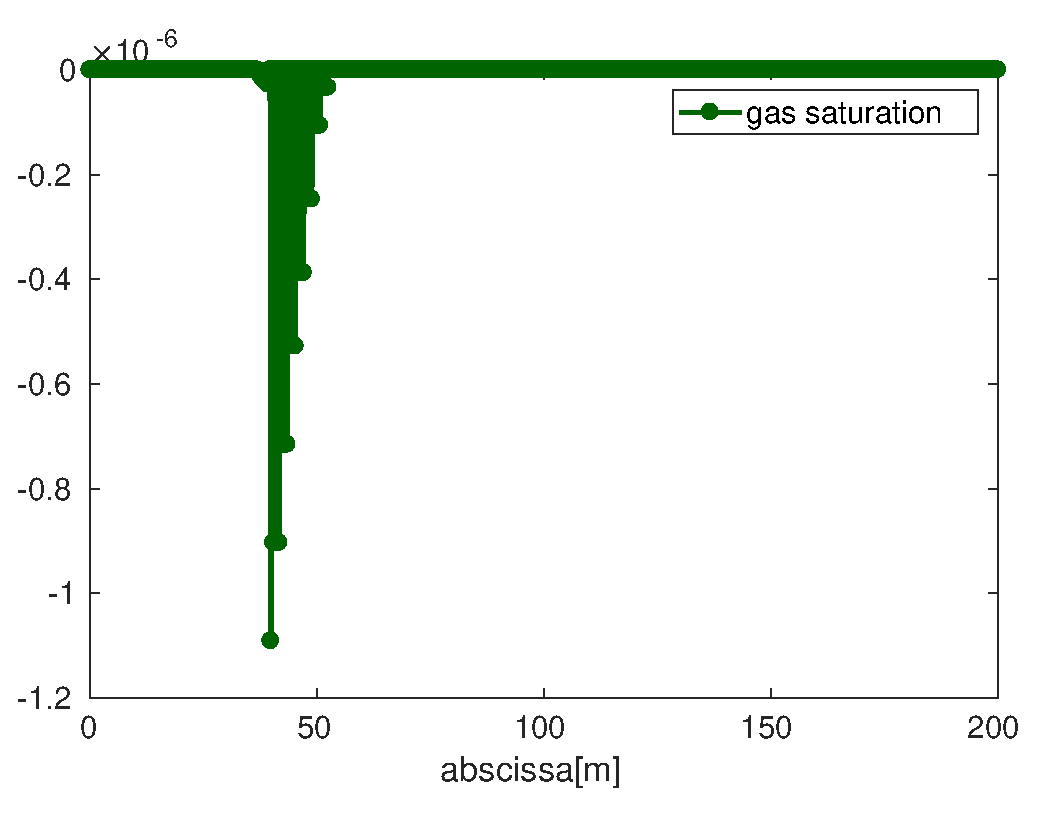
\includegraphics[width=0.355\textwidth]{image/gas_saturation_neg_gmres_iter2_newtoninter_4} \qquad
\includegraphics[width=0.37\textwidth]{image/henry_constraint_neg_gmresiter2_newton_iter4}
\end{figure}
\end{frame}
%
\begin{frame}
\frametitle{Phase transition estimator}
\begin{minipage}{0.49\textwidth}
\centering
\scriptsize{\textcolor{red}{\textbf{\bm{$t=2500$} years}}}
\includegraphics[width=0.78\textwidth]{image/MODIF_phase_transition_estimator_appearance_gas_nt=inittime_cv}
\end{minipage}
%\hfill
\hfill
\begin{minipage}{0.49\textwidth}
\centering
\scriptsize{\textcolor{red}{ \textbf{\bm{$t = 1.25 \times 10^4$} years}}} 
\includegraphics[width=0.78\textwidth]{image/MODIF_phase_transition_estimator_appearance_gas_nt=2_cv}
\end{minipage}

% % \vspace{-0.3 cm}
 \begin{minipage}{.49 \textwidth}
 \hspace{2 cm}\scriptsize{ \textbf{\textcolor{red}{ \bm{$t = 4.25 \times 10^4$} years}}}
\vspace{-0.3 cm}
\begin{figure}
\includegraphics[width=0.79\textwidth]{image/MODIF_phase_transition_estimator_appearance_gas_nt=9_cv}
\end{figure}
 \end{minipage}
\begin{minipage}{.49 \textwidth}
\begin{remark}
This estimator detects the error caused by the 
 appearance of the gas phase whenever the gas spreads throughout the domain. 
\end{remark}
\end{minipage}
\end{frame}
\begin{frame}
\frametitle{Newton-min adaptivity}
\vspace{-0.1 cm}
\hspace{2 cm} \scriptsize{\textcolor{red}{\textbf{Exact Newton-min}}} \hspace{4.5 cm} \scriptsize{\textcolor{red}{\textbf{Inexact Newton-min}}}
\vspace{-0.1 cm}
\begin{figure}
\includegraphics[scale=0.35]{image/estimators_exact_resolution_newton_iter_nt=21_tolnewton_10-6_tolgmres_10-11}
\qquad \qquad \qquad \includegraphics[scale=0.32]{image/estimators_inex_resolution_newton_iter_nt=21_stopp_crit_alg_modif}
\end{figure}
\hspace{4.8 cm}\scriptsize{\textcolor{red}{\textbf{Adaptive inexact Newton-min}}}
\vspace{-0.15 cm}\begin{figure}
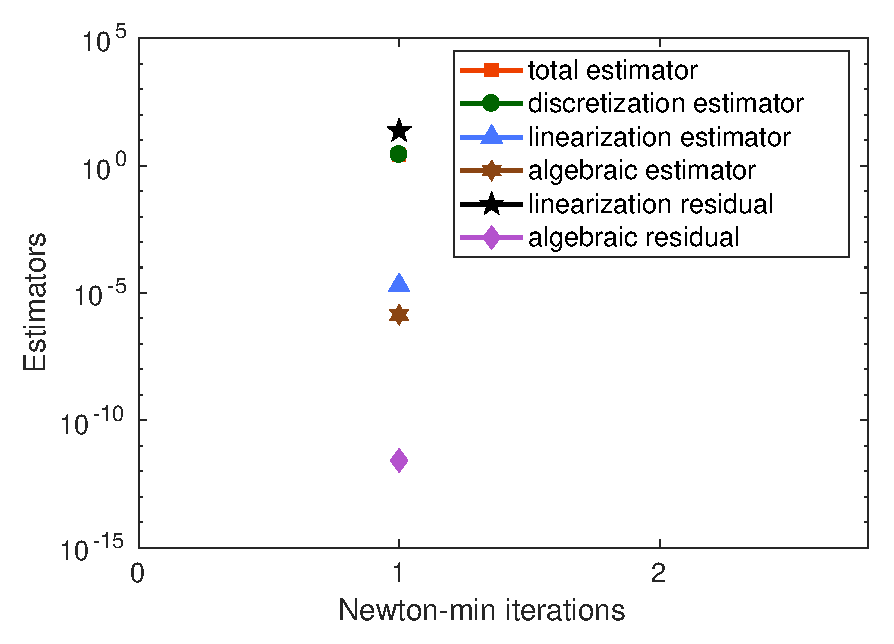
\includegraphics[scale=0.35]{image/estimators_adapt_inexact_resolution_newton_iter_nt=20}
\end{figure}
\end{frame}
%
\begin{frame}
\frametitle{GMRES adaptivity}
\hspace{2 cm}\scriptsize{\textcolor{red}{\textbf{Exact Newton-min}}} \hspace{4.8 cm}\scriptsize{\textcolor{red}{\textbf{Inexact Newton-min}}}
\vspace{-0.1 cm}
\begin{figure}
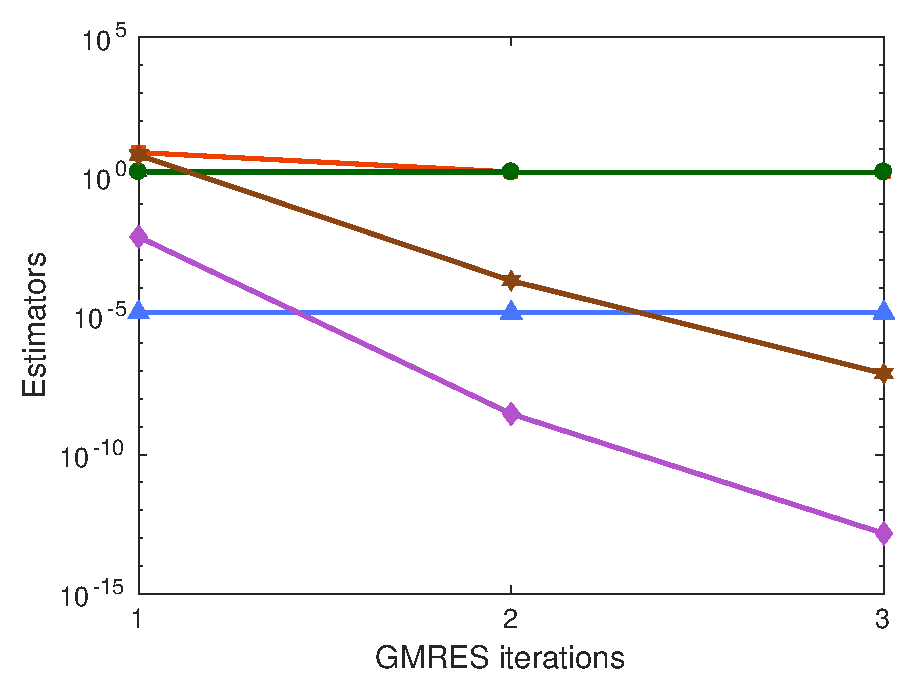
\includegraphics[width=0.41\textwidth]{image/estimators_exact_resolution_gmres_iter_newton_iter1_tol_newton_10-6_tol_gmres_10-12nt=21} \qquad \qquad \qquad \qquad
\includegraphics[width=0.41\textwidth]{image/estimators_inex_resolution_newton_iter_1gmres_iter_nt=21}
\end{figure}
\vspace{-0.2 cm}
\hspace{5 cm}\scriptsize{\textcolor{red}{\textbf{Adaptive inexact Newton-min}}}
\vspace{-0.2 cm}
\begin{figure}
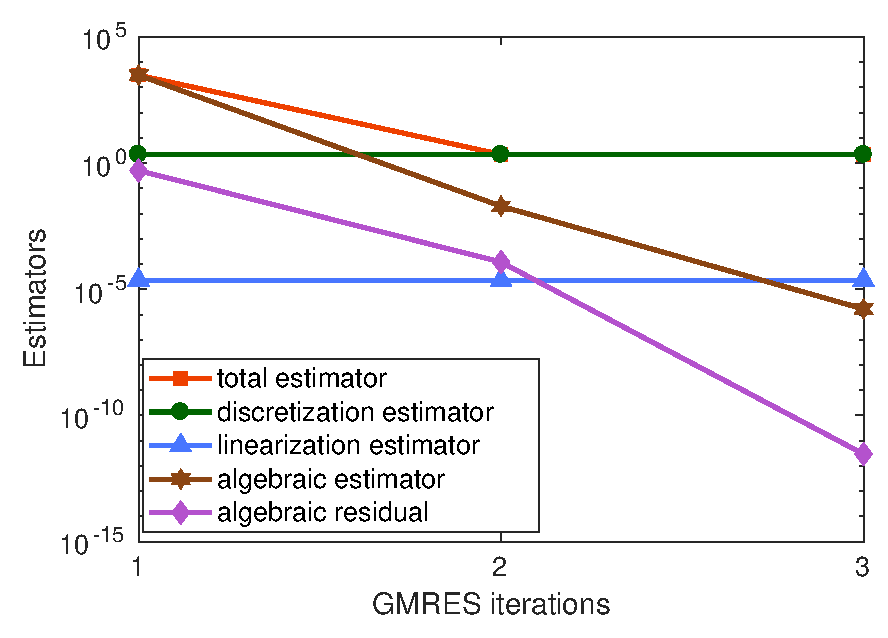
\includegraphics[width=0.41\textwidth]{image/estimators_adapt_inex_resolution_newton_iter_1gmres_iter_nt=21}
\end{figure}
\end{frame}
\begin{frame}
\frametitle{Overall performance}
\vspace{-0.2 cm}
\begin{figure}
\centering
\includegraphics[width=0.44\textwidth]{image/number_Newton_iterations_three_methods_per_time_Nx_1000}
\hspace{1 cm}
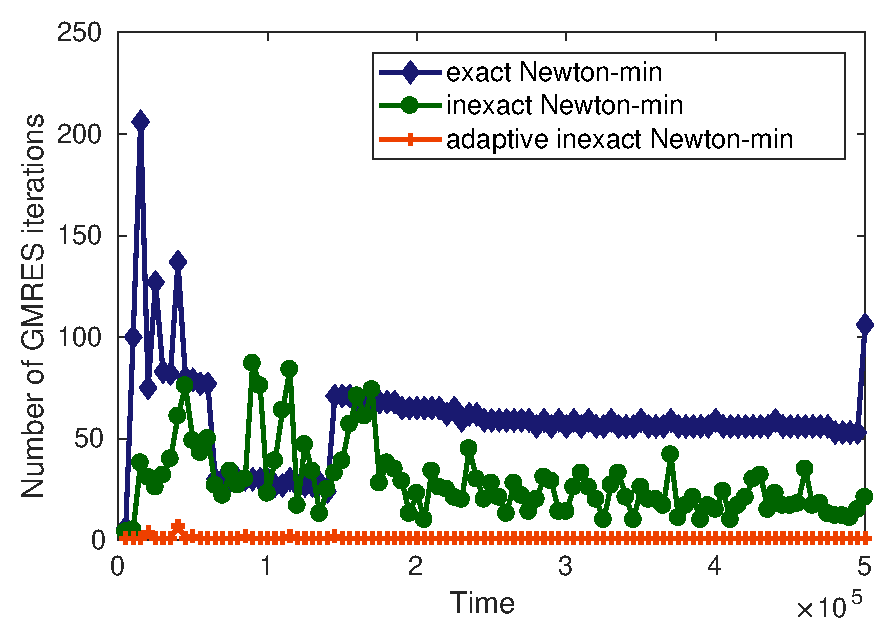
\includegraphics[width=0.44\textwidth]{image/number_gmres_iterations_three_methods_per_time_Nx_1000}
\end{figure}
\vspace{-0.3 cm}
\begin{figure}
\centering
\includegraphics[width=0.44\textwidth]{image/Cumulated_number_Newton_iterations_three_methods_Nx_1000}
\hspace{1 cm}
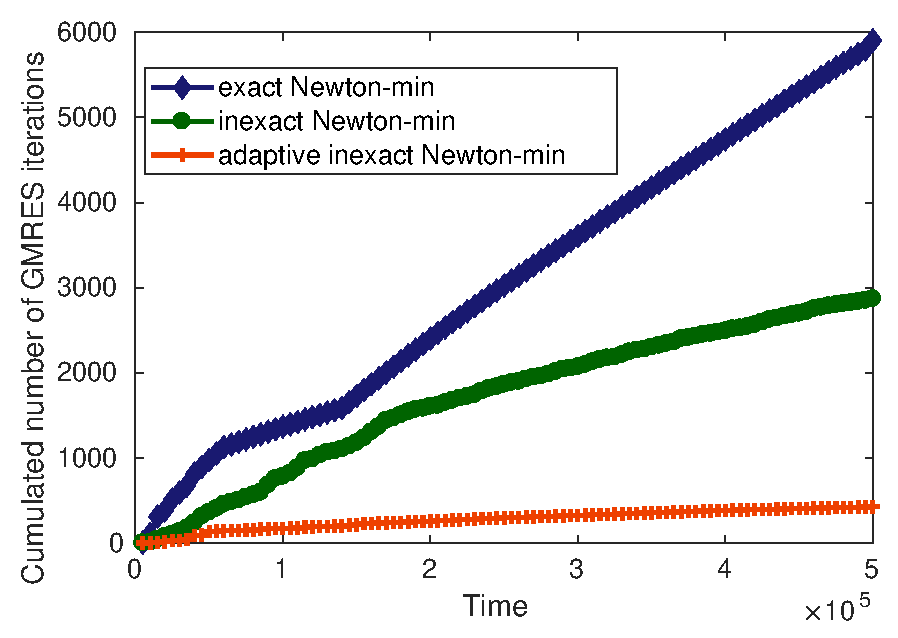
\includegraphics[width=0.44\textwidth]{image/Cumulated_number_gmres_iterations_three_methods_Nx_1000}
\end{figure}
\end{frame}
\begin{frame}
\frametitle{Accuracy}
\vspace{-0.1 cm}
\textcolor{cadmiumgreen}{$t = 1.05 \times 10^5$ years, $\gammalin = \gammaalg = 10^{-3}$} 
\vspace{-0.3 cm}
\begin{figure}
\centering
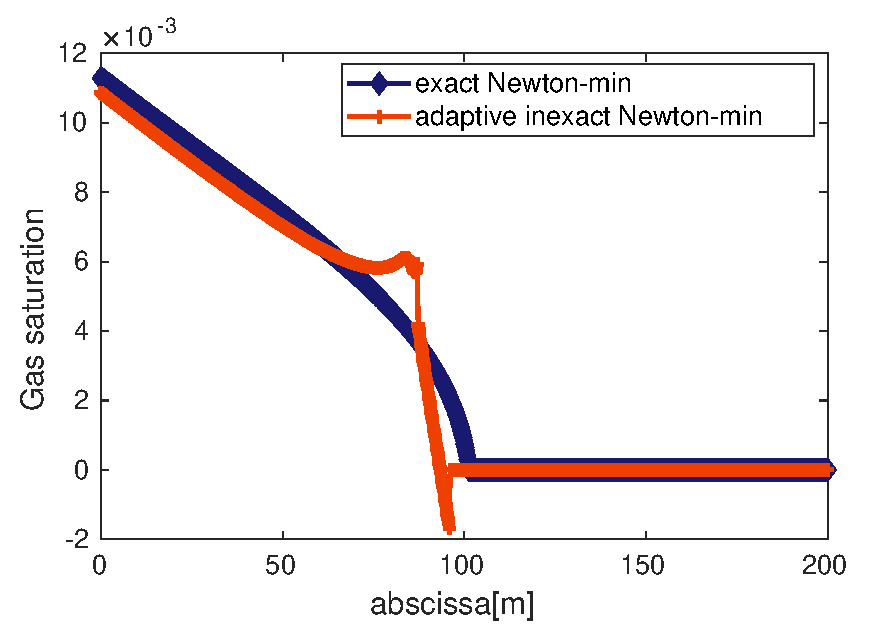
\includegraphics[width=0.40\textwidth]{image/comparaison_plot_gas_saturations_exact_adapt_inexact_gamma_lin_gamma_alg_10-3_nt_21}
%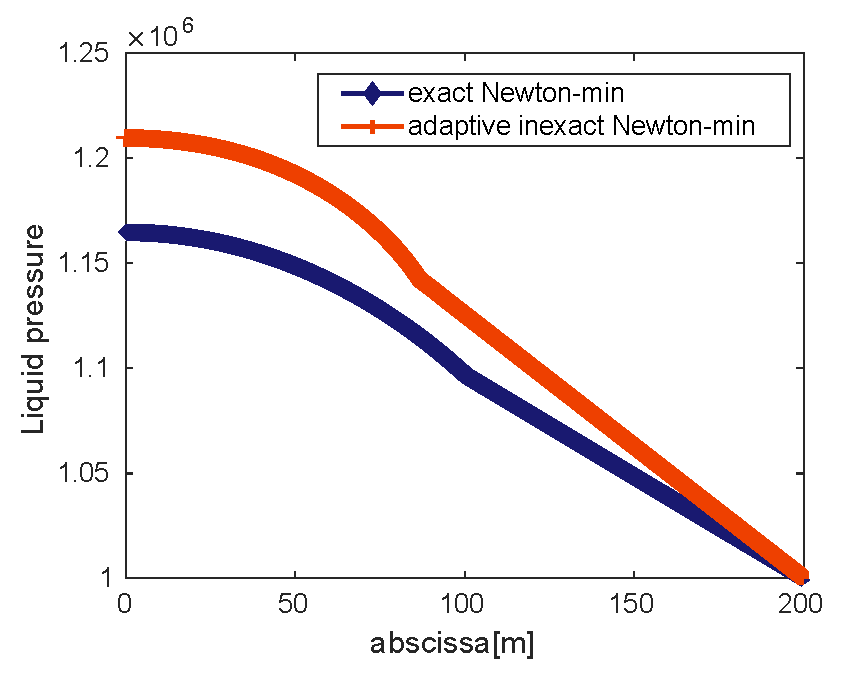
\includegraphics[width=0.31\textwidth]{image/MODIF_comparaison_plot_liq_pressure_exact_adapt_inexact_gamma_lin_gamma_alg_10-3_nt_21_TEST}
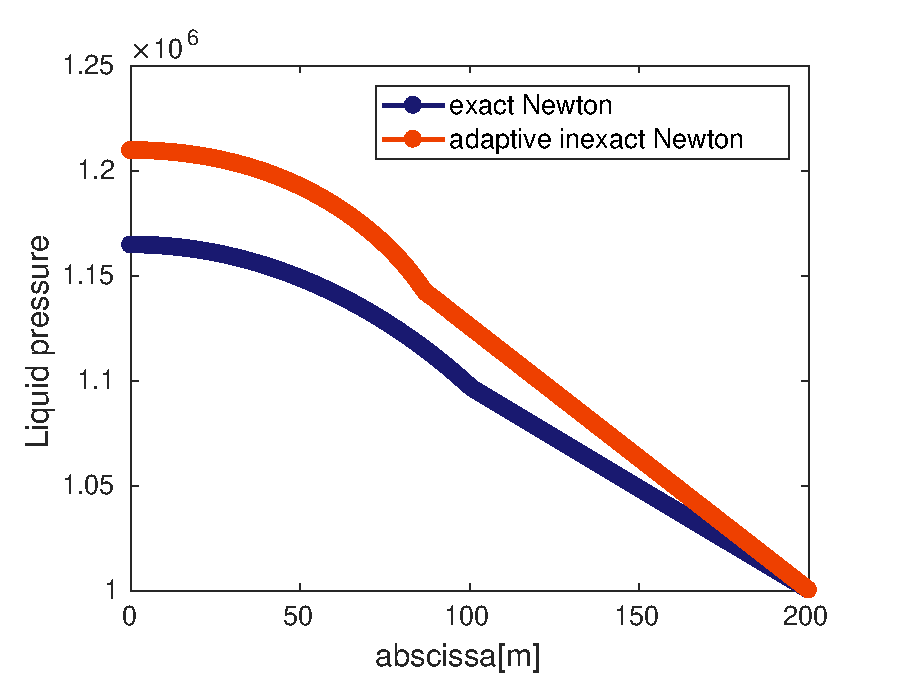
\includegraphics[width=0.4\textwidth]{image/comparaison_plot_liq_pressure_exact_adapt_inexact_gamma_lin_gamma_alg_10-3_nt_21}
\end{figure}
\vspace{-0.2 cm}
\textcolor{cadmiumgreen}{$t = 3.5 \times 10^5$ years, $\gammalin = \gammaalg = 10^{-3}$} 
\vspace{-0.3 cm}
\begin{figure}
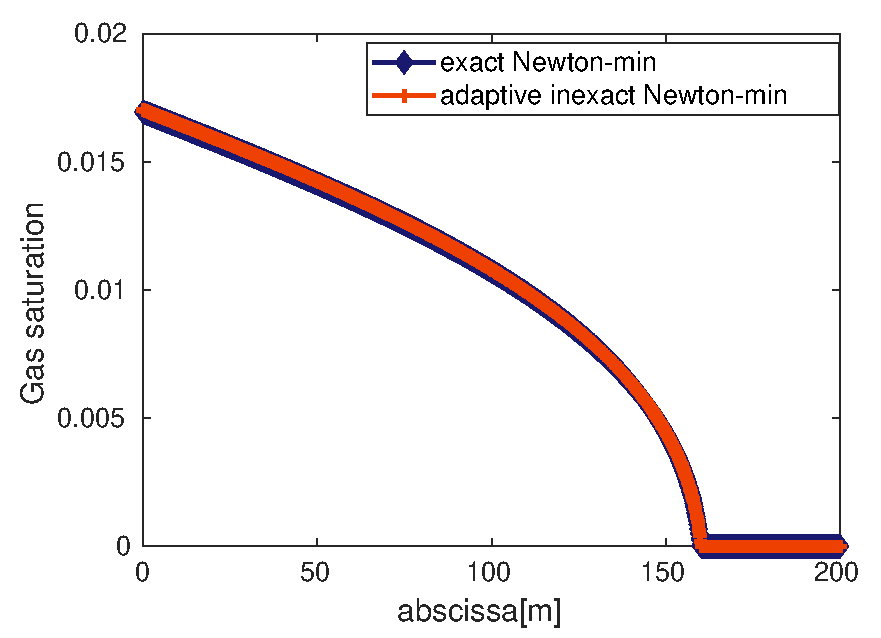
\includegraphics[width=0.40\textwidth]{image/comparaison_plot_gas_saturations_exact_adapt_inexact_gamma_lin_gamma_alg_10-3_nt_70}
%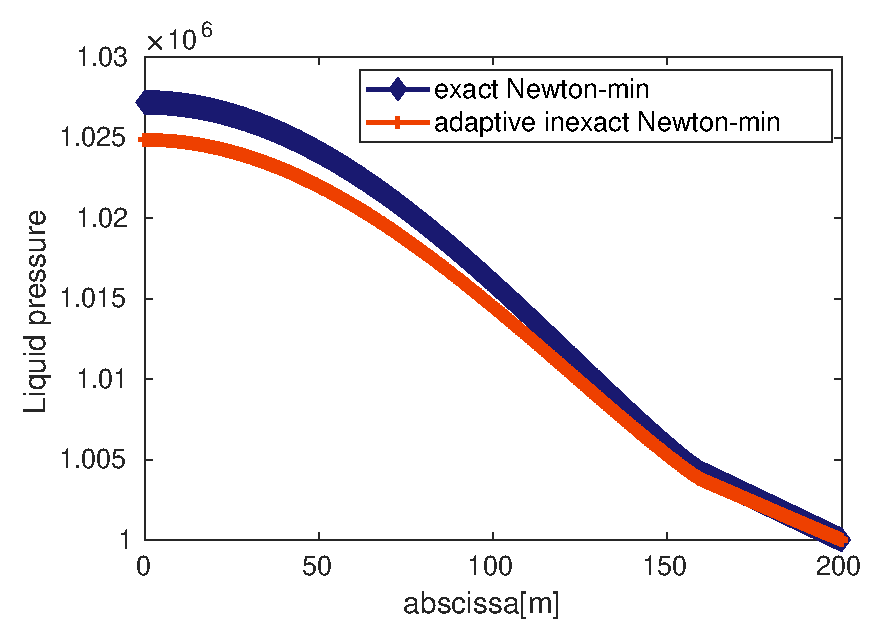
\includegraphics[width=0.33\textwidth]{image/comparaison_plot_liq_pressure_exact_adapt_inexact_gamma_lin_gamma_alg_10-3_nt_70}
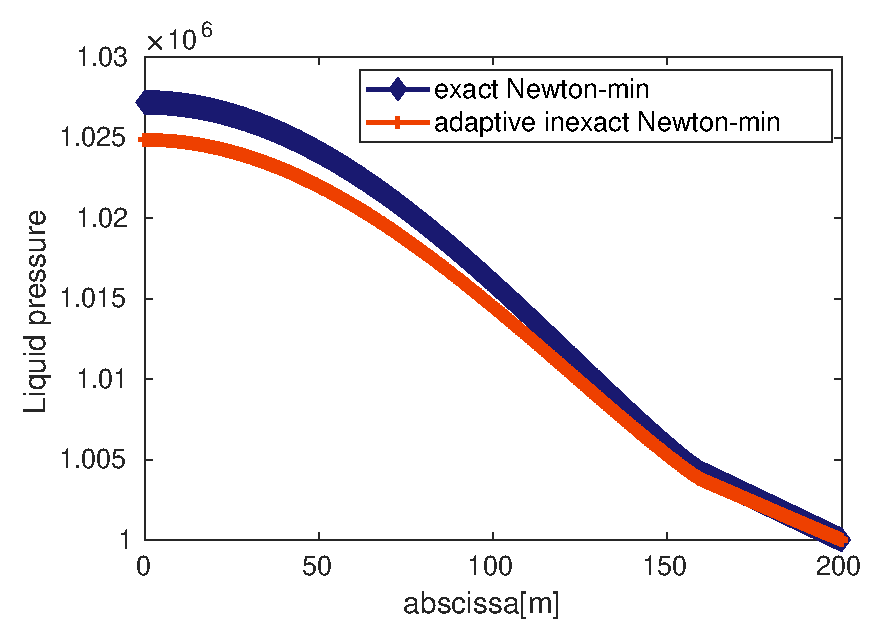
\includegraphics[width=0.41\textwidth]{image/comparaison_plot_liq_pressure_exact_adapt_inexact_gamma_lin_gamma_alg_10-3_nt_70}
\end{figure}
\end{frame}
%
\begin{frame}
\frametitle{Accuracy}
\textcolor{cadmiumgreen}{$t = 1.05 \times 10^5$ years, $\gammalin = 10^{-6}, \gammaalg = 10^{-3}$} 
\vspace{-0.2 cm}
\begin{figure}
\centering
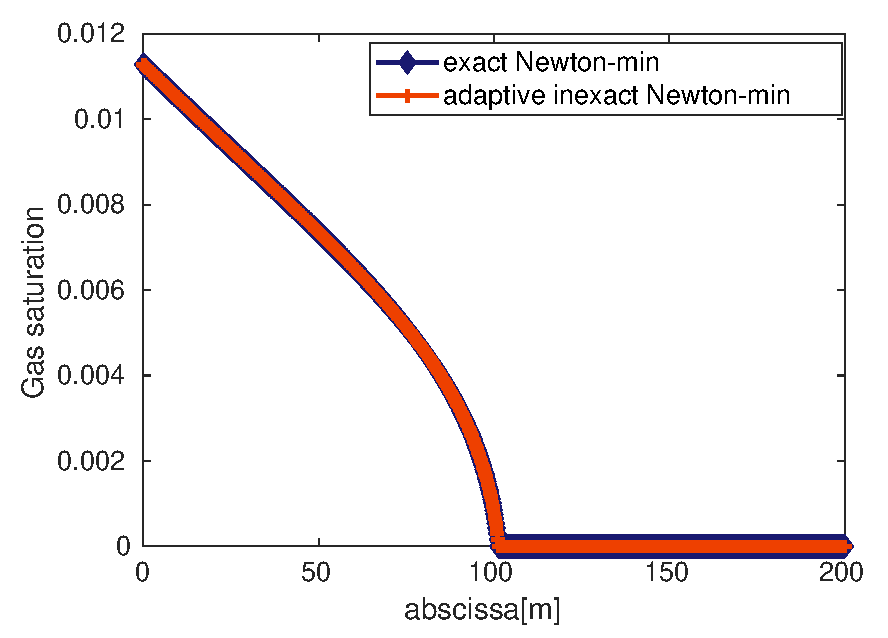
\includegraphics[width=0.47\textwidth]{image/comparaison_plot_gas_saturations_exact_adapt_inexact_gamma_lin_10-6_gamma_alg_10-3_nt_21}
\quad
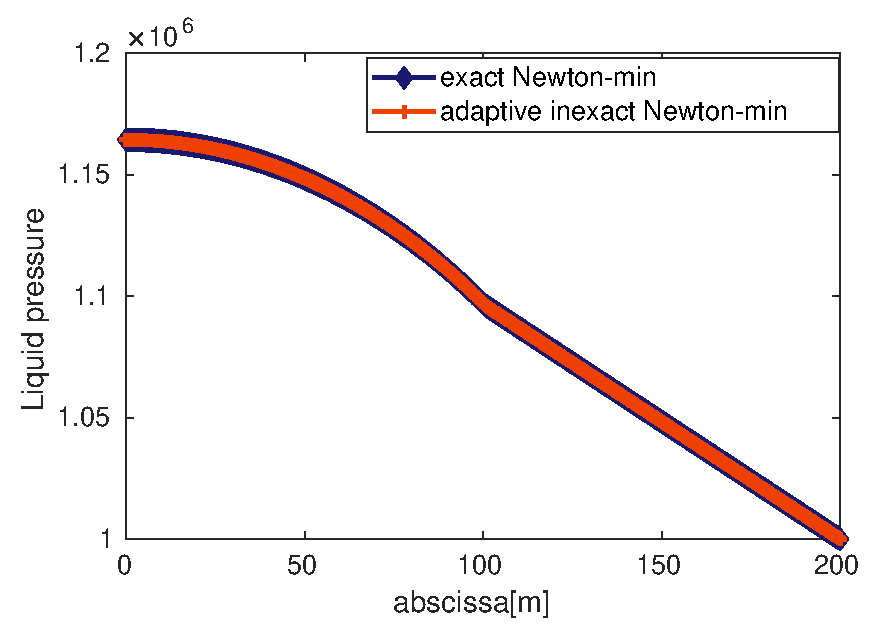
\includegraphics[width=0.48\textwidth]{image/comparaison_plot_liq_pressure_exact_adapt_inexact_gamma_lin_10-6_gamma_alg_10-3_nt_21}
\end{figure}
\vspace{-0.2 cm}
\scriptsize
\begin{table}
\centering
\begin{tabular}{lll}
\hline\noalign{\smallskip}
  $\left(\gammaalg,\gammalin\right)$ & \parbox{4.4 cm}{Cumulated Newton-min iterations} & \parbox{4.4 cm}{Cumulated GMRES iterations}  \\
\noalign{\smallskip}\hline\noalign{\smallskip}
($10^{-1},10^{-1}$)& 100 & 366 \\
($10^{-3}, 10^{-3}$) & 113  & 427 \\
($10^{-6},10^{-3}$) & 108 & 967 \\
($10^{-3},10^{-6}$) & 351 & 1682 \\
($10^{-6},10^{-6}$) & 308 & 2019 \\ 
Exact resolution & \textcolor{blue}{\textbf{600}} & \textcolor{blue}{\textbf{6000}}\\
\noalign{\smallskip}\hline
\end{tabular}
\end{table}
 
\end{frame}
\begin{frame}
\frametitle{Complements: Newton--Fischer--Burmeister}
\textcolor{cadmiumgreen}{
\begin{equation*}
%\label{eq:Fischer:Burmeister:function}
\left[\fFB (\ba, \bb)\right]_l = \sqrt{\ba_l^2 + \bb_l^2} - (\ba_l + \bb_l) \quad l=1,\ldots,\Nsp.
\end{equation*}
}
\scriptsize {\begin{table}
\centering
\begin{tabular}{lll}
\hline\noalign{\smallskip}
$\left(\gammaalg,\gammalin\right)$ & \hspace{-0.3 cm} \parbox{4.5 cm}{Cumulated number of Newton--Fischer--Burmeister iterations} &   \parbox{3.5 cm}{Cumulated number of GMRES  iterations}  \\
\noalign{\smallskip}\hline\noalign{\smallskip}
$\left(10^{-1},10^{-1} \right)$ & \qquad 100 & \quad \qquad 428 \\
$\left(10^{-3},10^{-3}\right)$ & \qquad 119 & \quad \qquad 751 \\
$\left(10^{-3},10^{-6}\right)$ & \qquad 482 & \quad \qquad 2074 \\
$\left(10^{-6},10^{-3}\right)$ & \qquad 117 & \quad \qquad 1694 \\
\textcolor{blue}{\textbf{Exact resolution}} & \qquad \textcolor{blue}{\textbf{757}} & \quad \hspace{0.2 cm} \quad \textcolor{blue}{\textbf{10089}} \\
\noalign{\smallskip}\hline
\end{tabular}
\end{table}
}

\normalsize
\begin{itemize}
\item[$\bullet$]  \textcolor{red}{\textbf{Adaptive inexact Newton--Fischer--Burmeister is faster than exact Newton--Fischer--Burmeister. It saves roughly $90 \%$  of the iterations}}
\item[$\bullet$] \textcolor{red}{\textbf{Adaptive inexact Newton-min is faster than Adaptive inexact Newton--Fischer--Burmeister. It saves roughly $40 \%$ of the iterations.}}
\end{itemize}. 

\end{frame}


\section{Conclusion}
\begin{frame}
\frametitle{Conclusion}
\begin{itemize}
\item
We devised an a posteriori error estimate between the exact and approximate solution for a wide class of semi-smooth Newton methods.
\vspace{0.5 cm}
\item 
This estimate distinguishes the error components.
\end{itemize}
\vspace{0.5 cm}
\textcolor{red}{\textbf{Ongoing work:}}
\begin{itemize}
\item
 Devise space-time adaptivity 
\item Optimize the code
\end{itemize}
\vspace{0.5 cm}
\begin{thebibliography}{10}
 \scriptsize{
 \bibitem{Dabaghi2:2018}
 {\sc I.~Ben Gharbia, J.~Dabaghi, V.~Martin, and M.~Vohral{\'{\i}}k}, {\em A posteriori error estimates and adaptive stopping criteria for a compositional two-phase flow with nonlinear complementarity constraints}.
 \textcolor{black}{HAL Preprint~01919067, submitted for publication, 2018}}

 \scriptsize{
 \bibitem{Dabaghi:2018}
 {\sc J.~Dabaghi, V.~Martin, and M.~Vohral{\'{\i}}k}, {\em Adaptive inexact
  semismooth Newton methods for the contact problem between two membranes}.
 \textcolor{black}{HAL Preprint~01666845, submitted for publication, 2018}
 }

 \scriptsize{
 \bibitem{Dabaghi3:2018}
 {\sc J.~Dabaghi, V.~Martin, and M.~Vohral{\'{\i}}k}, {\em A posteriori error estimate and adaptive stopping criteria for a parabolic variational inequality}.
 \textcolor{black}{In preparation.}
 }


 \end{thebibliography}


\end{frame}

\begin{frame}
\centering
\vspace*{1 cm}
\Huge Thank you for your attention!
\vspace*{2 cm}
\begin{figure}
\centering
\includegraphics[scale=1]{image/smiley}
\end{figure}
\end{frame}
%
%% %
%% %\begin{frame}
%% %\section{A posteriori and adaptivity}
%% %\subsection{A posteriori and adaptivity}
%% %\frametitle{A posteriori analysis and preliminary study}
%% %\alert{\textbf{A posteriori error estimates:}}
%% %$\dps |||\bu-\uhki||| \leq \left\{\dps \sum_{\substack{K \in\Th}} \eta_K(\uhki)^2\right\}^{1/2}$.\\
%% %
%% %%\alert{\textbf{Effectivity index:}} $\mathrm{I_{eff}}=\left\{\dps \sum_{\substack{K \in\Th}} \eta_K(\uhki)^2\right\}^{1/2} {\large /} \; {\dps|||\bu-\uhki|||} \quad \alert{\searrow 1} $ 
%% %%From \eqref{eq:modele_initial_membrane} if we define ${\bm \sigma}_1 = -\mu_1 \nab u_1$ and ${\bm \sigma}_2 = - \mu_2 \nab u_2$ we have $({\bm \sigma}_1,{\bm \sigma}_2) \in \HdivOmeg$,  and $\nab \cdot {\bm \sigma}_1 = f_1 + \lambda $ and $\nab \cdot {\bm \sigma}_2 = f_2 - \lambda $. \\\\
%% %%\includegraphics[scale=0.02]{attention} 
%% %%\footnotesize
%% %%$\left(-\nab \uunhki, -\nab \udeuxhki\right) \neq \HdivOmeg \hspace{0.1 cm}$  $\nab \cdot (- \mu_1 \nab \uunhki) \neq f_1 + \lambhki$  $\nab \cdot (-\mu_2 \nab \udeuxhki) \neq f_2 - \lambhki$.
%% %%\normalsize
%% %\scriptsize{
%% %\begin{thebibliography}{10}
%% %\bibitem{Repin:2008}
%% %Sergey Repin.
%% %\newblock {\em A posteriori estimates for partial differential equations}.
%% %\newblock Walter de Gruyter GmbH \& Co. KG, Berlin, 2008.
%% %\end{thebibliography}
%% %}
%% %
%% %\scriptsize{
%% %\begin{thebibliography}{10}
%% %\bibitem{Verfurth:2013}
%% %Verf\"urth, R\"udiger.
%% %\newblock {\em A posteriori error estimation techniques for finite element
%% %              methods}.
%% %\newblock Oxford University Press, 2013.
%% %\end{thebibliography}
%% %}
%% %
%% %\vspace{-0.3 cm}
%% %\normalsize
%% %\begin{equation*}
%% %\mbox{\textbf{Goal:}}\dps
%% %\left\lbrace\begin{array}{llccc}
%% %\dps \sigunhki \in \textbf H(\div,\Omega) \hspace{0.15 cm} \mbox{such that} \hspace{0.15 cm} (\nab \cdot \sigunhki,1)_K=(f_1+\lambhki,1)_K \hspace{0.15 cm} \forall K \in \Th, \\
%% %\dps\sigdeuxhki \in \textbf H(\div,\Omega) \hspace{0.15 cm} \mbox{such that} \hspace{0.15 cm} (\nab \cdot \sigdeuxhki,1)_K=(f_2-\lambhki,1)_K \hspace{0.15 cm} \forall K \in \Th .
%% %\end{array}
%% %\right.
%% %%\label{eq: 1.24}
%% %\end{equation*}
%% %\normalsize
%% %\begin{itemize}
%% %\item 
%% %$\sigunhki = \sigunhdiski + \sigunhalgki$ and $\sigdeuxhki = \sigdeuxhdiski + \sigdeuxhalgki$
%% %\end{itemize}
%% %
%% %%\textcolor{red}{\textbf{Assumption:}}
%% %%$\sigunhalgki+\sigunhdiski =\sigunhki$ and
%% %%$\sigdeuxhalgki+\sigdeuxhdiski =\sigdeuxhki$
%% %%\\
%% %\vspace{0.3 cm}
%% %\textcolor{red}{\textbf{Algebraic fluxes reconstruction:}}
%% %\begin{itemize}
%% %
%% %%$\lim\limits_{\substack{\textcolor{blue}{k},\textcolor{red}{i} \rightarrow + \infty}} {\left\|\sigunhalgki\right\|}_{L^2(\Omega)} = \lim\limits_{\substack{\textcolor{blue}{k},\textcolor{red}{i} \rightarrow + \infty }} {\left\|\sigdeuxhalgki\right\|}_{L^2(\Omega)} = 0$
%% %\item $\left\{\sigunhalgki,\sigdeuxhalgki\right\} \in \textbf H(\div,\Omega)$, \: $\nab \cdot \sigunhalgki=\runhki$, \: $\nab \cdot \sigdeuxhalgki=\rdeuxhki$
%% %\end{itemize}
%% %
%% %
%% %
%% %\scriptsize
%% %\begin{thebibliography}{10}
%% %  \bibitem{VorPapez:2015}
%% %Papez Jan, Rüde Ulrich, Vohral{\'{\i}}k Martin, and Wohlmuth Barbara.
%% %\newblock Sharp algebraic and total a posteriori error bounds via a multilevel
%% %approach.
%% %\newblock In preparation, 2017.
%% %\end{thebibliography}
%% %\end{frame}
%% %%\subsection{Discretization fluxes reconstruction}
%% %\begin{frame}
%% %\frametitle{Discretization fluxes reconstruction}
%% %%\subsection{Discretization flux reconstruction}
%% %%$\forall \ba \in \mathcal{V}_{h}$, define $(\sigunhdiskia,\sigdeuxhdiskia) \in {\bf V}_{h}^{\ba} \times {\bf V}_{h}^{\ba}$ and $(\gamunhkia,\gamdeuxhkia)\in Q_{h}^{\ba} \times Q_{h}^{\ba}$, where ${\bf V}_{h}^{\ba} \subset \textbf H(\div,\Omega)$ and $Q_{h}^{\ba} \subset L^2(\Omega)$ by solving:
%% %$\sigunhdiskia$ and $\sigdeuxhdiskia$ are the solution of mixed system on patches
%% %\begin{equation*}
%% %\left\lbrace\begin{array}{llccc}
%% %(\sigunhdiskia,{\bv}_{1h})_{\omega_{h}^{\ba}}-(\gamunhkia,\nab \cdot {\bv}_{1h})_{\omega_{h}^{\ba}} &=& \dps -\left(\psi_{h,\ba} \nab \uunhki,{\bv}_{1h}\right)_{\omega_h^{\ba}}  & \forall {\bv}_{1h}\in {\bf V}_{h}^{\ba}, \\
%% %\dps(\nab \cdot \sigunhdiskia,q_{1h})_{\omega_{h}^{\ba}}&=&\dps(\tildgunhkia,q_{1h})_{\omega_{h}^{\ba}} & \forall q_{1h}\in Q_{h}^{\ba},\\
%% %(\sigdeuxhdiskia,{\bv}_{2h})_{\omega_{h}^{\ba}}-(\gamdeuxhkia,\nab \cdot {\bv}_{2h})_{\omega_{h}^{\ba}} &=& \dps-\left(\psi_{h,\ba} \nab \udeuxhki,{\bv}_{2h}\right)_{\omega_h^{\ba}} & \forall {\bv}_{2h}\in {\bf V}_{h}^{\ba},\\
%% %(\nab \cdot \sigdeuxhdiskia,q_{2h})_{\omega_{h}^{\ba}}&=&\dps(\tildgdeuxhkia,q_{2h})_{\omega_{h}^{\ba}} & \forall q_{2h} \in Q_{h}^{\ba}.
%% %\end{array}
%% %\right.
%% %%\label{eq:reconstruction_flux_raviart_thomas:newton:min:inexacte:discretozation:flux}
%% %\end{equation*}
%% %%\begin{align*}
%% %%\tildgunhkia &=f_1 \psi_{h,\ba}- \mu_1 \nab \uunhki \cdot \nab \psi_{h,\ba} +\lambhki(\ba)\psi_{h,\ba} -\runhki \psi_{h,\ba} \quad \forall {\ba} \in \mathcal{V}_{h},\\
%% %%\tildgdeuxhkia &= f_2 \psi_{h,\ba}- \mu_2 \nab \udeuxhki \cdot \nab \psi_{h,\ba}-\lambhki(\ba)\psi_{h,\ba}-\rdeuxhki \psi_{h,\ba} \quad \forall {\ba} \in \mathcal{V}_h,
%% %%\end{align*}
%% %\hspace{1.2 cm}
%% %\fcolorbox{violet}{white}{
%% %\textcolor{black}{$\dps
%% %{{\sigunhdiski}}={\sum_{\ba \in \mathcal{V}_h} \sigunhdiskia} \quad \mbox{and} \quad \sigdeuxhdiski=\sum_{\ba \in \mathcal{V}_h} \sigdeuxhdiskia$}
%% %}
%% %\begin{itemize}
%% %\item
%% %$\sigunhdiski  \in \textbf H(\div,\Omega) \quad \mbox{and} \quad \left(\nab \cdot \sigunhdiski, 1\right)_K = \left(f_1 + \lambhki -\runhki ,1\right)_K$
%% %\item
%% %$\sigdeuxhdiski \in \textbf H(\div,\Omega) \quad \mbox{and} \quad \left(\nab \cdot \sigdeuxhdiski, 1\right)_K = \left(f_2 - \lambhki -\rdeuxhki ,1\right)_K$ .
%% %\end{itemize}
%% %
%% %
%% %\scriptsize{
%% %\begin{thebibliography}{10}
%% %\bibitem{Braess:2009}
%% %Braess, Dietrich and Pillwein, Veronika and Sch{\"o}berl,
%% %              Joachim.
%% %\newblock {\em Equilibrated residual error estimates are {$p$}-robust}.
%% %\newblock Computer Methods in Applied Mechanics and Engineering, 2009.
%% %\end{thebibliography}
%% %}
%% %
%% %\end{frame}
%% %%\subsection{A posteriori error estimates}
%% %\begin{frame}
%% %\frametitle{A posteriori error estimates}
%% %\vspace{-0.2 cm}
%% %
%% %\begin{itemize}
%% %\item
%% %${\bm u}=(u_1,u_2)\in\mathcal{K}_g$,\ $\uhki=(\uunhki,\udeuxhki)\in \mathbb{X}_{gh} \times \mathbb{X}_{0h}$,\ $\left\{\sigunhki, \sigdeuxhki\right\} \in \HdivOmeg$
%% %\end{itemize}
%% %\textcolor{red}{\textbf{Warning:}}
%% %$\uunhki(\ba) - \udeuxhki(\ba)$ and $\lambhki(\ba)$ can be negative. 
%% %%\vspace{-0.3 cm}
%% %\begin{figure}[H]
%% %\textcolor{red}{\hspace{-1.4 cm} \textbf{Example: k=2}}
%% %\begin{subfigure}[normal]{0.35\textwidth} 
%% %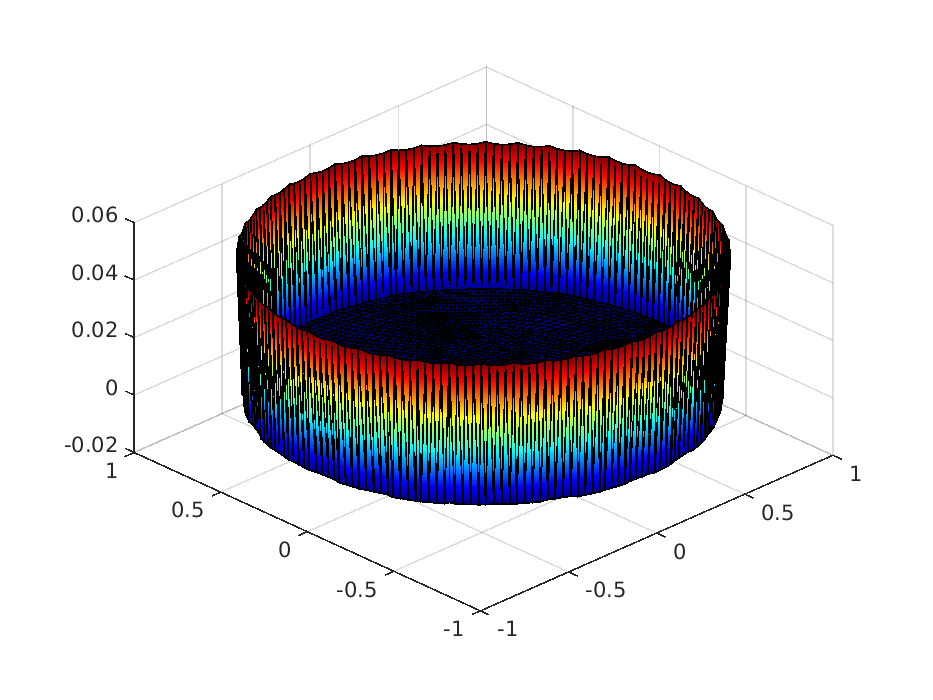
\includegraphics[width=\textwidth]{fig_article/diff_u1_u2_newton_gmres.eps}    
%% %\label{ref:position_membrane_inside_iter}
%% %\end{subfigure}
%% %\begin{subfigure}[normal]{0.35\textwidth}
%% %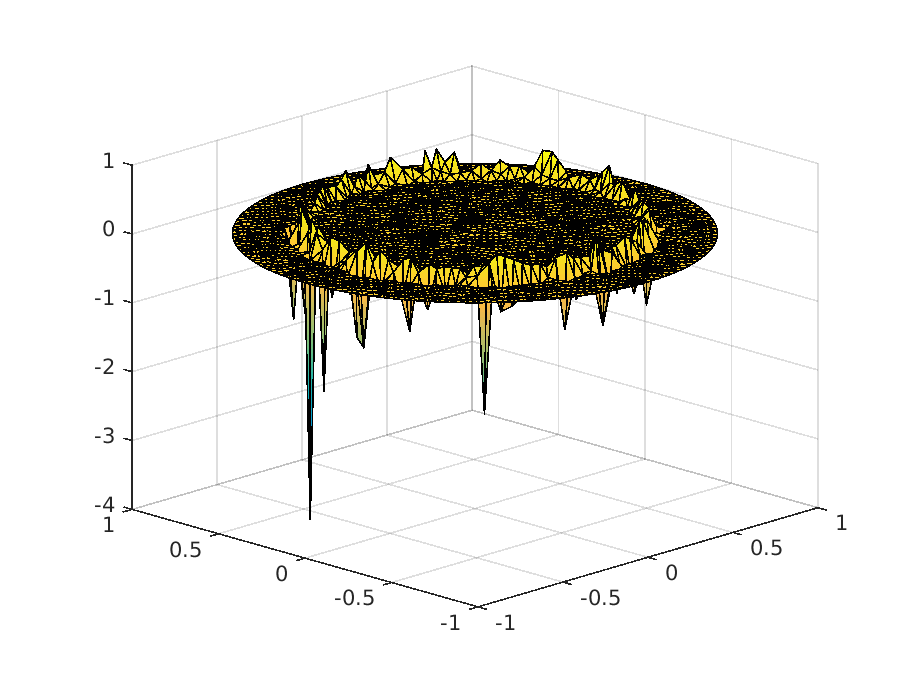
\includegraphics[width=\textwidth]{fig_article/lambda_newton_iter7.eps}     
%% %\label{ref:lambda_membrane_inside_iter} 
%% %\end{subfigure}
%% %%\caption{membranes (left) and lagrange multiplier (right) during the iterations }
%% %\end{figure}
%% %\vspace{-0.2 cm}
%% %\textcolor{cadmiumgreen}{\textbf{Motivation:}} Define $\shki \in \Kgh$ by
%% %\vspace{0.3 cm}
%% %$\dps \shki (\ba)= \dps \begin{cases}
%% %\uhki(\ba) = \left(\uunhki(\ba), \udeuxhki(\ba)\right) \quad &\mbox{if $\uunhki(\ba) \geq \udeuxhki(\ba)$,}\\
%% %\dps \left(\frac{\uunhki(\ba) + \udeuxhki(\ba)}{2}, \frac{\uunhki(\ba) + \udeuxhki(\ba)}{2}\right) \quad &\mbox{if $\uunhki(\ba) < \udeuxhki(\ba)$.}\end{cases}$
%% %\end{frame}
%% %\begin{frame}
%% %
%% %
%% %\begin{itemize}
%% %\item
%% %Discretization error estimators
%% %\vspace{0.3 cm}
%% %$\left.
%% %\begin{array}{ll}
%% %\dps {\eta}_{\mathrm{F},K,\ialf}^{\kk,\ii} &= \left\| \mu_\ialf^{\frac{1}{2}} \nab u_{\ialf h}^{\kk,\ii}+\mu_\ialf^{-\frac{1}{2}} \sigmaialfhdiscki \right\|_{K}  
%% %\\
%% %\dps {\eta}_{\mathrm{osc},K,\ialf} & =  \dps \frac{h_K}{\pi} \mu_\ialf^{-\frac{1}{2}} \left\|f_\ialf-{\bm \Pi}_{\mathbb{P}_1}(f_\ialf)\right\|_{K}\\
%% %\dps \etCKkipos & = 2 \dps \left(\uunhki-\udeuxhki,\lambhkipos\right)_K
%% %\end{array}
%% %\right\} \Rightarrow \dps {\bm \eta}^{\kk,\ii}_{\mathrm{disc}}
%% %$\\
%% %%\vspace{0.2 cm}
%% %\item
%% %Linearization error estimators
%% %\vspace{0.3 cm}
%% %%%%%%%%%%%
%% %$\left.
%% %\begin{array}{ll}
%% %\dps \etalinunKki  &=  \tnorm{\shki-\uhki}_K  
%% %\\
%% %\dps \etalindeuxKki &= 2 h_{\Omega} \CPF \left(\frac{1}{\mu_1} + \frac{1}{\mu_2} \right)^{\frac{1}{2}} \left\|\lambhkipos\right\|_{\Omega} \tnorm{\shki-\uhki}_K\\
%% %\dps \etalintroisKki &= h_{\Omega} \CPF \left(\frac{1}{\mu_1} + \frac{1}{\mu_2} \right)^{\frac{1}{2}} \left\| \lambhkineg\right\|_K
%% %\end{array}
%% %\right\} \Rightarrow \dps {\bm \eta}^{\kk,\ii}_{\mathrm{lin}}
%% %$
%% %\\
%% %\item
%% %Algebraic error estimators\\
%% %\vspace{0.1 cm}
%% %$\left.
%% %\begin{array}{ll}
%% %\dps \etaalgKialfki &= \left\|\mu_\ialf^{-\frac{1}{2}}\sigmaialfhalgki\right\|_{K}
%% %\end{array}
%% %\right\} \Rightarrow \dps {\bm \eta}^{\kk,\ii}_{\mathrm{alg}}
%% %$
%% %\end{itemize}
%% %
%% %\begin{theorem}[A posteriori  estimate distinguishing the error components]
%% %
%% %
%% %\emph{
%% %\textcolor{bulgarianrose}{
%% %\begin{equation*}
%% %\dps
%% %|||\bu-\uhki||| \leq \eta^{\kk,\ii}_{\mathrm{disc}} +\eta^{\kk,\ii}_{\mathrm{alg}} + \eta^{\kk,\ii}_{\mathrm{lin}}.
%% %\end{equation*}
%% %}}
%% %
%% %\end{theorem}
%% %\end{frame}
%% %
%% %\begin{frame}
%% %\vspace{-0.2 cm}
%% %\begin{proof}
%% %We define global versions of these estimators as $ \eta_{\cdot}^{k,i} = \left\{\sum_{K \in \Th}\left(\eta_{\cdot,K}^{k,i}\right)^2\right\}^{\frac{1}{2}}$
%% %\begin{enumerate}
%% %\item $\uhki \notin \Kgh$: define the projection 
%% %$\bs$ of $\uhki$ in $\Kg$ by $a(\bs,\bv-\bs) \geq a(\uhki,\bv-\bs) \quad \forall \bv \in \Kg $ \alert{Pb well posed: Lions-Stampacchia}
%% %
%% %
%% %\item<2-> 
%% %
%% %$
%% %\tnorm{\bu-\uhki}^2 = \underbrace{ a(\bu - \uhki, \bu - \bs)}_{=\textcolor{blue}{\textbf{A}}} + \underbrace{a(\bu  - \uhki, \bs-\uhki)}_{=\textcolor{cadmiumgreen}{\textbf{B}}}.
%% %%=a(\bu,\bu-\uhki)-a(\uhki,\bu-\uhki).
%% %$
%% %\item<3-> 
%% %
%% %$\textcolor{cadmiumgreen}{\textbf{B}} \leq \tnorm{\bu-\uhki} \etalinunki$
%% %\item<4-> 
%% %\footnotesize
%% %\vspace{-0.3 cm}
%% %$\dps
%% %\textcolor{blue}{\textbf{A}} \leq \left(\underbrace{\left\{\dps \sum_{K \in \Th}\dps \sum_{\ialf=1}^2({\eta}_{\mathrm{osc},K,\ialf} + {\eta}_{\mathrm{F},K,\ialf}^{\kk,\ii})^2\right\}^{\frac{1}{2}}}_{\textcolor{bulgarianrose}{\eta_1}} + \etalintroiski \right) \tnorm{\bu-\uhki} + \frac{1}{2} \etalindeuxki + \frac{1}{2} \sum_{K \in \Th} \etCKkipos 
%% %$
%% %\item<5-> 
%% %\alert{Young inequality:} $\dps \tnorm{\bu-\uhki} \leq  \left\{ \left(\eta_1^{\kk,\ii} + \etalinunki + \etalintroiski    \right)^2  + \etalindeuxki + \sum_K \etCKkipos \right\}^{\frac{1}{2}}.
%% %$
%% %\end{enumerate}
%% %\end{proof}
%% %\end{frame}
%% %
%% %%\begin{frame}
%% %%\scriptsize
%% %%$\dps \eta_1 \hspace{-0.1 cm} = \left\{\sum_{K \in \Th}\sum_{j=1}^2({\eta}_{\mathrm{R},K,j}^{k,i}+{\eta}_{\mathrm{F},K,j}^{k,i}+\etalgKjki)^2\right\}^{\frac{1}{2}}$ $\dps \eta_2 \hspace{-0.1 cm}= \left\{\sum_{K\in \Th} (\etLKkineg)^2\right\}^{\frac{1}{2}} \hspace{-0.2 cm} +\left\{\sum_{K\in \Th} (\etPKki)^2\right\}^{\frac{1}{2}}$
%% %%\\
%% %%\scriptsize
%% %%$\dps \eta_3 = \frac{1}{2} \sum_{K\in \Th}\left(\etCKkineg + \etCKkipos \right)+\left\{\sum_{K\in \Th} (\etLKkipos)^2\right\}^{\frac{1}{2}}$ 
%% %%$\dps \varepsilon_1 = \frac{1}{2} \hspace{-0.1 cm} + \frac{1}{2}\frac{\min(1, \eta_2)}{\eta_2}$  $\dps \varepsilon_2 \hspace{-0.1 cm}=\min(\frac{1}{2}, \eta_2)$
%% %%\vspace{-0.2 cm}
%% %%\normalsize
%% %
%% %%\begin{itemize}
%% %%\item 
%% %%$\dps \eta^{k,i}_{\mathrm{disc}} = \sqrt{2} \left\{3 \sum_{j=1}^{2}\left(\sum_{K \in \Th} \left({\eta}_{\mathrm{R},K,j}^{k,i} + {\eta}_{\mathrm{F},K,j}^{k,i}\right)^{2}\right) + \frac{1}{2} \sum_{K \in \Th} \etCKkipos \right\}^{\frac{1}{2}}$
%% %%\item
%% %%$\dps \eta^{k,i}_{\mathrm{alg}} =  \sqrt{6} \left\{\sum_{j=1}^{2} \sum_{K \in \Th} \left(\etalgKjki\right)^{2}\right\}^{\frac{1}{2}}$
%% %%\item
%% %%$\dps \eta^{k,i}_{\mathrm{lin}} = \sqrt{2} \left\{\sum_{K \in \Th} \left(2 \left(\etLKkineg + \etPKki\right)^2 + \frac{1}{2} \etCKkineg + \etLKkipos\right)\right\}^{\frac{1}{2}}$
%% %%\end{itemize}
%% %
%% %%\end{frame}
%% %%\section{Adaptive Inexacte semi-smooth Newton method}
%% %
%% %%%%%%%%%%%%%%%%%%%%%%%ADAPTIVE ALGORITHM IF FOR
%% %%\begin{frame}
%% %%\frametitle{Adaptive inexacte semi-smooth Newton algorithm}
%% %%%\vspace{-0.3 cm}
%% %%\vspace{-0.4 cm}
%% %%\begin{algorithm}[H]
%% %%\caption{Adaptive inexact semi-smooth Newton algorithm}
%% %%
%% %%\begin{algorithmic}
%% %%\STATE{\textbf{Initialization:}\; Choose an initial vector $\Xh^{\textcolor{royalblue}{0}} \in \mathcal{M}_{3N_h,1}(\R)$}
%% %%\FOR{$\textcolor{royalblue}{k=1 : N_{\mathrm{newton}}^{\mathrm{max}}}$} 
%% %%\STATE {Compute $\A^{\textcolor{royalblue}{k-1}} \hspace{-0.1
%% %% cm} \in \mathcal{M}_{3N_h,3N_h}(\R)$, $\bB^{\textcolor{royalblue}{k-1}} \hspace{-0.1 cm} \in \mathcal{M}_{3N_h,1}(\R)$ \\
%% %%Consider 
%% %%%the system of linear algebraic equations 
%% %%$\A^{\textcolor{royalblue}{k-1}} \Xhk= \bB^{\textcolor{royalblue}{k-1}}$}
%% %%\STATE{\textbf{Initialization for the linear solver:} Define $\X_h^{\kk,\textcolor{burntorange}{0}} = \X_h^{\textcolor{royalblue}{k-1}}$ 
%% %%%as initial guess for the linear solver 
%% %%}
%% %%	\FOR{$\textcolor{burntorange}{i=1 : N_{\mathrm{alg}}^{\mathrm{max}}}$}\STATE Compute Residual: {$\Rhki =\bB^{\textcolor{royalblue}{k-1}}-\A^{\textcolor{royalblue}{k-1}} \Xhki$}\\
%% %%	Compute estimators 
%% %%	\IF{\fcolorbox{violet}{white}{$\eta_{\mathrm{alg}}^{\kk,\ii} \leq \gamma_{\mathrm{alg}} \max  \left\{{\eta_{\mathrm{disc}}^{\kk,\ii}, \eta_{\mathrm{lin}}^{\kk,\ii}}\right\}$}} \STATE {Set $\Xhk = \Xhki$ end of linear solver (\textbf{break})} 
%% %%	%\ELSE \STATE{$\ii=\ii+1$}
%% %%	\ENDIF
%% %%	\ENDFOR
%% %%	\IF{\fcolorbox{violet}{white}{$\eta_{\mathrm{lin}}^{\kk,\ii} \leq \gamma_{\mathrm{lin}} \eta_{\mathrm{disc}}^{\kk,\ii}$}} \STATE {Set $\Xhk = \Xh$, end of non linear solver (\textbf{return})} 
%% %%%	\ELSE \STATE{$\kk=\kk+1$} 
%% %%\ENDIF
%% %%\ENDFOR
%% %%\end{algorithmic}
%% %%\end{algorithm}
%% %%\scriptsize
%% %%\vspace{-0.4 cm}
%% %%%\begin{thebibliography}{10}
%% %%%\bibitem{VorErn:2013}
%% %%%Alexandre Ern and Martin Vohral{\'{\i}}k.
%% %%%\newblock Adaptive inexact {N}ewton methods with a posteriori stopping criteria
%% %%%  for nonlinear diffusion {PDE}s. {\em SIAM J. Sci. Comput.}, 35(4):A1761--A1791, 2013.
%% %%%\end{thebibliography}
%% %%\end{frame}
%% %%\begin{frame}
%% %%\scriptsize
%% %%\vspace{-0.3 cm}
%% %%\begin{algorithm}[H]
%% %%\caption{Adaptive Inexact semi-smooth Newton algorithm}
%% %%\begin{algorithmic}
%% %%\STATE $ {\bm 1.} \hspace{0.1 cm} \mbox{Choose an initial vector $\Xh^{0} \in \mathcal{M}_{3N_h,1}(\R)$ \hspace{0.15 cm} and we set $\kk=1$}.$\\
%% %%\vspace{0.1 cm}
%% %%\STATE $ {\bm 2.} \hspace{0.1 cm} \mbox{From $\Xh^{k-1}$ define $\A^{\kk-1} \in \mathcal{M}_{3N_h,3N_h}(\R)$ and $\mathbb{F}^{\kk-1} \in \mathcal{M}_{3N_h,1}(\R)$.}$\\
%% %%\vspace{0.1 cm}
%% %%\STATE  $ {\bm 3.}\hspace{0.1 cm} \mbox{Consider the system of linear algebraic equations $\A^{\kk-1} \Xhk= \mathbb{F}^{\kk-1}$ ($*$)}$.\\
%% %%\vspace{0.1 cm}
%% %%\STATE  ${\bm {3a}.} \hspace{0.1 cm} \mbox{Define $\X_h^{\kk,0} = \X_h^{k-1}$ as initial guess for the linear solver and set $\ii=0$}$.\\
%% %%\vspace{0.1 cm}
%% %%\STATE  ${\bm {3b}.}\hspace{0.1 cm}  \mbox{For $\textcolor{red}{\ii}>0$ the approximation $\Xhki$ to $\Xhk$ satisfy $\A^{\kk-1} \Xhki +\Rhki =\mathbb{F}^{\kk-1}$ ($**$)}$.\\
%% %%\vspace{0.1 cm}
%% %%\STATE ${\bm 4.}\hspace{0.1 cm} \mbox{\textcolor{cadmiumgreen}{\textbf{Adaptive inexact resolution for ($**$)}}}$.\\
%% %%\vspace{0.1 cm}
%% %%\STATE $\qquad {\bm {4a}.} \hspace{0.1 cm} \mbox{Stopping criterion for the linear solver: $\eta_{\mathrm{alg}}^{\kk,\ii} \leq \gamma_{\mathrm{alg}} \max \left\{\eta_{\mathrm{disc}}^{\kk,\ii}, \eta_{\mathrm{lin}}^{\kk,\ii}\right\}$.}$
%% %%\vspace{0.1 cm}
%% %%\STATE $ \qquad \mbox{If satisfied, set $\Xhk = \Xhki$. If not, set $\ii=\ii+1$ and go back to $(**)$.}$\\
%% %%\vspace{0.1 cm}
%% %%\STATE $\qquad {\bm {4b}.}\hspace{0.1 cm}  \mbox{Sopping criterion for the non linear solver: $\eta_{\mathrm{lin}}^{\kk,\ii} \leq \gamma_{\mathrm{lin}} \eta_{\mathrm{disc}}^{\kk,\ii}$.}$\\
%% %%\vspace{0.1 cm}
%% %%\STATE $\qquad \mbox{If satisfied finish. If not, set $\kk=\kk+1$ and go back to ${\bm 2}.$}$
%% %%\label{ref:adpative:exact:inexacte algorithm}
%% %%\end{algorithmic}
%% %%\label{ref:methode_newton_min_exacte}
%% %%\end{algorithm}
%% %%\scriptsize
%% %%\begin{thebibliography}{10}
%% %%\bibitem{VorErn:2013}
%% %%Alexandre Ern and Martin Vohral{\'{\i}}k.
%% %%\newblock Adaptive inexact {N}ewton methods with a posteriori stopping criteria
%% %%  for nonlinear diffusion {PDE}s. {\em SIAM J. Sci. Comput.}, 35(4):A1761--A1791, 2013.
%% %%\end{thebibliography}
%% %%\end{frame}
%% %
%% %%%%%%%%%%ALGO LIKE PAPER MARTIN SIAM
%% %%%%%%%%%%%%%%%
%% %%\scriptsize
%% %%\begin{algorithmic}
%% %%\STATE $ {\bm 1.} \hspace{0.1 cm} \mbox{Choose an initial vector $\Xh^{0} \in \mathcal{M}_{3N_h,1}(\R)$ \hspace{0.15 cm} and we set $k=1$}.$\\
%% %%\STATE $ {\bm 2.} \hspace{0.1 cm} \mbox{From $\Xh^{k-1}$ define the matrix $\A^{k-1} \in \mathcal{M}_{3N_h,3N_h}(\R)$ and the vector $\mathbb{F}^{k-1} \in \mathcal{M}_{3N_h,1}(\R)$  by \eqref{eq:def:jac_clarke:A:right:hand:side:newton:newton}.}$\\
%% %%\STATE  $ {\bm 3.}\hspace{0.1 cm} \mbox{Consider the system of linear algebraic equations $\A^{k-1} \Xhk= \mathbb{F}^{k-1}$ ($*$)}$.\\
%% %%\STATE  ${\bm {3a}.} \hspace{0.1 cm} \mbox{Define $\X_h^{k,0} = \X_h^{k-1}$ as initial guess for the iterative linear solver and set $i=0$}$.\\
%% %%\STATE  ${\bm {3b}.}\hspace{0.1 cm}  \mbox{Perform $\nu$ steps of a chosen iterative lienar solver for the solution of the linear system $(*)$ starting}$\\
%% %%\STATE $\mbox{from the vector $\Xhki$. This yields on step $i \geq 0$ an approximation $\Xhki$ to $\Xhk$ satisfying}$\\
%% %%\STATE$\mbox{$\A^{k-1} \Xhki +\Rhki =\mathbb{F}^{k-1}$ ($**$)}$.\\
%% %%\STATE ${\bm 4.}\hspace{0.1 cm} \mbox{\textcolor{blue}{Exact resolution for ($**$)}}$.\\
%% %%\only<2>{
%% %%\STATE $\qquad {\bm {4a}.}\hspace{0.1 cm}  \mbox{Check the stopping criterion for the linear solver in the form $\left\|\bR_{\mathrm{alg}} \right\| \leq \varepsilon_1$}$.\\
%% %%\STATE $ \qquad\mbox{If satisfied, set $\Xhk = \Xhki$. If not, set $i=i+\nu$ and go back to ${\bm 3b}$.}$\\
%% %%\STATE $\qquad {\bm {4b}.}\hspace{0.1 cm}  \mbox{Check the stopping criterion for the non linear solver in the form $\left\|\bR_{\mathrm{lin}} \right\| \leq \varepsilon_1$}$.\\
%% %%\STATE $ \qquad\mbox{If satisfied finish. If not, set $k=k+1$ and go back to ${\bm 2}.$}$\\}
%% %%\STATE ${\bm 5.}\hspace{0.1 cm} \mbox{\textcolor{cadmiumgreen}{Inexact resolution for ($**$)}}$.\\
%% %%\only<3>{\STATE $\qquad {\bm {5a}.}\hspace{0.1 cm} \mbox{Check the stopping criterion for the linear solver in the form $\left\|\bR_{\mathrm{alg}} \right\| \leq \alpha_{\mathrm{alg}}\left\|\bR_{\mathrm{lin}} \right\|$}$.\\
%% %%\STATE $ \qquad\mbox{If satisfied, set $\Xhk = \Xhki$. If not, set $i=i+\nu$ and go back to ${\bm {3b}}$}$.\\
%% %%\STATE $\qquad {\bm {5b}.} \hspace{0.1 cm} \mbox{Check the stopping criterion for the non linear solver in the form $\left\|\bR_{\mathrm{lin}} \right\| \leq \varepsilon_1$}$.\\
%% %%\STATE $ \qquad\mbox{If satisfied finish. If not, set $k=k+1$ and go back to ${\bm 2}.$}$\\
%% %%}
%% %%\STATE ${\bm 6.}\hspace{0.1 cm} \mbox{\textcolor{red}{Adaptive inexact resolution for ($**$)}}$.\\
%% %%\only<4>
%% %%{
%% %%\STATE $\qquad {\bm {6a}.} \hspace{0.1 cm} \mbox{Check the stopping criterion for the linear solver in the form $\eta_{\mathrm{alg}}^{k,i} \leq \gamma_{\mathrm{alg}} \max \left\{\eta_{\mathrm{disc}}^{k,i}, \eta_{\mathrm{lin}}^{k,i}\right\}$.}$
%% %%\STATE $ \qquad \mbox{If satisfied, set $\Xhk = \Xhki$. If not, set $i=i+1$ and go back to $(**)$.}$\\
%% %%\STATE $\qquad {\bm {6b}.}\hspace{0.1 cm}  \mbox{Check the stopping criterion for the non linear solver in the form $\eta_{\mathrm{lin}}^{k,i} \leq \gamma_{\mathrm{lin}} \eta_{\mathrm{disc}}^{k,i}$.}$\\
%% %%\STATE $\qquad \mbox{If satisfied finish. If not, set $k=k+1$ and go back to ${\bm 2}.$}$
%% %%}
%% %%\label{ref:adpative:exact:inexacte algorithm}
%% %%\end{algorithmic}
%% %%\label{ref:methode_newton_min_exacte}
%% %%\end{algorithm}
%% %%\end{frame}
%% %
%% %\begin{frame}
%% %\vspace{-0.3 cm}
%% %\begin{algorithm}[H]
%% %\frametitle{Adaptive inexacte semi-smooth Newton algorithm}
%% %\caption{Adaptive inexact semi-smooth Newton algorithm}
%% %\begin{algorithmic}
%% %
%% %\STATE{\textbf{Initialization:}\; Choose an initial vector $\Xh^{\textcolor{royalblue}{0}} \in \mathcal{M}_{3N_h,1}(\R)$, ($\kk=0$)}\\
%% %\STATE{\textbf{Do}}\\
%% %\STATE{\quad$\kk =\textcolor{royalblue}{k+1}$}\\
%% %\STATE {\quad Compute $\A^{\textcolor{royalblue}{k-1}} \hspace{-0.1
%% % cm} \in \mathcal{M}_{3N_h,3N_h}(\R)$, $\bB^{\textcolor{royalblue}{k-1}} \hspace{-0.1 cm} \in \mathcal{M}_{3N_h,1}(\R)$ \\
%% %\quad Consider 
%% %%the system of linear algebraic equations 
%% %$\A^{\textcolor{royalblue}{k-1}} \Xhk= \bB^{\textcolor{royalblue}{k-1}}$}
%% %\STATE{\quad \textbf{Initialization for the linear solver:} Define $\X_h^{\kk,\textcolor{burntorange}{0}} = \X_h^{\textcolor{royalblue}{k-1}}$, ($\textcolor{burntorange}{i=0}$) 
%% %%as initial guess for the linear solver 
%% %}\\
%% %\STATE{\quad \textbf{Do}}
%% %	\STATE{\qquad $\textcolor{burntorange}{i=i+1}$}\\	
%% %	\STATE \qquad Compute Residual: {$\Rhki =\bB^{\textcolor{royalblue}{k-1}}-\A^{\textcolor{royalblue}{k-1}} \Xhki$}\\
%% %	\qquad  Compute estimators 
%% %	\STATE{\quad \textbf{While} \fcolorbox{violet}{white}{$\eta_{\mathrm{alg}}^{\kk,\ii} \geq \gamma_{\mathrm{alg}} \max  \left\{{\eta_{\mathrm{disc}}^{\kk,\ii}, \eta_{\mathrm{lin}}^{\kk,\ii}}\right\}$}} 
%% %	
%% %	
%% %	
%% %	\STATE{\textbf{While} \fcolorbox{violet}{white}{ $\eta_{\mathrm{lin}}^{\kk,\ii} \geq \gamma_{\mathrm{lin}} \eta_{\mathrm{disc}}^{\kk,\ii}$}} 
%% %	\STATE{\textbf{End}}
%% %%	\ELSE \STATE{$\kk=\kk+1$} 
%% %
%% %\end{algorithmic}
%% %\end{algorithm}
%% %\end{frame}
%% %
%% %
%% %
%% %
%% %\begin{frame}
%% %\section{Numerical experiments}
%% %\subsection{Numerical experiments}
%% %
%% %\frametitle{Numerical experiments}
%% %
%% %\begin{itemize}
%% %\item
%% %$\Omega$ = \mbox{unit disk}, $J = 3$, $\mu_1= \mu_2 = 1$, $g = 0.05$, $\gamma_{\mathrm{lin}}=0.3$ $\gamma_{\mathrm{alg}}=0.3$
%% %\item 
%% %Semi-smooth solver: \textcolor{blue}{Newton-min}. Linear solver: \textcolor{red}{GMRES}
%% %\end{itemize}
%% %
%% %
%% %\begin{figure}
%% %\begin{minipage}[c]{.33\linewidth}
%% %   \centering
%% %   Exact Newton
%% %\includegraphics[width=\textwidth]{image_article_membrane_version_Juillet_2017/modif_exact_resolution_convergence_estimator_number_elements.eps}    
%% %%\label{ref:position_membrane_convergence}
%% %\end{minipage}\hfill
%% %\begin{minipage}[c]{.33\linewidth}
%% %   \centering
%% %   Inexact Newton
%% %\includegraphics[width=\textwidth]{image_article_membrane_version_Juillet_2017/modif_inexact_resolution_convergence_estimator_number_elements.eps}    
%% %%\label{ref:position_membrane_convergence}
%% %\end{minipage}\hfill
%% %\begin{minipage}[c]{.33\linewidth}
%% %   \centering
%% %   Adaptive inexact Newton
%% %\includegraphics[width=\textwidth]{image_article_membrane_version_Juillet_2017/modif_adapt_inexact_resolution_convergence_estimator_number_elements.eps}     
%% %%\label{ref:lambda_membrane_convergence} 
%% %\end{minipage}
%% %%\caption{Exact Newton(left), Inexact Newton(middle), adaptive inexact Newton(right)}
%% %\end{figure}
%% %
%% %\textcolor{red}{\textbf{Quality and precision are preserved for adaptive inexact semi-smooth Newton method.}}
%% %
%% %
%% %\end{frame}
%% %
%% %\begin{frame}
%% %\begin{figure}
%% %\begin{minipage}[c]{.33\linewidth}
%% %   \centering
%% %   Exact Newton
%% %\includegraphics[width=\textwidth]{image_article_membrane_version_Juillet_2017/modif_exact_resolution_estimators_gmres_iter_inside_first_newton_iter_Hmax_015.eps}    
%% %%\label{ref:position_membrane_convergence}
%% %\end{minipage}\hfill
%% %\begin{minipage}[c]{.33\linewidth}
%% %   \centering
%% %   Inexact Newton
%% %\includegraphics[width=\textwidth]{image_article_membrane_version_Juillet_2017/modif_inexacte_resolution_Hmax_015_number_gmres_iter_inside_first_newton_step.eps}    
%% %%\label{ref:position_membrane_convergence}
%% %\end{minipage}\hfill
%% %\begin{minipage}[c]{.33\linewidth}
%% %   \centering
%% %   Adaptive inexact Newton
%% %\includegraphics[width=\textwidth]{image_article_membrane_version_Juillet_2017/modif_adapt_inexact_resolution_estimators_gmres_iter_inside_first_newton_iter_Hmax_015.eps}     
%% %%\label{ref:lambda_membrane_convergence} 
%% %\end{minipage}
%% %%\caption{Exact Newton(left), Inexact Newton(middle), adaptive inexact Newton(right)}
%% %\end{figure}
%% %
%% %\vspace{-0.3 cm}
%% %\begin{figure}
%% %   \begin{minipage}[c]{.33\linewidth}
%% %   \centering
%% %   Exact  Newton 
%% %\includegraphics[width=\textwidth]{image_article_membrane_version_Juillet_2017/modif_exact_resolution_estimators_newton_iter_Hmax_015.eps}    
%% %   \end{minipage} \hfill
%% %   \begin{minipage}[c]{.33\linewidth}
%% %   \centering
%% %   Inexact Newton
%% %\includegraphics[width=\textwidth]{image_article_membrane_version_Juillet_2017/modif_inexacte_resolution_Hmax_015_estimators_newton_step.eps}     
%% %   \end{minipage} \hfill
%% %  \begin{minipage}[c]{.32\linewidth}
%% %  \centering
%% %  Adaptive Inexact Newton  
%% %   \includegraphics[width=\textwidth]{image_article_membrane_version_Juillet_2017/modif_adapt_inexact_resolution_estimators_newton_iter_Hmax_015.eps}     
%% %\end{minipage}\hfill
%% %\end{figure}
%% %\end{frame}
%% %
%% %
%% %%
%% %%\begin{figure}[H]
%% %%\begin{subfigure}[normal]{0.32\textwidth} 
%% %%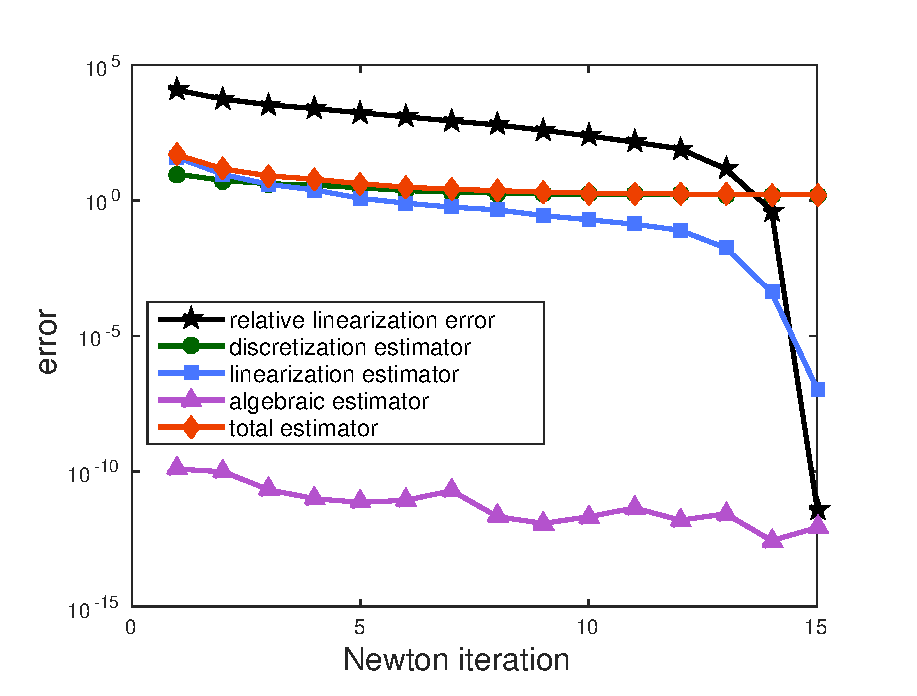
\includegraphics[width=\textwidth]{fig_article/estimators_newton_step_exact_resolution.eps}    
%% %%%\label{ref:position_membrane_convergence}
%% %%\end{subfigure}
%% %%\begin{subfigure}[normal]{0.32\textwidth}
%% %%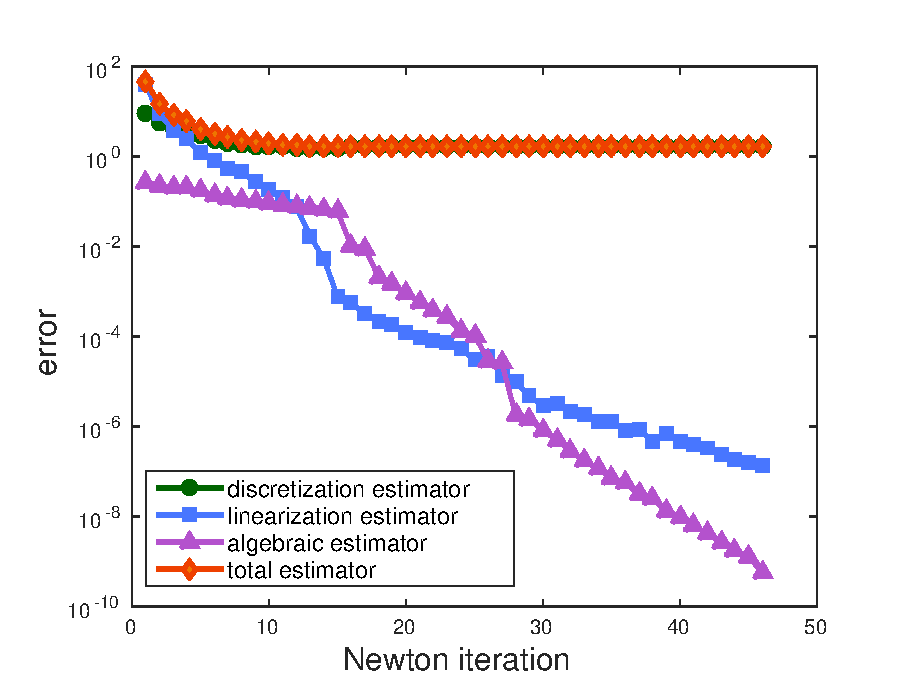
\includegraphics[width=\textwidth]{fig_article/estimators_newton_step_inexact_resolution.eps}     
%% %%%\label{ref:lambda_membrane_convergence} 
%% %%\end{subfigure}
%% %%\begin{subfigure}[normal]{0.33\textwidth}
%% %%\includegraphics[width=\textwidth]{fig_article/estimators_newton_step_adapt_inexact_resolution.eps}     
%% %%%\label{ref:lambda_membrane_convergence} 
%% %%\end{subfigure}
%% %%\caption{Exact Newton(left), inexact Newton(middle), adaptive inexacte Newton(right)}
%% %%\end{figure}
%% %
%% %\begin{frame}
%% %
%% %%\begin{itemize}
%% %%\item Effectivity indices as a function of the Newton iterations for 3 methods.
%% %%\end{itemize}
%% %
%% %\textcolor{red}{\textbf{Overall performance of the three approaches:}}
%% %\begin{figure}[H]
%% %\begin{minipage}[c]{.40\linewidth}
%% %   \centering 
%% %   Newton
%% %\includegraphics[width=\textwidth]{image_article_membrane_version_Juillet_2017/modif_comparison_three_methods_number_Newton_iter_number_elements.eps}    
%% %%\label{ref:position_membrane_convergence}
%% %\end{minipage}\hfill
%% %\begin{minipage}[c]{.40\linewidth}
%% %\centering
%% %GMRES
%% %\includegraphics[width=\textwidth]{image_article_membrane_version_Juillet_2017/modif_comparison_three_methods_number_Gmres_iter_number_newton_step.eps}    
%% %%\label{ref:position_membrane_convergence}
%% %\end{minipage} \hfill
%% %\end{figure}
%% %\begin{figure}
%% %\vspace*{-0.04\textwidth} \hspace*{0.1\textwidth}
%% %\begin{minipage}{.40\linewidth} 
%% %\centering   Total GMRES
%% % \includegraphics[width=\textwidth]{image_article_membrane_version_Juillet_2017/modif_comparison_three_methods_total_number_Newton_Gmres_iter_number_elements.eps}     
%% %%\label{ref:lambda_membrane_convergence} 
%% %\end{minipage} \hfill
%% %
%% %%\caption{Number of Newton iterations per number of elements (left), number of linear solver iterations per Newton step, and total number of linear solver iterations per number of elements}
%% %\label{ref:figure:plot:number:alg:iter:per:newton:step}
%% %\end{figure}
%% %\end{frame}
%% %%\begin{frame}
%% %%%\begin{figure}[H]
%% %%\centering
%% %%\begin{tabular}
%% %%{|>{\begin{bf}} c <{\end{bf}}|c|c|c|c|c|}
%% %%\hline
%% %% $(\gamma_{\mathrm{alg}},\gamma_{\mathrm{lin}})$  & 
%% %% $(0.1,0.1)$ &  $(0.01,0.1)$  & $(0.1,0.01)$ & $(0.01,0.01)$ \\
%% %%\hline
%% %% Newton iter &   21 &  21 &  25 &  25  \\
%% %%\hline
%% %% Algebraic iter ($k=5$) &   10 &  30 &  10 &  30\\
%% %%\hline
%% %% Total iter &   210 &  370 &  250 &  410 
%% %%\label{ref:tableau:number:inex:adapt:iter_gamma:alg:0.1}
%% %%%\caption{Adaptive inexact Newton method for a fixed mesh containing approximately 35000 elements and for several weights $\gamma_{\mathrm{alg}}$ and $\gamma_{\mathrm{lin}}$.}
%% %%\label{ref:tableau:comparatif}
%% %%
%% %%\end{tabular}
%% %%%\end{figure}
%% %%\end{frame}
%% %
%% %\begin{frame}
%% %\begin{figure}
%% %\begin{minipage}[c]{.38\linewidth}
%% %   \centering
%% %\includegraphics[width=\textwidth]{image_article_membrane_version_Juillet_2017/modif_effectivity_index_3_methods_Hmax_015.eps}    
%% %%\label{ref:position_membrane_convergence}
%% %\end{minipage}\hfill
%% %\begin{minipage}[c]{.38\linewidth}
%% %   \centering
%% %\includegraphics[width=\textwidth]{image_article_membrane_version_Juillet_2017/modif_effectivity_index_3_methods_last_newton_iter_Hmax_015.eps}     
%% %%\label{ref:lambda_membrane_convergence} 
%% %\end{minipage}\hfill
%% %\end{figure}
%% %
%% %\textcolor{red}{\textbf{Distribution of the error:}}
%% %\begin{figure}[H]
%% %\begin{minipage}[c]{.40\linewidth}
%% %   \centering
%% %   Actual error
%% %\includegraphics[width=\textwidth]{fig_article/estimator_actual_error_inexact_newton_iter_30second_level_modif.eps}    
%% %%\label{ref:position_membrane_convergence}
%% %\end{minipage}\hfill
%% %\begin{minipage}[c]{.40\linewidth}
%% %   \centering
%% %   Estimated error
%% %\includegraphics[width=\textwidth]{fig_article/energy_norm_second_level_inexact_newton_iter_30_modif.eps}     
%% %%\label{ref:lambda_membrane_convergence} 
%% %\end{minipage}\hfill
%% %%\caption{Estimated(left) and actual(right), $J=2$, inexact Newton}
%% %\end{figure}
%% %
%% %
%% %
%% %\end{frame}
%% %\begin{frame}
%% %\frametitle{Conclusion}
%% %\begin{itemize}
%% %\item
%% %We devised an a posteriori error estimate between $\bu$ and $\uhki$ for a wide class of semi-smooth Newton methods.
%% %\vspace{0.5 cm}
%% %
%% %\item 
%% %This estimate enables to control the error at each semi-smooth Newton stesp.
%% %\vspace{0.5 cm}
%% %\item
%% %The adaptive inexact semi-smooth Newton method requires less non linear and linear steps. 
%% %%\vspace{0.5 cm}
%% %%\item We have adaptive stopping criteria for the discretization $h$, the semi-smooth Newton method $\kk$ and for the linear algebra $\ii$.
%% %\vspace{0.5 cm}
%% %\item
%% %Extension of this work to  multiphase flow problem with exchange between phases (non linear complementarity conditions) in porous media.  
%% %\end{itemize}
%% %\vspace{1 cm}
%% %\Large
%% %\hspace{1.8 cm}
%% %\textcolor{midnightblue}
%% %{\textbf{
%% %Thank you for your attention!}}
%% %\end{frame}
%% %%\begin{frame}
%% %%\footnotesize
%% %%\frametitle{Bibliography}
%% %%\begin{itemize}
%% %%\item
%% %%Problem of contact between two membranes
%% %%\end{itemize}
%% %%\begin{thebibliography}{10}
%% %%  \bibitem{VorBer:2008}
%% %%Faker Ben~Belgacem, Christine Bernardi, Adel Blouza, and Martin
%% %%  Vohral{\'{\i}}k.
%% %%\newblock A finite element discretization of the contact between two membranes.
%% %%\newblock {\em M2AN Math. Model. Numer. Anal.}, 43(1):33--52, 2008.
%% %%\bibitem{VorBer:2012}
%% %%Faker Ben~Belgacem, Christine Bernardi, Adel Blouza, and Martin
%% %%  Vohral{\'{\i}}k.
%% %%\newblock On the unilateral contact between membranes. {P}art 2: {\it a
%% %%  posteriori} analysis and numerical experiments.
%% %%\newblock {\em IMA J. Numer. Anal.}, 32(3):1147--1172, 2012.
%% %%
%% %%\end{thebibliography}
%% %%\begin{itemize}
%% %%\item
%% %%Inexact Newton method and a posteriori adaptivity
%% %%\end{itemize}
%% %%\begin{thebibliography}{10}
%% %%\bibitem{VorErn:2013}
%% %%Alexandre Ern and Martin Vohral{\'{\i}}k.
%% %%\newblock Adaptive inexact {N}ewton methods with a posteriori stopping criteria
%% %%  for nonlinear diffusion {PDE}s.
%% %%\newblock {\em SIAM J. Sci. Comput.}, 35(4):A1761--A1791, 2013.
%% %%\end{thebibliography}
%% %%
%% %%\begin{itemize}
%% %%\item
%% %%Non smooth analysis and complementarity problem
%% %%\end{itemize}
%% %%\begin{thebibliography}{10}
%% %%
%% %%\bibitem{Facchinei:2003}
%% %%Francisco Facchinei and Jong-Shi Pang.
%% %%\newblock {\em Finite-dimensional variational inequalities and complementarity
%% %%  problems. {V}ol. {I,II}}.
%% %%\newblock Springer Series in Operations Research. Springer-Verlag, New York,
%% %%  2003.
%% %%
%% %%%\bibitem{Pang:2003}
%% %%%Francisco Facchinei and Jong-Shi Pang.
%% %%%\newblock {\em Finite-dimensional variational inequalities and complementarity
%% %%%  problems. {V}ol. {II}}.
%% %%%\newblock Springer Series in Operations Research. Springer-Verlag, New York,
%% %%%  2003.
%% %%  \end{thebibliography}
%% %
%% %%\end{frame}
%% %
%% %%\begin{frame}
%% %%\begin{center}
%% %%{\Large \textbf {Thank you for your attention}}
%% %%\end{center}
%% %%\end{frame}
\bibliographystyle{plain}
\bibliography{diphasique_biblio}
\end{document}



